\chapter{Graphing}
%Begin Section 5.1
The trigonometric functions can be graphed just like any other function, as we will now show.
In the graphs we will always use radians for the angle measure.\index{graphs}\index{trigonometric
functions!graphs of}

\section{Graphing the Trigonometric Functions}
\piccaption[]{\label{fig:unitcircle}}\parpic[r]{\begin{tikzpicture}[every node/.style={font=\small}]
 \draw[black!60,line width=0.3pt,-latex] (-2,0) -- (2,0) node[right] {$x$};
 \draw[black!60,line width=0.3pt,-latex] (0,-1.8) -- (0,2) node[above] {$y$};
 \draw [line width=1pt] (60:1.5) arc (60:360:1.5);
 \node [right] at (35:1.5) {$s=r\,\theta=\theta$};
 \draw [dashed] (0,0) -- (60:1.5) node[black,midway,above] {$1$};
 \draw [-latex,dashed] (0:0.6) arc (0:60:0.6);
 \draw [linecolor,-latex,line width=1.5pt] (0:1.5) arc (0:59:1.5);
 \fill (0:1.5) circle (2pt);
 \fill (60:1.5) circle (2pt);
 \node at (35:0.4) {$\theta$};
 \node [below right] at (0:1.5) {$1$};
 \node [below left] at (0:0) {$0$};
 \node [above right] at (60:1.5) {$(x,y)=(\cos\;\theta,\sin\;\theta)$};
 \node [right] at (-2,1.8) {$x^2 + y^2 = 1$};
\end{tikzpicture}}
The first function we will graph is the sine function. We will describe a geometrical way to
create the graph, using the \emph{unit circle}.\index{unit circle}\index{circle!unit} This is the
circle of radius $1$ in the $xy$-plane consisting of all points $(x,y)$ which satisfy the equation
$x^2 + y^2 = 1$.

We see in Figure \ref{fig:unitcircle} that any point on the unit circle has coordinates
$(x,y)=(\cos\;\theta,\sin\;\theta)$, where $\theta$ is the angle that the line segment from the
origin to $(x,y)$ makes with the positive $x$-axis (by definition of sine and cosine).
So as the point $(x,y)$ goes around the circle, its $y$-coordinate is $\sin\;\theta$.

We thus get a correspondence between the $y$-coordinates of points on the unit circle and the
values $f(\theta)=\sin\;\theta$, as shown by the horizontal lines from the unit circle to the graph
of $f(\theta)=\sin\;\theta$ in Figure \ref{fig:sinecircle} for the angles $\theta = 0$,
$\tfrac{\pi}{6}$, $\tfrac{\pi}{3}$, $\tfrac{\pi}{2}$.

\begin{figure}[h]
 \begin{center}
  \begin{tikzpicture}[scale=1.2,every node/.style={font=\small}]
   \begin{scope}[shift={(3,0)},color=linecolor,line width=1.5pt,x=12cm/360]
	\draw[black!60,line width=0.3pt,-latex] (-5,0) -- (200,0) node[right] {$\theta$};
	\draw[black!60,line width=0.3pt,-latex] (0,-0.5) -- (0,2.4) node[above] {$f(\theta)$};
	\pgfplothandlerlineto
	\pgfplotfunction{\x}{0,5,...,180}{\pgfpointxy{\x}{2*sin(\x)}}
	\pgfusepath{stroke}
	\node[black,below left] at (0,0) {$0$};
	\foreach \pos in {30,60,90,120,150,180}
	 \draw[black!60,line width=0.3pt,shift={(\pos,0)}] (0pt,3pt) -- (0pt,-3pt);
	\foreach \pos in {2}
	 \draw[black!60,line width=0.3pt,shift={(0,\pos)}] (3pt,0pt) -- (-3pt,0pt) node[black,left]
	  {$1$};
	\node[black,below] at (30,-0.1) {$\tfrac{\pi}{6}$};
	\node[black,below] at (60,-0.1) {$\tfrac{\pi}{3}$};
	\node[black,below] at (90,-0.1) {$\tfrac{\pi}{2}$};
	\node[black,below] at (120,-0.1) {$\tfrac{2\pi}{3}$};
	\node[black,below] at (150,-0.1) {$\tfrac{5\pi}{6}$};
	\node[black,below] at (180,-0.1) {$\pi$};
	\node[black,above] at (180,1) {$f(\theta)=\sin\;\theta$};
   \end{scope}
   \draw[black!60,line width=0.3pt] (-2.2,0) -- (0,0);
   \draw[black,-latex] (0:0.8) arc (0:30:0.8);
   \draw[red,line width=0.3pt] (0,0) -- ++(30:2) node[black,pos=0.7,fill=white] {$\tfrac{\pi}{6}$}
	-- ++(2.268,0) -- ++(0,-1);
   \draw[green!60!black,line width=0.3pt] (0,0) -- ++(60:2) node[black,pos=0.7,fill=white]
	{$\tfrac{\pi}{3}$} -- ++(4,0) -- ++(0,-1.732);
   \draw[yellow!60!black,line width=0.3pt] (0,0) -- ++(90:2) node[black,pos=0.7,fill=white]
	{$\tfrac{\pi}{2}$} -- ++(6,0) -- ++(0,-2);
   \draw[cyan!80!black,line width=0.3pt] (0,0) -- (3,0) node[black,pos=0.46,fill=white] {$0$};
   \draw [black,line width=1pt] (0:2) arc (0:180:2);
   \node [black,below] at (2,0) {$1$};
   \node [black,above left] at (0,2) {$1$};
   \node [black,below] at (0,-0.2) {$x^2 + y^2 = 1$};
   \node [black] at (15:0.6) {$\theta$};
   \fill (0,0) circle (2pt);
  \end{tikzpicture}\vspace{-4mm}
 \end{center}
 \caption[]{\quad Graph of sine function based on $y$-coordinate of points on unit circle}
 \label{fig:sinecircle}
\end{figure}

We can extend the above picture to include angles from $0$ to $2\pi$ radians, as in Figure
\ref{fig:sinefullcircle}. This illustrates what is sometimes called the \emph{unit circle
definition of the sine function}.\index{sine!unit circle definition of}
\newpage
\begin{figure}[h]
 \begin{center}
  \begin{tikzpicture}[scale=1.2,every node/.style={font=\small}]
   \begin{scope}[shift={(3,0)},color=linecolor,line width=1.5pt,x=6cm/360]
	\draw[black!60,line width=0.3pt,-latex] (-5,0) -- (380,0) node[right] {$\theta$};
	\draw[black!60,line width=0.3pt,-latex] (0,-1.2) -- (0,1.3) node[above] {$f(\theta)$};
	\pgfplothandlerlineto
	\pgfplotfunction{\x}{0,5,...,360}{\pgfpointxy{\x}{sin(\x)}}
	\pgfusepath{stroke}
	\node[black,below left] at (0,0) {$0$};
	\foreach \pos in {30,60,90,120,150,180,225,270,315,360}
	 \draw[black!60,line width=0.3pt,shift={(\pos,0)}] (0pt,3pt) -- (0pt,-3pt);
	\foreach \pos in {-1,1}
	 \draw[black!60,line width=0.3pt,shift={(0,\pos)}] (3pt,0pt) -- (-3pt,0pt) node[black,left]
	  {$\pos$};
	\node[black,below] at (30,-0.1) {$\tfrac{\pi}{6}$};
	\node[black,below] at (60,-0.1) {$\tfrac{\pi}{3}$};
	\node[black,below] at (90,-0.1) {$\tfrac{\pi}{2}$};
	\node[black,below] at (120,-0.1) {$\tfrac{2\pi}{3}$};
	\node[black,below] at (150,-0.1) {$\tfrac{5\pi}{6}$};
	\node[black,below] at (180,-0.1) {$\pi$};
	\node[black,below] at (225,-0.1) {$\tfrac{5\pi}{4}$};
	\node[black,below] at (270,-0.1) {$\tfrac{3\pi}{2}$};
	\node[black,below] at (315,-0.1) {$\tfrac{7\pi}{4}$};
	\node[black,below] at (360,-0.1) {$2\pi$};
	\node[black,above] at (180,1) {$f(\theta)=\sin\;\theta$};
   \end{scope}
   \draw[black!60,line width=0.3pt,-latex] (-1.5,0) -- (1.5,0) node[below right] {$x$};
   \draw[black!60,line width=0.3pt,-latex] (0,-1) -- (0,1.3) node[above] {$y$};
   \draw[black,-latex] (0:0.8) arc (0:30:0.8);
   \draw[red,line width=0.3pt] (0,0) -- ++(30:1);
   \draw[red,line width=0.3pt] (0,0) -- ++(150:1) -- ++(4.366,0) -- ++(0,-0.5);
   \draw[red,line width=0.3pt] (3.5,0.5) -- (5.5,0.5) -- (5.5,0);
   \draw[green!60!black,line width=0.3pt] (0,0) -- ++(60:1);
   \draw[green!60!black,line width=0.3pt] (0,0) -- ++(120:1) -- ++(4.5,0) -- ++(0,-0.866);
   \draw[green!60!black,line width=0.3pt] (4,0.866) -- (5,0.866) -- (5,0);
   \draw[yellow!60!black,line width=0.3pt] (0,0) -- ++(90:1) -- ++(4.5,0) -- ++(0,-1);
   \draw[cyan!80!black,line width=0.3pt] (0,0) -- (3,0);
   \draw[blue,line width=0.3pt] (0,0) -- (225:1) -- ++(7.457,0) -- ++(0,0.707);
   \draw[blue,line width=0.3pt] (0,0) -- (315:1) -- ++(7.543,0) -- ++(0,0.707);
   \draw [black,line width=1pt] (0,0) circle (1);
   \node [black,below right] at (1,0) {$1$};
   \node [black,below] at (0,-1) {$x^2 + y^2 = 1$};
   \node [black] at (15:0.6) {$\theta$};
  \end{tikzpicture}\vspace{-6mm}
 \end{center}
 \caption[]{\quad Unit circle definition of the sine function}
 \label{fig:sinefullcircle}
\end{figure}

Since the trigonometric functions repeat every $2\pi$ radians ($360\Degrees$), we get, for example,
the following graph of the function $y=\sin\;x$ for $x$ in the interval $\ival{-2\pi}{2\pi}$:

\begin{figure}[h]
 \begin{center}
  \begin{tikzpicture}[scale=1.1,every node/.style={font=\small}]
   \begin{scope}[shift={(3,0)},color=linecolor,line width=1.5pt,x=6cm/360]
    \draw[black!60,line width=0.3pt,dotted] (-360,-1) grid[xstep=45,ystep=1] (360,1);
	\draw[black!60,line width=0.3pt,-latex] (-380,0) -- (380,0) node[right] {$x$};
	\draw[black!60,line width=0.3pt,-latex] (0,-1.2) -- (0,1.5) node[above] {$y$};
	\pgfplothandlerlineto
	\pgfplotfunction{\x}{-360,-355,...,360}{\pgfpointxy{\x}{sin(\x)}}
	\pgfusepath{stroke}
	\node[black,below right] at (0,0) {$0$};
	\foreach \pos in {-360,-315,-270,-225,-180,-135,-90,-45,45,90,135,180,225,270,315,360}
	 \draw[black!60,line width=0.3pt,shift={(\pos,0)}] (0pt,3pt) -- (0pt,-3pt);
	\foreach \pos in {-1,1}
	 \draw[black!60,line width=0.3pt,shift={(0,\pos)}] (3pt,0pt) -- (-3pt,0pt) node[black,left]
      {$\pos$};
	\node[black,below] at (45,-0.1) {$\tfrac{\pi}{4}$};
	\node[black,below] at (90,-0.1) {$\tfrac{\pi}{2}$};
	\node[black,below] at (135,-0.1) {$\tfrac{3\pi}{4}$};
	\node[black,below] at (180,-0.1) {$\pi$};
	\node[black,below] at (225,-0.1) {$\tfrac{5\pi}{4}$};
	\node[black,below] at (270,-0.1) {$\tfrac{3\pi}{2}$};
	\node[black,below] at (315,-0.1) {$\tfrac{7\pi}{4}$};
	\node[black,below] at (360,-0.1) {$2\pi$};
	\node[black,below] at (-45,-0.1) {$-\tfrac{\pi}{4}$};
	\node[black,below] at (-90,-0.1) {$-\tfrac{\pi}{2}$};
	\node[black,below] at (-135,-0.1) {$-\tfrac{3\pi}{4}$};
	\node[black,below] at (-180,-0.1) {$-\pi$};
	\node[black,below] at (-225,-0.1) {$-\tfrac{5\pi}{4}$};
	\node[black,below] at (-270,-0.1) {$-\tfrac{3\pi}{2}$};
	\node[black,below] at (-315,-0.1) {$-\tfrac{7\pi}{4}$};
	\node[black,below] at (-360,-0.1) {$-2\pi$};
	\node[black,above] at (180,1) {$y=\sin\;x$};
   \end{scope}
  \end{tikzpicture}\vspace{-6mm}
 \end{center}
 \caption[]{\quad Graph of $y=\sin\;x$}
 \label{fig:sinegraph}
\end{figure}

To graph the cosine function, we could again use the unit circle idea (using the $x$-coordinate of
a point that moves around the circle), but there is an easier way. Recall from Section 1.5 that
$\cos\;x = \sin\;(x+90\Degrees)$ for all $x$. So $\cos\;0\Degrees$ has the same value as
$\sin\;90\Degrees$, $\cos\;90\Degrees$ has the same value as $\sin\;180\Degrees$,
$\cos\;180\Degrees$ has the same value as $\sin\;270\Degrees$,
and so on. In other words, the graph of the cosine function is just the
graph of the sine function shifted to the \emph{left} by $90\Degrees = \pi/2$ radians,
as in Figure \ref{fig:cosinegraph}:\index{sine!graph of}\index{cosine!graph of}

\begin{figure}[h]
 \begin{center}
  \begin{tikzpicture}[scale=1.1,every node/.style={font=\small}]
   \begin{scope}[shift={(3,0)},color=linecolor,line width=1.5pt,x=6cm/360]
    \draw[black!60,line width=0.3pt,dotted] (-360,-1) grid[xstep=45,ystep=1] (360,1);
	\draw[black!60,line width=0.3pt,-latex] (-380,0) -- (380,0) node[right] {$x$};
	\draw[black!60,line width=0.3pt,-latex] (0,-1.2) -- (0,1.5) node[above] {$y$};
	\pgfplothandlerlineto
	\pgfplotfunction{\x}{-360,-355,...,360}{\pgfpointxy{\x}{cos(\x)}}
	\pgfusepath{stroke}
	\node[black,below left] at (0,0) {$0$};
	\foreach \pos in {-360,-315,-270,-225,-180,-135,-90,-45,45,90,135,180,225,270,315,360}
	 \draw[black!60,line width=0.3pt,shift={(\pos,0)}] (0pt,3pt) -- (0pt,-3pt);
	\foreach \pos in {-1,1}
	 \draw[black!60,line width=0.3pt,shift={(0,\pos)}] (3pt,0pt) -- (-3pt,0pt) node[black,left]
      {$\pos$};
	\node[black,below] at (45,-0.1) {$\tfrac{\pi}{4}$};
	\node[black,below] at (90,-0.1) {$\tfrac{\pi}{2}$};
	\node[black,below] at (135,-0.1) {$\tfrac{3\pi}{4}$};
	\node[black,below] at (180,-0.1) {$\pi$};
	\node[black,below] at (225,-0.1) {$\tfrac{5\pi}{4}$};
	\node[black,below] at (270,-0.1) {$\tfrac{3\pi}{2}$};
	\node[black,below] at (315,-0.1) {$\tfrac{7\pi}{4}$};
	\node[black,below] at (360,-0.1) {$2\pi$};
	\node[black,below] at (-45,-0.1) {$-\tfrac{\pi}{4}$};
	\node[black,below] at (-90,-0.1) {$-\tfrac{\pi}{2}$};
	\node[black,below] at (-135,-0.1) {$-\tfrac{3\pi}{4}$};
	\node[black,below] at (-180,-0.1) {$-\pi$};
	\node[black,below] at (-225,-0.1) {$-\tfrac{5\pi}{4}$};
	\node[black,below] at (-270,-0.1) {$-\tfrac{3\pi}{2}$};
	\node[black,below] at (-315,-0.1) {$-\tfrac{7\pi}{4}$};
	\node[black,below] at (-360,-0.1) {$-2\pi$};
	\node[black,above] at (180,1) {$y=\cos\;x$};
   \end{scope}
  \end{tikzpicture}\vspace{-6mm}
 \end{center}
 \caption[]{\quad Graph of $y=\cos\;x$}
 \label{fig:cosinegraph}
\end{figure}

To graph the tangent function, use $\tan\;x = \frac{\sin\;x}{\cos\;x}$ to get the following graph:
\newpage
\begin{figure}[h]
 \begin{center}
  \begin{tikzpicture}[scale=1.1,every node/.style={font=\small}]
   \begin{scope}[shift={(3,0)},color=linecolor,line width=1.5pt,x=6cm/360,y=4cm/10]
    \draw[black!60,line width=0.3pt,dotted] (-360,-10) grid[xstep=45,ystep=2] (360,10);
	\draw[black!60,line width=0.3pt,-latex] (-380,0) -- (380,0) node[right] {$x$};
	\draw[black!60,line width=0.3pt,-latex] (0,-10) -- (0,10) node[above] {$y$};
	\draw[linecolor,line width=0.5pt,dashed] (90,-10) -- (90,10);
	\draw[linecolor,line width=0.5pt,dashed] (270,-10) -- (270,10);
	\draw[linecolor,line width=0.5pt,dashed] (-90,-10) -- (-90,10);
	\draw[linecolor,line width=0.5pt,dashed] (-270,-10) -- (-270,10);
	\pgfplothandlerlineto
	\pgfplotfunction{\x}{-360,-356,...,-276}{\pgfpointxy{\x}{tan(\x)}}
	\pgfplotfunction{\x}{-264,-260,...,-96}{\pgfpointxy{\x}{tan(\x)}}
	\pgfplotfunction{\x}{-84,-80,...,84}{\pgfpointxy{\x}{tan(\x)}}
	\pgfplotfunction{\x}{96,100,...,264}{\pgfpointxy{\x}{tan(\x)}}
	\pgfplotfunction{\x}{276,280,...,360}{\pgfpointxy{\x}{tan(\x)}}
	\pgfusepath{stroke}
	\node[black,below right] at (0,0) {$0$};
	\foreach \pos in {-360,-315,-270,-225,-180,-135,-90,-45,45,90,135,180,225,270,315,360}
	 \draw[black!60,line width=0.3pt,shift={(\pos,0)}] (0pt,3pt) -- (0pt,-3pt);
	\foreach \pos in {-8,-6,-4,-2,2,4,6,8}
	 \draw[black!60,line width=0.3pt,shift={(0,\pos)}] (3pt,0pt) -- (-3pt,0pt) node[black,left]
      {$\pos$};
	\node[black,below] at (45,-0.1) {$\tfrac{\pi}{4}$};
	\node[black,below] at (90,-0.1) {$\tfrac{\pi}{2}$};
	\node[black,below] at (135,-0.1) {$\tfrac{3\pi}{4}$};
	\node[black,below] at (180,-0.1) {$\pi$};
	\node[black,below] at (225,-0.1) {$\tfrac{5\pi}{4}$};
	\node[black,below] at (270,-0.1) {$\tfrac{3\pi}{2}$};
	\node[black,below] at (315,-0.1) {$\tfrac{7\pi}{4}$};
	\node[black,below] at (360,-0.1) {$2\pi$};
	\node[black,below] at (-45,-0.1) {$-\tfrac{\pi}{4}$};
	\node[black,below] at (-90,-0.1) {$-\tfrac{\pi}{2}$};
	\node[black,below] at (-135,-0.1) {$-\tfrac{3\pi}{4}$};
	\node[black,below] at (-180,-0.1) {$-\pi$};
	\node[black,below] at (-225,-0.1) {$-\tfrac{5\pi}{4}$};
	\node[black,below] at (-270,-0.1) {$-\tfrac{3\pi}{2}$};
	\node[black,below] at (-315,-0.1) {$-\tfrac{7\pi}{4}$};
	\node[black,below] at (-360,-0.1) {$-2\pi$};
	\node[black,above] at (180,1) {$y=\tan\;x$};
   \end{scope}
  \end{tikzpicture}\vspace{-6mm}
 \end{center}
 \caption[]{\quad Graph of $y=\tan\;x$}
 \label{fig:tangentgraph}
\end{figure}

Recall that the tangent is positive for angles in QI and QIII, and is negative in QII and QIV, and
that is indeed what the graph in Figure \ref{fig:tangentgraph} shows. We know that $\tan\;x$ is
not defined when $\cos\;x = 0$, i.e. at odd multiples of $\frac{\pi}{2}$: $x=\pm\,\frac{\pi}{2}$,
$\pm\,\frac{3\pi}{2}$, $\pm\,\frac{5\pi}{2}$, etc. We can figure out what happens \emph{near} those
angles by looking at the sine and cosine functions. For example, for $x$ in QI near $\frac{\pi}{2}$,
$\sin\;x$ and $\cos\;x$ are both positive, with $\sin\;x$ very close to $1$ and $\cos\;x$ very close
to $0$, so the quotient $\tan\;x = \frac{\sin\;x}{\cos\;x}$ is a positive number that is very large.
And the closer $x$ gets to $\frac{\pi}{2}$, the larger $\tan\;x$ gets. Thus, $x=\frac{\pi}{2}$ is a
\emph{vertical asymptote}\index{vertical asymptote}\index{asymptote!vertical} of the graph of
$y=\tan\;x$.\index{tangent!graph of}\index{asymptote}

Likewise, for $x$ in QII very close to $\frac{\pi}{2}$, $\sin\;x$ is very close to $1$ and $\cos\;x$
is negative and very close to $0$, so the quotient $\tan\;x = \frac{\sin\;x}{\cos\;x}$ is a negative
number that is very large, and it gets larger in the negative direction the closer $x$ gets to
$\frac{\pi}{2}$. The graph shows this. Similarly, we get vertical asymptotes at $x=-\frac{\pi}{2}$,
$x=\frac{3\pi}{2}$, and $x=-\frac{3\pi}{2}$, as in Figure \ref{fig:tangentgraph}. Notice that
the graph of the tangent function repeats every $\pi$ radians, i.e. two times faster than the
graphs of sine and cosine repeat.

The graphs of the remaining trigonometric functions can be determined by looking at the graphs of
their reciprocal functions. For example, using $\csc\;x = \frac{1}{\sin\;x}$ we can just look at
the graph of $y=\sin\;x$ and invert the values. We will get vertical asymptotes when $\sin\;x=0$,
namely at multiples of $\pi$: $x=0$, $\pm\,\pi$, $\pm\,2\pi$, etc. Figure \ref{fig:cosecantgraph}
shows the graph of $y=\csc\;x$, with the graph of $y=\sin\;x$ (the dashed curve) for reference.
\newpage
\begin{figure}[h]
 \begin{center}
  \begin{tikzpicture}[scale=1.1,every node/.style={font=\small}]
   \begin{scope}[shift={(3,0)},dashed,x=6cm/360,y=3cm/4]
    \draw[black!60,line width=0.3pt,dotted] (-360,-4) grid[xstep=45,ystep=1] (360,4);
	\draw[black!60,solid,line width=0.3pt,-latex] (-380,0) -- (380,0) node[right] {$x$};
	\draw[black!60,solid,line width=0.3pt,-latex] (0,-4.2) -- (0,4.5) node[above] {$y$};
	\pgfplothandlerlineto
	\pgfplotfunction{\x}{-360,-355,...,360}{\pgfpointxy{\x}{sin(\x)}}
	\pgfusepath{stroke}
	\node[black,below right] at (0,0) {$0$};
	\foreach \pos in {-360,-315,-270,-225,-180,-135,-90,-45,45,90,135,180,225,270,315,360}
	 \draw[black!60,solid,line width=0.3pt,shift={(\pos,0)}] (0pt,3pt) -- (0pt,-3pt);
	\foreach \pos in {-4,-3,-2,-1,1,2,3,4}
	 \draw[black!60,solid,line width=0.3pt,shift={(0,\pos)}] (3pt,0pt) -- (-3pt,0pt)
	  node[black,left] {$\pos$};
	\node[black,below] at (45,-0.1) {$\tfrac{\pi}{4}$};
	\node[black,below] at (90,-0.1) {$\tfrac{\pi}{2}$};
	\node[black,below] at (135,-0.1) {$\tfrac{3\pi}{4}$};
	\node[black,below] at (180,-0.1) {$\pi$};
	\node[black,below] at (225,-0.1) {$\tfrac{5\pi}{4}$};
	\node[black,below] at (270,-0.1) {$\tfrac{3\pi}{2}$};
	\node[black,below] at (315,-0.1) {$\tfrac{7\pi}{4}$};
	\node[black,below] at (360,-0.1) {$2\pi$};
	\node[black,below] at (-45,-0.1) {$-\tfrac{\pi}{4}$};
	\node[black,below] at (-90,-0.1) {$-\tfrac{\pi}{2}$};
	\node[black,below] at (-135,-0.1) {$-\tfrac{3\pi}{4}$};
	\node[black,below] at (-180,-0.1) {$-\pi$};
	\node[black,below] at (-225,-0.1) {$-\tfrac{5\pi}{4}$};
	\node[black,below] at (-270,-0.1) {$-\tfrac{3\pi}{2}$};
	\node[black,below] at (-315,-0.1) {$-\tfrac{7\pi}{4}$};
	\node[black,below] at (-360,-0.1) {$-2\pi$};
	\node[black,above] at (90,3) {$y=\csc\;x$};
   \end{scope}
   \begin{scope}[shift={(3,0)},color=linecolor,line width=1.5pt,x=6cm/360,y=3cm/4]
	\draw[line width=0.5pt,dashed] (360,-4) -- (360,4);
	\draw[line width=0.5pt,dashed] (180,-4) -- (180,4);
	\draw[line width=0.5pt,dashed] (-360,-4) -- (-360,4);
	\draw[line width=0.5pt,dashed] (-180,-4) -- (-180,4);
	\pgfplothandlerlineto
	\pgfplotfunction{\x}{-345,-340,...,-195}{\pgfpointxy{\x}{1/sin(\x)}}
	\pgfplotfunction{\x}{-165,-160,...,-15}{\pgfpointxy{\x}{1/sin(\x)}}
	\pgfplotfunction{\x}{15,20,...,165}{\pgfpointxy{\x}{1/sin(\x)}}
	\pgfplotfunction{\x}{195,200,...,345}{\pgfpointxy{\x}{1/sin(\x)}}
	\pgfusepath{stroke}
   \end{scope}
  \end{tikzpicture}\vspace{-6mm}
 \end{center}
 \caption[]{\quad Graph of $y=\csc\;x$}
 \label{fig:cosecantgraph}
\end{figure}

Likewise, Figure \ref{fig:secantgraph} shows the graph of $y=\sec\;x$, with the graph of
$y=\cos\;x$ (the dashed curve) for reference. Note the vertical asymptotes at\index{secant!graph of}
$x=\pm\,\frac{\pi}{2}$, $\pm\,\frac{3\pi}{2}$. Notice also that the graph is just the graph of
the cosecant function shifted to the left by $\frac{\pi}{2}$ radians.\index{cosecant!graph of}

\begin{figure}[H]
 \begin{center}
  \begin{tikzpicture}[scale=1.1,every node/.style={font=\small}]
   \begin{scope}[shift={(3,0)},dashed,x=6cm/360,y=3cm/4]
    \draw[black!60,line width=0.3pt,dotted] (-360,-4) grid[xstep=45,ystep=1] (360,4);
	\draw[black!60,solid,line width=0.3pt,-latex] (-380,0) -- (380,0) node[right] {$x$};
	\draw[black!60,solid,line width=0.3pt,-latex] (0,-4.2) -- (0,4.5) node[above] {$y$};
	\pgfplothandlerlineto
	\pgfplotfunction{\x}{-360,-355,...,360}{\pgfpointxy{\x}{cos(\x)}}
	\pgfusepath{stroke}
	\node[black,below right] at (0,0) {$0$};
	\foreach \pos in {-360,-315,-270,-225,-180,-135,-90,-45,45,90,135,180,225,270,315,360}
	 \draw[black!60,solid,line width=0.3pt,shift={(\pos,0)}] (0pt,3pt) -- (0pt,-3pt);
	\foreach \pos in {-4,-3,-2,-1,1,2,3,4}
	 \draw[black!60,solid,line width=0.3pt,shift={(0,\pos)}] (3pt,0pt) -- (-3pt,0pt)
	  node[black,left] {$\pos$};
	\node[black,below] at (45,-0.1) {$\tfrac{\pi}{4}$};
	\node[black,below] at (90,-0.1) {$\tfrac{\pi}{2}$};
	\node[black,below] at (135,-0.1) {$\tfrac{3\pi}{4}$};
	\node[black,below] at (180,-0.1) {$\pi$};
	\node[black,below] at (225,-0.1) {$\tfrac{5\pi}{4}$};
	\node[black,below] at (270,-0.1) {$\tfrac{3\pi}{2}$};
	\node[black,below] at (315,-0.1) {$\tfrac{7\pi}{4}$};
	\node[black,below] at (360,-0.1) {$2\pi$};
	\node[black,below] at (-45,-0.1) {$-\tfrac{\pi}{4}$};
	\node[black,below] at (-90,-0.1) {$-\tfrac{\pi}{2}$};
	\node[black,below] at (-135,-0.1) {$-\tfrac{3\pi}{4}$};
	\node[black,below] at (-180,-0.1) {$-\pi$};
	\node[black,below] at (-225,-0.1) {$-\tfrac{5\pi}{4}$};
	\node[black,below] at (-270,-0.1) {$-\tfrac{3\pi}{2}$};
	\node[black,below] at (-315,-0.1) {$-\tfrac{7\pi}{4}$};
	\node[black,below] at (-360,-0.1) {$-2\pi$};
	\node[black,above] at (180,3) {$y=\sec\;x$};
   \end{scope}
   \begin{scope}[shift={(3,0)},color=linecolor,line width=1.5pt,x=6cm/360,y=3cm/4]
	\draw[line width=0.5pt,dashed] (270,-4) -- (270,4);
	\draw[line width=0.5pt,dashed] (90,-4) -- (90,4);
	\draw[line width=0.5pt,dashed] (-270,-4) -- (-270,4);
	\draw[line width=0.5pt,dashed] (-90,-4) -- (-90,4);
	\pgfplothandlerlineto
	\pgfplotfunction{\x}{-360,-355,...,-285}{\pgfpointxy{\x}{1/cos(\x)}}
	\pgfplotfunction{\x}{-255,-250,...,-105}{\pgfpointxy{\x}{1/cos(\x)}}
	\pgfplotfunction{\x}{-75,-70,...,75}{\pgfpointxy{\x}{1/cos(\x)}}
	\pgfplotfunction{\x}{105,110,...,255}{\pgfpointxy{\x}{1/cos(\x)}}
	\pgfplotfunction{\x}{285,290,...,360}{\pgfpointxy{\x}{1/cos(\x)}}
	\pgfusepath{stroke}
   \end{scope}
  \end{tikzpicture}\vspace{-6mm}
 \end{center}
 \caption[]{\quad Graph of $y=\sec\;x$}
 \label{fig:secantgraph}
\end{figure}
\newpage
The graph of $y=\cot\;x$ can also be determined by using $\cot\;x = \frac{1}{\cot\;x}$.
Alternatively, we can\index{cotangent!graph of}
use the relation $\cot\;x = -\tan\;(x+90\Degrees)$ from Section 1.5, so that the graph of the
cotangent function is just the graph of the tangent function shifted to the left by $\frac{\pi}{2}$
radians and then reflected about the $x$-axis, as in Figure \ref{fig:cotangentgraph}:

\begin{figure}[h]
 \begin{center}
  \begin{tikzpicture}[scale=1.1,every node/.style={font=\small}]
   \begin{scope}[shift={(3,0)},color=linecolor,line width=1.5pt,x=6cm/360,y=4cm/10]
    \draw[black!60,line width=0.3pt,dotted] (-360,-10) grid[xstep=45,ystep=2] (360,10);
	\draw[black!60,line width=0.3pt,-latex] (-380,0) -- (380,0) node[right] {$x$};
	\draw[black!60,line width=0.3pt,-latex] (0,-10) -- (0,10) node[above] {$y$};
	\draw[linecolor,line width=0.5pt,dashed] (180,-10) -- (180,10);
	\draw[linecolor,line width=0.5pt,dashed] (360,-10) -- (360,10);
	\draw[linecolor,line width=0.5pt,dashed] (-180,-10) -- (-180,10);
	\draw[linecolor,line width=0.5pt,dashed] (-360,-10) -- (-360,10);
	\pgfplothandlerlineto
	\pgfplotfunction{\x}{-354,-348,...,-186}{\pgfpointxy{\x}{-tan(90+\x)}}
	\pgfplotfunction{\x}{-174,-168,...,-6}{\pgfpointxy{\x}{-tan(90+\x)}}
	\pgfplotfunction{\x}{6,12,...,174}{\pgfpointxy{\x}{-tan(90+\x)}}
	\pgfplotfunction{\x}{186,192,...,354}{\pgfpointxy{\x}{-tan(90+\x)}}
	\pgfusepath{stroke}
	\node[black,below right] at (0,0) {$0$};
	\foreach \pos in {-360,-315,-270,-225,-180,-135,-90,-45,45,90,135,180,225,270,315,360}
	 \draw[black!60,line width=0.3pt,shift={(\pos,0)}] (0pt,3pt) -- (0pt,-3pt);
	\foreach \pos in {-8,-6,-4,-2,2,4,6,8}
	 \draw[black!60,line width=0.3pt,shift={(0,\pos)}] (3pt,0pt) -- (-3pt,0pt) node[black,left]
      {$\pos$};
	\node[black,below] at (45,-0.1) {$\tfrac{\pi}{4}$};
	\node[black,below] at (90,-0.1) {$\tfrac{\pi}{2}$};
	\node[black,below] at (135,-0.1) {$\tfrac{3\pi}{4}$};
	\node[black,below] at (180,-0.1) {$\pi$};
	\node[black,below] at (225,-0.1) {$\tfrac{5\pi}{4}$};
	\node[black,below] at (270,-0.1) {$\tfrac{3\pi}{2}$};
	\node[black,below] at (315,-0.1) {$\tfrac{7\pi}{4}$};
	\node[black,below] at (360,-0.1) {$2\pi$};
	\node[black,below] at (-45,-0.1) {$-\tfrac{\pi}{4}$};
	\node[black,below] at (-90,-0.1) {$-\tfrac{\pi}{2}$};
	\node[black,below] at (-135,-0.1) {$-\tfrac{3\pi}{4}$};
	\node[black,below] at (-180,-0.1) {$-\pi$};
	\node[black,below] at (-225,-0.1) {$-\tfrac{5\pi}{4}$};
	\node[black,below] at (-270,-0.1) {$-\tfrac{3\pi}{2}$};
	\node[black,below] at (-315,-0.1) {$-\tfrac{7\pi}{4}$};
	\node[black,below] at (-360,-0.1) {$-2\pi$};
	\node[black,above] at (90,1) {$y=\cot\;x$};
   \end{scope}
  \end{tikzpicture}\vspace{-6mm}
 \end{center}
 \caption[]{\quad Graph of $y=\cot\;x$}
 \label{fig:cotangentgraph}
\end{figure}

\begin{exmp}
 Draw the graph of $y=-\sin\;x$ for $0 \le x \le 2\pi$.\vspace{1mm}
 \par\noindent\textbf{Solution:} Multiplying a function by $-1$ just reflects its graph around the
 $x$-axis. So reflecting the graph of $y=\sin\;x$ around the $x$-axis gives us the graph of
 $y=-\sin\;x$:

 \begin{center}
  \begin{tikzpicture}[scale=1.2,every node/.style={font=\small}]
   \begin{scope}[shift={(3,0)},color=linecolor,line width=1.5pt,x=6cm/360]
    \draw[black!60,line width=0.3pt,dotted] (0,-1) grid[xstep=45,ystep=1] (360,1);
	\draw[black!60,line width=0.3pt,-latex] (0,0) -- (380,0) node[right] {$x$};
	\draw[black!60,line width=0.3pt,-latex] (0,-1.2) -- (0,1.5) node[above] {$y$};
	\pgfplothandlerlineto
	\pgfplotfunction{\x}{0,5,...,360}{\pgfpointxy{\x}{-sin(\x)}}
	\pgfusepath{stroke}
	\node[black,left] at (0,0) {$0$};
	\foreach \pos in {45,90,135,180,225,270,315,360}
	 \draw[black!60,line width=0.3pt,shift={(\pos,0)}] (0pt,3pt) -- (0pt,-3pt);
	\foreach \pos in {-1,1}
	 \draw[black!60,line width=0.3pt,shift={(0,\pos)}] (3pt,0pt) -- (-3pt,0pt) node[black,left]
      {$\pos$};
	\node[black,below] at (45,-0.1) {$\tfrac{\pi}{4}$};
	\node[black,below] at (90,-0.1) {$\tfrac{\pi}{2}$};
	\node[black,below] at (135,-0.1) {$\tfrac{3\pi}{4}$};
	\node[black,below] at (180,-0.1) {$\pi$};
	\node[black,below] at (225,-0.1) {$\tfrac{5\pi}{4}$};
	\node[black,below] at (270,-0.1) {$\tfrac{3\pi}{2}$};
	\node[black,below] at (315,-0.1) {$\tfrac{7\pi}{4}$};
	\node[black,below] at (360,-0.1) {$2\pi$};
	\node[black,above] at (180,1) {$y=-\sin\;x$};
   \end{scope}
  \end{tikzpicture}
 \end{center}

\noindent Note that this graph is the same as the graphs of $y=\sin\;(x \pm \pi)$ and
 $y=\cos\;(x+\frac{\pi}{2})$.
\end{exmp}
\divider
\newpage
It is worthwhile to remember the general shapes of the graphs of the six trigonometric functions,
especially for sine, cosine, and tangent. In particular, the graphs of the sine and cosine functions
are called \emph{sinusoidal}\index{sinusoidal curves} curves. Many phenomena in nature exhibit
sinusoidal behavior, so recognizing the general shape is important.

\begin{exmp}
 Draw the graph of $y=1+\cos\;x$ for $0 \le x \le 2\pi$.\vspace{1mm}
 \par\noindent\textbf{Solution:} Adding a constant to a function just moves its graph up or down by
 that amount, depending on whether the constant is positive or negative, respectively. So adding
 $1$ to $\cos\;x$ moves the graph of $y=\cos\;x$ upward by $1$, giving us the graph of
 $y=1+\cos\;x$:

 \begin{center}
  \begin{tikzpicture}[scale=1.2,every node/.style={font=\small}]
   \begin{scope}[shift={(3,0)},color=linecolor,line width=1.5pt,x=6cm/360]
    \draw[black!60,line width=0.3pt,dotted] (0,0) grid[xstep=45,ystep=1] (360,2);
	\draw[black!60,line width=0.3pt,-latex] (0,0) -- (380,0) node[right] {$x$};
	\draw[black!60,line width=0.3pt,-latex] (0,0) -- (0,2.5) node[above] {$y$};
	\pgfplothandlerlineto
	\pgfplotfunction{\x}{0,5,...,360}{\pgfpointxy{\x}{1+cos(\x)}}
	\pgfusepath{stroke}
	\node[black,below left] at (0,0) {$0$};
	\foreach \pos in {45,90,135,180,225,270,315,360}
	 \draw[black!60,line width=0.3pt,shift={(\pos,0)}] (0pt,3pt) -- (0pt,-3pt);
	\foreach \pos in {1,2}
	 \draw[black!60,line width=0.3pt,shift={(0,\pos)}] (3pt,0pt) -- (-3pt,0pt) node[black,left]
      {$\pos$};
	\node[black,below] at (45,-0.1) {$\tfrac{\pi}{4}$};
	\node[black,below] at (90,-0.1) {$\tfrac{\pi}{2}$};
	\node[black,below] at (135,-0.1) {$\tfrac{3\pi}{4}$};
	\node[black,below] at (180,-0.1) {$\pi$};
	\node[black,below] at (225,-0.1) {$\tfrac{5\pi}{4}$};
	\node[black,below] at (270,-0.1) {$\tfrac{3\pi}{2}$};
	\node[black,below] at (315,-0.1) {$\tfrac{7\pi}{4}$};
	\node[black,below] at (360,-0.1) {$2\pi$};
	\node[black,above] at (180,1) {$y=1+\cos\;x$};
   \end{scope}
  \end{tikzpicture}
 \end{center}
\end{exmp}\vspace{-4mm}
\divider
\vspace{2mm}

\startexercises\label{sec5dot1}
\vspace{4mm}
{\small
\par\noindent For Exercises 1-12, draw the graph of the given function for $0 \le x \le 2\pi$.
\begin{enumerate}[\bfseries 1.]
\begin{multicols}{4}
 \item $y=-\cos\;x$
 \item $y=1+\sin\;x$
 \item $y=2-\cos\;x$
 \item $y=2-\sin\;x$
\end{multicols}
\begin{multicols}{4}
 \item $y=-\tan\;x$
 \item $y=-\cot\;x$
 \item $y=1+\sec\;x$
 \item $y=-1-\csc\;x$
\end{multicols}
\begin{multicols}{4}
 \item $y=2\sin\;x$
 \item $y=-3\cos\;x$
 \item $y=-2\tan\;x$
 \item $y=-2\sec\;x$
\end{multicols}
\piccaption[]{\label{fig:linedef}}\parpic[r]{\begin{tikzpicture}[every node/.style={font=\small},
scale=0.8]
 \draw[black!60,line width=0.3pt,-latex] (-2.2,0) -- (2.8,0) node[right] {$x$};
 \draw[black!60,line width=0.3pt,-latex] (0,-2.2) -- (0,2.8) node[above] {$y$};
 \draw [linecolor,line width=1.5pt] (0,0) circle (2);
 \draw [line width=1pt] (0,0) -- (2,3.464) -- (2,0);
 \draw [line width=1pt] (60:2) -- (1,0);
 \draw [line width=1pt] (0,2) -- (1.155,2);
 \fill (0,0) circle (2pt);
 \node [below left] at (0,0) {$O$};
 \node [below] at (1,0) {$M$};
 \node [above right] at (2,0) {$N$};
 \node [left] at (60:1.9) {$P$};
 \node [right] at (2,3.464) {$Q$};
 \node [above left] at (0.1,2) {$R$};
 \node [above] at (1.1,2) {$S$};
 \node [below right] at (2,0) {$1$};
 \node at (0.4,0.2) {$\theta$};
 \draw [dashed] (0:0.7) arc (0:60:0.7);
\end{tikzpicture}}
 \item\label{exmp:linedef}
  We can extend the unit circle definition of the sine and cosine functions to all six
  trigonometric functions. Let $P$ be a point in QI on the unit circle, so that the line segment
  $\overline{OP}$ in Figure \ref{fig:linedef} has length $1$ and makes an acute angle $\theta$
  with the positive $x$-axis. Identify each of the six trigonometric functions of $\theta$ with
  exactly one of the line segments in Figure \ref{fig:linedef}, keeping in mind that the radius of
  the circle is $1$. To get you started, we have $\sin\;\theta = MP$ (why?).
 \item For Exercise \ref{exmp:linedef},
  how would you draw the line segments in Figure \ref{fig:linedef} if $\theta$ was in QII?
  Recall that some of the trigonometric functions are negative in QII, so you will have to come up
  with a convention for how to treat some of the line segment lengths as negative.
 \item For any point $(x,y)$ on the unit circle and any angle $\alpha$, show that the point
  $R_{\alpha} (x,y)$ defined by $R_{\alpha} (x,y)
  = (x\,\cos\;\alpha \,-\, y\,\sin\;\alpha , x\,\sin\;\alpha \,+\, y\,\cos\;\alpha)$ is also on the
  unit circle. What is the geometric interpretation of $R_{\alpha} (x,y)$? Also, show that
  $R_{-\alpha} (R_{\alpha} (x,y)) = (x,y)$ and $R_{\beta} (R_{\alpha} (x,y)) = R_{\alpha + \beta}
  (x,y)$.
\end{enumerate}}

\newpage
%Begin Section 5.2
\section{Properties of Graphs of Trigonometric Functions}
We saw in Section 5.1 how the graphs of the trigonometric functions repeat every $2\pi$ radians.
In this section we will discuss this and other properties of graphs, especially for the sinusoidal
functions (sine and cosine).

First, recall that the \textbf{domain}\index{domain} of a function $f(x)$ is the
set of all numbers $x$ for which the function is defined. For example, the domain of $f(x) =
\sin\;x$ is the set of all real numbers, whereas the domain of $f(x) = \tan\;x$ is the set of all
real numbers except $x=\pm\,\frac{\pi}{2}$, $\pm\,\frac{3\pi}{2}$, $\pm\,\frac{5\pi}{2}$, $...$.
The \textbf{range}\index{range} of a function $f(x)$ is the set of all values that
$f(x)$ can take over its domain. For example, the range of $f(x)=\sin\;x$ is the set of all real
numbers between $-1$ and $1$ (i.e. the interval $\ival{-1}{1}$), whereas the range of $f(x) =
\tan\;x$ is the set of all real numbers, as we can see from their graphs.

A function $f(x)$ is \textbf{periodic} if there exists a number $p>0$ such that $x+p$ is
in the domain of $f(x)$ whenever $x$ is, and if the following relation holds:
\begin{equation}\label{eqn:periodic}
 f(x+p) ~=~ f(x) \quad\text{for all $x$}
\end{equation}
There could be many numbers $p$ that satisfy the above requirements. If there is a smallest such
number $p$, then we call that number the \textbf{period}\index{period of a function} of the
function $f(x)$.

\begin{exmp}
 The functions $\sin\;x$, $\cos\;x$, $\csc\;x$, and $\sec\;x$ all have the same period: $2\pi$
 radians. We
 saw in Section 5.1 that the graphs of $y=\tan\;x$ and $y=\cot\;x$ repeat every $2\pi$ radians
 but they also repeat every $\pi$ radians. Thus, the functions $\tan\;x$ and $\cot\;x$ have a period
 of $\pi$ radians.
\end{exmp}
\begin{exmp}
 What is the period of $f(x)=\sin\;2x\,$?\vspace{1mm}
 \par\noindent\textbf{Solution:} The graph of $y=\sin\;2x$ is shown in Figure \ref{fig:sine2x}, along
 with the graph of $y=\sin\;x$ for comparison, over the interval $\ival{0}{2\pi}$.
 Note that $\sin\;2x$ ``goes twice as fast'' as $\sin\;x$.

\begin{figure}[h]
 \begin{center}
  \begin{tikzpicture}[scale=1.2,every node/.style={font=\small}]
   \begin{scope}[shift={(3,0)},dashed,line width=1pt,x=6cm/360]
    \draw[black!60,line width=0.3pt,dotted] (0,-1) grid[xstep=45,ystep=1] (360,1);
	\draw[black!60,line width=0.3pt,-latex] (0,0) -- (380,0) node[right] {$x$};
	\draw[black!60,line width=0.3pt,-latex] (0,-1.2) -- (0,1.5) node[above] {$y$};
	\pgfplothandlerlineto
	\pgfplotfunction{\x}{0,5,...,360}{\pgfpointxy{\x}{sin(\x)}}
	\pgfusepath{stroke}
	\node[black,left] at (0,0) {$0$};
	\foreach \pos in {45,90,135,180,225,270,315,360}
	 \draw[black!60,line width=0.3pt,shift={(\pos,0)}] (0pt,3pt) -- (0pt,-3pt);
	\foreach \pos in {-1,1}
	 \draw[black!60,line width=0.3pt,shift={(0,\pos)}] (3pt,0pt) -- (-3pt,0pt) node[black,left]
      {$\pos$};
	\node[black,below] at (45,-0.1) {$\tfrac{\pi}{4}$};
	\node[black,below] at (90,-0.1) {$\tfrac{\pi}{2}$};
	\node[black,below] at (135,-0.1) {$\tfrac{3\pi}{4}$};
	\node[black,below] at (180,-0.1) {$\pi$};
	\node[black,below] at (225,-0.1) {$\tfrac{5\pi}{4}$};
	\node[black,below] at (270,-0.1) {$\tfrac{3\pi}{2}$};
	\node[black,below] at (315,-0.1) {$\tfrac{7\pi}{4}$};
	\node[black,below] at (360,-0.1) {$2\pi$};
   \end{scope}
   \begin{scope}[shift={(3,0)},color=linecolor,line width=1.5pt,x=6cm/360]
	\pgfplothandlerlineto
	\pgfplotfunction{\x}{0,5,...,360}{\pgfpointxy{\x}{sin(2*\x)}}
	\pgfusepath{stroke}
   \end{scope}
  \draw [linecolor,line width=1.5pt] (0,1) -- (0.5,1) node[black,right] {$y=\sin\;2x$};
  \draw [dashed,line width=1pt] (0,0.5) -- (0.5,0.5) node[right] {$y=\sin\;x$};
  \end{tikzpicture}\vspace{-6mm}
 \end{center}
 \caption[]{\quad Graph of $y=\sin\;2x$}
 \label{fig:sine2x}
\end{figure}

 For example, for $x$ from $0$ to $\frac{\pi}{2}$, $\sin\;x$ goes from $0$ to $1$, but $\sin\;2x$
 is able to go from $0$ to $1$ quicker, just over the interval $\ival{0}{\frac{\pi}{4}}$.
 While $\sin\;x$ takes a full $2\pi$ radians to go through an entire \emph{cycle}\index{cycle} (the
 largest part of the graph that does not repeat), $\sin\;2x$ goes through an entire cycle in just
 $\pi$ radians. So the period of $\sin\;2x$ is $\pi$ radians.
\end{exmp}
\divider
\newpage
The above example made use of the graph of $\sin\;2x$, but the period can be found analytically.
Since $\sin\;x$ has period $2\pi$,\footnote{We will usually leave out the ``radians'' part when
discussing periods from now on.} we know that $\sin\;(x+2\pi) = \sin\;x$ for all $x$. Since $2x$
is a number for all $x$, this means in particular that $\sin\;(2x+2\pi) = \sin\;2x$ for all $x$.
Now define $f(x)=\sin\;2x$. Then
\begin{align*}
 f(x+\pi) ~&=~ \sin\;2\,(x+\pi)\\
 &=~ \sin\;(2x+2\pi)\\
 &=~ \sin\;2x \quad\text{(as we showed above)}\\
 &=~ f(x)
\end{align*}
for all $x$, so the period $p$ of $\sin\;2x$ is \emph{at most} $\pi$, by our definition of period.
We have to show that $p>0$ can not be smaller than $\pi$. To do this, we will use a \emph{proof by
contradiction}. That is, assume that $0<p<\pi$, then show that this leads to some
contradiction, and hence can not be true. So suppose $0<p<\pi$. Then $0<2p<2\pi$, and hence
\begin{align*}
 \sin\;2x ~&=~ f(x)\\
 &=~ f(x+p) \quad\text{(since $p$ is the period of $f(x)$)}\\
 &=~ \sin\;2(x+p)\\
 &=~ \sin\;(2x+2p)
\end{align*}
for all $x$. Since any number $u$ can be written as $2x$ for some $x$ (i.e $u = 2(u/2)$), this
means that $\sin\;u = \sin\;(u+2p)$ for all real numbers $u$, and hence the period of $\sin\;x$ is
as most $2p$. This is a contradiction. Why? Because the period of $\sin\;x$ is $2\pi > 2p$. Hence,
the period $p$ of $\sin\;2x$ can not be less than $\pi$, so the period must equal $\pi$.

The above may seem like a lot of work to prove something that was visually obvious from the graph
(and intuitively obvious by the ``twice as fast'' idea). Luckily, we do not need to go through all
that work for each function, since a similar argument works when $\sin\;2x$ is replaced by
$\sin\;\omega x$ for any positive real number $\omega$: instead of dividing $2\pi$ by $2$ to get
the period, divide by $\omega$. And the argument works for the other trigonometric functions as
well. Thus, we get:

\begin{center}\statecomment{For any number $\omega >0$:
 \begin{alignat*}{4}
  \sin\;\omega x ~~&\text{has period}~~ \frac{2\pi}{\omega}
   \qquad\quad&\csc\;\omega x ~~&\text{has period}~~ \frac{2\pi}{\omega}\\[2pt]
  \cos\;\omega x ~~&\text{has period}~~ \frac{2\pi}{\omega}
   \qquad\quad&\sec\;\omega x ~~&\text{has period}~~ \frac{2\pi}{\omega}\\[2pt]
  \tan\;\omega x ~~&\text{has period}~~ \frac{\pi}{\omega}
   \qquad\quad&\cot\;\omega x ~~&\text{has period}~~ \frac{\pi}{\omega}
 \end{alignat*}
}\end{center}

If $\omega < 0$, then use $\sin\;(-A) = -\sin\;A$ and $\cos\;(-A) = \cos\;A$ (e.g.
$\sin\;(-3x) = -\sin\;3x$).

\newpage
\begin{exmp}
 The period of $y=\cos\;3x$ is $\frac{2\pi}{3}$ and the period of $y=\cos\;\frac{1}{2}x$ is $4\pi$.
 The graphs of both functions are shown in Figure \ref{fig:cosine3x}:

\begin{figure}[h]
 \begin{center}
  \begin{tikzpicture}[scale=1.1,every node/.style={font=\small}]
   \begin{scope}[shift={(0,0)},dashed,line width=1pt,x=6cm/360]
    \draw[black!60,line width=0.3pt,dotted] (0,-1) grid[xstep=45,ystep=1] (720,1);
	\draw[black!60,line width=0.3pt,-latex] (0,0) -- (740,0) node[right] {$x$};
	\draw[black!60,line width=0.3pt,-latex] (0,-1.2) -- (0,1.5) node[above] {$y$};
	\pgfplothandlerlineto
	\pgfplotfunction{\x}{0,5,...,720}{\pgfpointxy{\x}{cos(3*\x)}}
	\pgfusepath{stroke}
	\node[black,left] at (0,0) {$0$};
	\foreach \pos in {30,60,90,120,150,180,210,240,270,300,330,360,390,420,450,480,510,540,570,600,
	 630,660,690,720}
	 \draw[black!60,line width=0.3pt,shift={(\pos,0)}] (0pt,3pt) -- (0pt,-3pt);
	\foreach \pos in {-1,1}
	 \draw[black!60,line width=0.3pt,shift={(0,\pos)}] (3pt,0pt) -- (-3pt,0pt) node[black,left]
      {$\pos$};
	\node[black,below] at (30,-0.1) {$\tfrac{\pi}{6}$};
	\node[black,below] at (60,-0.1) {$\tfrac{\pi}{3}$};
	\node[black,below] at (90,-0.1) {$\tfrac{\pi}{2}$};
	\node[black,below] at (120,-0.1) {$\tfrac{2\pi}{3}$};
	\node[black,below] at (150,-0.1) {$\tfrac{5\pi}{6}$};
	\node[black,below] at (180,-0.1) {$\pi$};
	\node[black,below] at (210,-0.1) {$\tfrac{7\pi}{6}$};
	\node[black,below] at (240,-0.1) {$\tfrac{4\pi}{3}$};
	\node[black,below] at (270,-0.1) {$\tfrac{3\pi}{2}$};
	\node[black,below] at (300,-0.1) {$\tfrac{5\pi}{3}$};
	\node[black,below] at (330,-0.1) {$\tfrac{11\pi}{6}$};
	\node[black,below] at (360,-0.1) {$2\pi$};
	\node[black,below] at (390,-0.1) {$\tfrac{13\pi}{6}$};
	\node[black,below] at (420,-0.1) {$\tfrac{7\pi}{3}$};
	\node[black,below] at (450,-0.1) {$\tfrac{5\pi}{2}$};
	\node[black,below] at (480,-0.1) {$\tfrac{8\pi}{3}$};
	\node[black,below] at (510,-0.1) {$\tfrac{17\pi}{6}$};
	\node[black,below] at (540,-0.1) {$3\pi$};
	\node[black,below] at (570,-0.1) {$\tfrac{19\pi}{6}$};
	\node[black,below] at (600,-0.1) {$\tfrac{10\pi}{3}$};
	\node[black,below] at (630,-0.1) {$\tfrac{7\pi}{2}$};
	\node[black,below] at (660,-0.1) {$\tfrac{11\pi}{3}$};
	\node[black,below] at (690,-0.1) {$\tfrac{23\pi}{6}$};
	\node[black,below] at (720,-0.1) {$4\pi$};
   \end{scope}
   \begin{scope}[shift={(0,0)},color=linecolor,line width=1.5pt,x=6cm/360]
	\pgfplothandlerlineto
	\pgfplotfunction{\x}{0,5,...,720}{\pgfpointxy{\x}{cos(0.5*\x)}}
	\pgfusepath{stroke}
   \end{scope}
  \draw [linecolor,line width=1.5pt] (2,2) -- (2.5,2) node[black,right] {$y=\cos\;\frac{1}{2}x$};
  \draw [dashed,line width=1pt] (2,1.5) -- (2.5,1.5) node[right] {$y=\cos\;3x$};
  \end{tikzpicture}\vspace{-6mm}
 \end{center}
 \caption[]{\quad Graph of $y=\cos\;3x$ and $y=\cos\;\frac{1}{2}x$}
 \label{fig:cosine3x}
\end{figure}
\end{exmp}
\divider
\vspace{1mm}

We know that $\;-1 \le \sin\;x \le 1\;$ and $\;-1 \le \cos\;x \le 1\;$ for all $x$. Thus, for a
constant $A \ne 0$,
\begin{displaymath}
 -\abs{A} ~\le~ A\,\sin\;x ~\le~ \abs{A} \quad\text{and}\quad
 -\abs{A} ~\le~ A\,\cos\;x ~\le~ \abs{A}
\end{displaymath}
for all $x$. In this case, we call $\abs{A}$ the \textbf{amplitude}\index{amplitude} of the
functions $y=A\,\sin\;x$ and $y=A\,\cos\;x$. In general, the amplitude of a periodic curve $f(x)$
is half the difference of the largest and smallest values that $f(x)$ can take:
\begin{displaymath}
 \text{Amplitude of $f(x)$} ~=~ \frac{\text{(maximum of $f(x)$)} ~-~ \text{(minimum of $f(x)$)}}{2}
\end{displaymath}
In other words, the amplitude is the distance from either the top or bottom of the curve to the
horizontal line that divides the curve in half, as in Figure \ref{fig:amplitude}.

\begin{figure}[h]
 \begin{center}
  \begin{tikzpicture}[scale=1.2,every node/.style={font=\small}]
   \begin{scope}[shift={(0,0)},color=linecolor,line width=1.5pt,x=6cm/360]
    \draw[black!60,line width=0.3pt,dotted] (0,-1) grid[xstep=45,ystep=1] (360,1);
	\draw[black!60,line width=0.3pt,-latex] (0,0) -- (380,0) node[right] {$x$};
	\draw[black!60,line width=0.3pt,-latex] (0,-1.2) -- (0,1.5) node[above] {$y$};
	\pgfplothandlerlineto
	\pgfplotfunction{\x}{0,5,...,360}{\pgfpointxy{\x}{sin(2*\x)}}
	\pgfusepath{stroke}
	\node[black,left] at (0,0) {$0$};
	\foreach \pos in {45,90,135,180,225,270,315,360}
	 \draw[black!60,line width=0.3pt,shift={(\pos,0)}] (0pt,3pt) -- (0pt,-3pt);
	\foreach \pos in {-1,1}
	 \draw[black!60,line width=0.3pt,shift={(0,\pos)}] (3pt,0pt) -- (-3pt,0pt);
	\node[black,left] at (0,1) {$\abs{A}$};
	\node[black,left] at (0,-1) {$-\abs{A}$};
	\node[black,below] at (45,-0.1) {$\tfrac{\pi}{4}$};
	\node[black,below] at (90,-0.1) {$\tfrac{\pi}{2}$};
	\node[black,below] at (135,-0.1) {$\tfrac{3\pi}{4}$};
	\node[black,below] at (180,-0.1) {$\pi$};
	\node[black,below] at (225,-0.1) {$\tfrac{5\pi}{4}$};
	\node[black,below] at (270,-0.1) {$\tfrac{3\pi}{2}$};
	\node[black,below] at (315,-0.1) {$\tfrac{7\pi}{4}$};
	\node[black,below] at (360,-0.1) {$2\pi$};
   \end{scope}
   \begin{scope}[>=latex]
    \draw [|<->|] (-1,-1) -- (-1,1) node[midway,fill=white] {$2\,\abs{A}$};
    \draw [|<->|] (7,0) -- (7,1) node[midway,right] {$\abs{A}$};
    \draw [<->|] (7,0) -- (7,-1) node[midway,right] {$\abs{A}$};
   \end{scope}
  \end{tikzpicture}\vspace{-6mm}
 \end{center}
 \caption[]{\quad Amplitude $= \frac{\text{max} - \text{min}}{2} = \frac{\abs{A} - (-\abs{A})}{2} =
  \abs{A}$}
 \label{fig:amplitude}
\end{figure}

Not all periodic curves have an amplitude. For example, $\tan\;x$ has neither a maximum nor a
minimum, so its amplitude is undefined. Likewise, $\cot\;x$, $\csc\;x$, and $\sec\;x$ do not have
an amplitude. Since the amplitude involves vertical distances, it has no effect on the period of
a function, and vice versa.
\newpage
\begin{exmp}
 Find the amplitude and period of $y=3\,\cos\;2x$.\vspace{1mm}
 \par\noindent\textbf{Solution:} The amplitude is $\abs{3} = 3$ and the period is
 $\frac{2\pi}{2}=\pi$. The graph is shown in Figure \ref{fig:exmp3cos2x}:\vspace{-2mm}

\begin{figure}[h]
 \begin{center}
  \begin{tikzpicture}[scale=1.2,every node/.style={font=\small}]
   \begin{scope}[shift={(0,0)},color=linecolor,line width=1.5pt,x=8cm/360,y=1.5cm/3]
    \draw[black!60,line width=0.3pt,dotted] (0,-3) grid[xstep=45,ystep=1] (360,3);
	\draw[black!60,line width=0.3pt,-latex] (0,0) -- (380,0) node[right] {$x$};
	\draw[black!60,line width=0.3pt,-latex] (0,-3.2) -- (0,3.5) node[above] {$y$};
	\pgfplothandlerlineto
	\pgfplotfunction{\x}{0,5,...,360}{\pgfpointxy{\x}{3*cos(2*\x)}}
	\pgfusepath{stroke}
	\node[black,left] at (0,0) {$0$};
	\foreach \pos in {30,60,90,120,150,180,210,240,270,300,330,360}
	 \draw[black!60,line width=0.3pt,shift={(\pos,0)}] (0pt,3pt) -- (0pt,-3pt);
	\foreach \pos in {-3,-2,-1,1,2,3}
	 \draw[black!60,line width=0.3pt,shift={(0,\pos)}] (3pt,0pt) -- (-3pt,0pt) node[black,left]
      {$\pos$};
	\node[black,below] at (30,-0.1) {$\tfrac{\pi}{6}$};
	\node[black,below] at (60,-0.1) {$\tfrac{\pi}{3}$};
	\node[black,below] at (90,-0.1) {$\tfrac{\pi}{2}$};
	\node[black,below] at (120,-0.1) {$\tfrac{2\pi}{3}$};
	\node[black,below] at (150,-0.1) {$\tfrac{5\pi}{6}$};
	\node[black,below] at (180,-0.1) {$\pi$};
	\node[black,below] at (210,-0.1) {$\tfrac{7\pi}{6}$};
	\node[black,below] at (240,-0.1) {$\tfrac{4\pi}{3}$};
	\node[black,below] at (270,-0.1) {$\tfrac{3\pi}{2}$};
	\node[black,below] at (300,-0.1) {$\tfrac{5\pi}{3}$};
	\node[black,below] at (330,-0.1) {$\tfrac{11\pi}{6}$};
	\node[black,below] at (360,-0.1) {$2\pi$};
   \end{scope}
   \begin{scope}[>=latex]
    \draw [|<->|] (-1,-1.5) -- (-1,1.5) node[midway,fill=white] {$6$};
    \draw [|<->|] (9,0) -- (9,1.5) node[midway,right] {$3$};
    \draw [<->|] (9,0) -- (9,-1.5) node[midway,right] {$3$};
   \end{scope}
  \end{tikzpicture}\vspace{-6mm}
 \end{center}
 \caption[]{\quad $y=3\,\cos\;2x$}
 \label{fig:exmp3cos2x}
\end{figure}
\end{exmp}\vspace{-7mm}
\begin{exmp}
 Find the amplitude and period of $y=2 - 3\,\sin\;\frac{2\pi}{3}x$.\vspace{1mm}
 \par\noindent\textbf{Solution:} The amplitude of $-3\,\sin\;\frac{2\pi}{3}x$ is $\abs{-3} =3$. Adding
 $2$ to that function to get the function
 $y=2 - 3\,\sin\;\frac{2\pi}{3}x$ does not change the amplitude, even
 though it does change the maximum and minimum. It just shifts the entire graph upward by $2$. So
 in this case, we have
 \begin{displaymath}
  \text{Amplitude} ~=~ \frac{\text{max} ~-~ \text{min}}{2} ~=~ \frac{5 ~-~ (-1)}{2} ~=~ \frac{6}{2}
   ~=~ 3 ~.
 \end{displaymath}
 The period is $\dfrac{2\pi}{\frac{2\pi}{3}}=3$. The graph is shown in Figure \ref{fig:exmp2m3sinx}:\vspace{-1mm}

\begin{figure}[h]
 \begin{center}
  \begin{tikzpicture}[scale=1.2,every node/.style={font=\small}]
   \begin{scope}[shift={(0,0)},color=linecolor,line width=1.5pt,x=8cm/540,y=2cm/3]
    \draw[black!60,line width=0.3pt,dotted] (0,-1) grid[xstep=45,ystep=1] (540,5);
	\draw[black!60,line width=0.3pt,-latex] (0,0) -- (560,0) node[right] {$x$};
	\draw[black!60,line width=0.3pt,-latex] (0,-1.2) -- (0,5.5) node[above] {$y$};
	\pgfplothandlerlineto
	\pgfplotfunction{\x}{0,5,...,540}{\pgfpointxy{\x}{2-3*sin(2*\x/3)}}
	\pgfusepath{stroke}
	\node[black,left] at (0,0) {$0$};
	\foreach \pos in {135,270,405,540}
	 \draw[black!60,line width=0.3pt,shift={(\pos,0)}] (0pt,3pt) -- (0pt,-3pt);
	\foreach \pos in {-1,1,2,3,4,5}
	 \draw[black!60,line width=0.3pt,shift={(0,\pos)}] (3pt,0pt) -- (-3pt,0pt) node[black,left]
      {$\pos$};
	\node[black,below] at (135,-0.1) {$\tfrac{3}{4}$};
	\node[black,below] at (270,-0.1) {$\tfrac{3}{2}$};
	\node[black,below] at (405,-0.1) {$\tfrac{9}{4}$};
	\node[black,below] at (540,-0.1) {$3$};
    \draw[dashed,black!60,line width=0.5pt] (0,2) -- (540,2);
   \end{scope}
   \begin{scope}[>=latex]
    \draw [|<->|] (-1,-0.67) -- (-1,3.33) node[midway,fill=white] {$6$};
    \draw [|<->|] (9,1.33) -- (9,3.33) node[midway,right] {$3$};
    \draw [<->|] (9,1.33) -- (9,-0.67) node[midway,right] {$3$};
   \end{scope}
  \end{tikzpicture}\vspace{-6mm}
 \end{center}
 \caption[]{\quad $y=2-3\,\sin\;\frac{2\pi}{3}x$}
 \label{fig:exmp2m3sinx}
\end{figure}
\end{exmp}\vspace{-5mm}
\divider\vspace{-2mm}
\newpage
\begin{exmp}\label{exmp:2sinx2}
 Find the amplitude and period of $y=2\,\sin\;( x^2 )$.\vspace{1mm}
 \par\noindent\textbf{Solution:} This is not a periodic function, since the angle that we are taking
 the sine of, $x^2$, is not a \emph{linear} function of $x$, i.e. is not of the form $ax+b$ for some
 constants $a$ and $b$. Recall how we argued that $\sin\;2x$ was ``twice as fast'' as $\sin\;x$, so
 that its period was $\pi$ instead of $2\pi$. Can we say that $\sin\;( x^2 )$ is some
 \emph{constant}
 times as fast as $\sin\;x\,$? No. In fact, we see that the ``speed'' of the curve keeps increasing
 as $x$ gets larger, since $x^2$ grows at a variable rate, not a constant rate. This can be seen in
 the graph of $y=2\,\sin\;( x^2 )$, shown in Figure \ref{fig:exmp2sinx2}:\footnote{This graph was
 created using Gnuplot, an open-source graphing program which is freely available at
 \url{http://gnuplot.info}. See Appendix B for a brief tutorial on how to use Gnuplot.}\vspace{-1mm}
 
\begin{figure}[h]
 \begin{center}
   % GNUPLOT: LaTeX picture with Postscript
\begingroup
\footnotesize
  \makeatletter
  \providecommand\color[2][]{%
    \GenericError{(gnuplot) \space\space\space\@spaces}{%
      Package color not loaded in conjunction with
      terminal option `colourtext'%
    }{See the gnuplot documentation for explanation.%
    }{Either use 'blacktext' in gnuplot or load the package
      color.sty in LaTeX.}%
    \renewcommand\color[2][]{}%
  }%
  \providecommand\includegraphics[2][]{%
    \GenericError{(gnuplot) \space\space\space\@spaces}{%
      Package graphicx or graphics not loaded%
    }{See the gnuplot documentation for explanation.%
    }{The gnuplot epslatex terminal needs graphicx.sty or graphics.sty.}%
    \renewcommand\includegraphics[2][]{}%
  }%
  \providecommand\rotatebox[2]{#2}%
  \@ifundefined{ifGPcolor}{%
    \newif\ifGPcolor
    \GPcolortrue
  }{}%
  \@ifundefined{ifGPblacktext}{%
    \newif\ifGPblacktext
    \GPblacktexttrue
  }{}%
  % define a \g@addto@macro without @ in the name:
  \let\gplgaddtomacro\g@addto@macro
  % define empty templates for all commands taking text:
  \gdef\gplbacktext{}%
  \gdef\gplfronttext{}%
  \makeatother
  \ifGPblacktext
    % no textcolor at all
    \def\colorrgb#1{}%
    \def\colorgray#1{}%
  \else
    % gray or color?
    \ifGPcolor
      \def\colorrgb#1{\color[rgb]{#1}}%
      \def\colorgray#1{\color[gray]{#1}}%
      \expandafter\def\csname LTw\endcsname{\color{white}}%
      \expandafter\def\csname LTb\endcsname{\color{black}}%
      \expandafter\def\csname LTa\endcsname{\color{black}}%
      \expandafter\def\csname LT0\endcsname{\color[rgb]{1,0,0}}%
      \expandafter\def\csname LT1\endcsname{\color[rgb]{0,1,0}}%
      \expandafter\def\csname LT2\endcsname{\color[rgb]{0,0,1}}%
      \expandafter\def\csname LT3\endcsname{\color[rgb]{1,0,1}}%
      \expandafter\def\csname LT4\endcsname{\color[rgb]{0,1,1}}%
      \expandafter\def\csname LT5\endcsname{\color[rgb]{1,1,0}}%
      \expandafter\def\csname LT6\endcsname{\color[rgb]{0,0,0}}%
      \expandafter\def\csname LT7\endcsname{\color[rgb]{1,0.3,0}}%
      \expandafter\def\csname LT8\endcsname{\color[rgb]{0.5,0.5,0.5}}%
    \else
      % gray
      \def\colorrgb#1{\color{black}}%
      \def\colorgray#1{\color[gray]{#1}}%
      \expandafter\def\csname LTw\endcsname{\color{white}}%
      \expandafter\def\csname LTb\endcsname{\color{black}}%
      \expandafter\def\csname LTa\endcsname{\color{black}}%
      \expandafter\def\csname LT0\endcsname{\color{black}}%
      \expandafter\def\csname LT1\endcsname{\color{black}}%
      \expandafter\def\csname LT2\endcsname{\color{black}}%
      \expandafter\def\csname LT3\endcsname{\color{black}}%
      \expandafter\def\csname LT4\endcsname{\color{black}}%
      \expandafter\def\csname LT5\endcsname{\color{black}}%
      \expandafter\def\csname LT6\endcsname{\color{black}}%
      \expandafter\def\csname LT7\endcsname{\color{black}}%
      \expandafter\def\csname LT8\endcsname{\color{black}}%
    \fi
  \fi
  \setlength{\unitlength}{0.0500bp}%
  \begin{picture}(7200.00,5040.00)%
    \gplgaddtomacro\gplbacktext{%
      \csname LTb\endcsname%
      \put(946,704){\makebox(0,0)[r]{\strut{}-2}}%
      \put(946,1213){\makebox(0,0)[r]{\strut{}-1.5}}%
      \put(946,1722){\makebox(0,0)[r]{\strut{}-1}}%
      \put(946,2231){\makebox(0,0)[r]{\strut{}-0.5}}%
      \put(946,2740){\makebox(0,0)[r]{\strut{} 0}}%
      \put(946,3248){\makebox(0,0)[r]{\strut{} 0.5}}%
      \put(946,3757){\makebox(0,0)[r]{\strut{} 1}}%
      \put(946,4266){\makebox(0,0)[r]{\strut{} 1.5}}%
      \put(946,4775){\makebox(0,0)[r]{\strut{} 2}}%
      \put(1078,484){\makebox(0,0){\strut{}$0$}}%
      \put(2509,484){\makebox(0,0){\strut{}$\frac{\pi}{2}$}}%
      \put(3941,484){\makebox(0,0){\strut{}$\pi$}}%
      \put(5372,484){\makebox(0,0){\strut{}$\frac{3\pi}{2}$}}%
      \put(6803,484){\makebox(0,0){\strut{}$2\pi$}}%
      \csname LTb\endcsname%
      \put(176,2739){\rotatebox{-270}{\makebox(0,0){\strut{}$y$}}}%
      \put(3940,154){\makebox(0,0){\strut{}$x$}}%
    }%
    \gplgaddtomacro\gplfronttext{%
    }%
    \gplbacktext
    \put(0,0){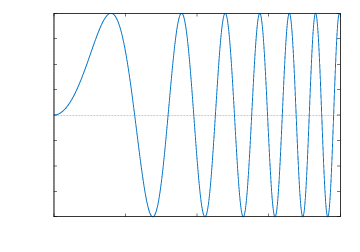
\includegraphics{sinx2}}%
    \gplfronttext
  \end{picture}%
\endgroup
\vspace{-6mm}
 \end{center}
 \caption[]{\quad $y=2\,\sin\;( x^2 )$}
 \label{fig:exmp2sinx2}
\end{figure}

 Notice how the curve ``speeds up'' as $x$ gets larger, making the ``waves'' narrower and narrower.
 Thus, $y=2\,\sin\;( x^2 )$ has no period. Despite this, it appears that the function does have an
 amplitude, namely $2$. To see why, note that since $\abs{\sin\;\theta} \le 1$ for all $\theta$, we
 have
 \begin{displaymath}
  \abs{2\,\sin\;( x^2 )} ~=~ \abs{2} \;\cdot\; \abs{\sin\;( x^2 )} ~\le~ 2 \;\cdot\; 1 ~=~ 2 ~.
 \end{displaymath}
 In the exercises you will be asked to find values of $x$ such that $2\,\sin\;( x^2 )$ reaches the
 maximum value $2$ and the minimum value $-2$. Thus, the amplitude is indeed $2$.\\Note: This curve
 is still sinusoidal despite not being periodic, since the general shape is still that of a ``sine
 wave'', albeit one with variable \emph{cycles}.
\end{exmp}\vspace{-3mm}
\divider
\vspace{1mm}

So far in our examples we have been able to determine the amplitudes of sinusoidal curves fairly
easily. This will not always be the case.
\newpage
\begin{exmp}\label{exmp:3sinx4cosx}
  Find the amplitude and period of $y=3\,\sin\;x + 4\,\cos\;x$.\vspace{1mm}
 \par\noindent\textbf{Solution:} This is sometimes called a \emph{combination} sinusoidal curve, since
 it is the sum of two such curves. The period is still simple to determine: since
 $\sin\;x$ and $\cos\;x$ each repeat every $2\pi$ radians, then so does the combination
 $3\,\sin\;x + 4\,\cos\;x$. Thus, $y=3\,\sin\;x + 4\,\cos\;x$ has period $2\pi$. We can see this in
 the graph, shown in Figure \ref{fig:exmp3sinx4cosx}:\vspace{-1mm}

\begin{figure}[h]
 \begin{center}
   % GNUPLOT: LaTeX picture with Postscript
\begingroup
\footnotesize
  \makeatletter
  \providecommand\color[2][]{%
    \GenericError{(gnuplot) \space\space\space\@spaces}{%
      Package color not loaded in conjunction with
      terminal option `colourtext'%
    }{See the gnuplot documentation for explanation.%
    }{Either use 'blacktext' in gnuplot or load the package
      color.sty in LaTeX.}%
    \renewcommand\color[2][]{}%
  }%
  \providecommand\includegraphics[2][]{%
    \GenericError{(gnuplot) \space\space\space\@spaces}{%
      Package graphicx or graphics not loaded%
    }{See the gnuplot documentation for explanation.%
    }{The gnuplot epslatex terminal needs graphicx.sty or graphics.sty.}%
    \renewcommand\includegraphics[2][]{}%
  }%
  \providecommand\rotatebox[2]{#2}%
  \@ifundefined{ifGPcolor}{%
    \newif\ifGPcolor
    \GPcolortrue
  }{}%
  \@ifundefined{ifGPblacktext}{%
    \newif\ifGPblacktext
    \GPblacktexttrue
  }{}%
  % define a \g@addto@macro without @ in the name:
  \let\gplgaddtomacro\g@addto@macro
  % define empty templates for all commands taking text:
  \gdef\gplbacktext{}%
  \gdef\gplfronttext{}%
  \makeatother
  \ifGPblacktext
    % no textcolor at all
    \def\colorrgb#1{}%
    \def\colorgray#1{}%
  \else
    % gray or color?
    \ifGPcolor
      \def\colorrgb#1{\color[rgb]{#1}}%
      \def\colorgray#1{\color[gray]{#1}}%
      \expandafter\def\csname LTw\endcsname{\color{white}}%
      \expandafter\def\csname LTb\endcsname{\color{black}}%
      \expandafter\def\csname LTa\endcsname{\color{black}}%
      \expandafter\def\csname LT0\endcsname{\color[rgb]{1,0,0}}%
      \expandafter\def\csname LT1\endcsname{\color[rgb]{0,1,0}}%
      \expandafter\def\csname LT2\endcsname{\color[rgb]{0,0,1}}%
      \expandafter\def\csname LT3\endcsname{\color[rgb]{1,0,1}}%
      \expandafter\def\csname LT4\endcsname{\color[rgb]{0,1,1}}%
      \expandafter\def\csname LT5\endcsname{\color[rgb]{1,1,0}}%
      \expandafter\def\csname LT6\endcsname{\color[rgb]{0,0,0}}%
      \expandafter\def\csname LT7\endcsname{\color[rgb]{1,0.3,0}}%
      \expandafter\def\csname LT8\endcsname{\color[rgb]{0.5,0.5,0.5}}%
    \else
      % gray
      \def\colorrgb#1{\color{black}}%
      \def\colorgray#1{\color[gray]{#1}}%
      \expandafter\def\csname LTw\endcsname{\color{white}}%
      \expandafter\def\csname LTb\endcsname{\color{black}}%
      \expandafter\def\csname LTa\endcsname{\color{black}}%
      \expandafter\def\csname LT0\endcsname{\color{black}}%
      \expandafter\def\csname LT1\endcsname{\color{black}}%
      \expandafter\def\csname LT2\endcsname{\color{black}}%
      \expandafter\def\csname LT3\endcsname{\color{black}}%
      \expandafter\def\csname LT4\endcsname{\color{black}}%
      \expandafter\def\csname LT5\endcsname{\color{black}}%
      \expandafter\def\csname LT6\endcsname{\color{black}}%
      \expandafter\def\csname LT7\endcsname{\color{black}}%
      \expandafter\def\csname LT8\endcsname{\color{black}}%
    \fi
  \fi
  \setlength{\unitlength}{0.0500bp}%
  \begin{picture}(7200.00,5040.00)%
    \gplgaddtomacro\gplbacktext{%
      \csname LTb\endcsname%
      \put(682,704){\makebox(0,0)[r]{\strut{}-5}}%
      \csname LTb\endcsname%
      \put(682,1111){\makebox(0,0)[r]{\strut{}-4}}%
      \csname LTb\endcsname%
      \put(682,1518){\makebox(0,0)[r]{\strut{}-3}}%
      \csname LTb\endcsname%
      \put(682,1925){\makebox(0,0)[r]{\strut{}-2}}%
      \csname LTb\endcsname%
      \put(682,2332){\makebox(0,0)[r]{\strut{}-1}}%
      \csname LTb\endcsname%
      \put(682,2740){\makebox(0,0)[r]{\strut{} 0}}%
      \csname LTb\endcsname%
      \put(682,3147){\makebox(0,0)[r]{\strut{} 1}}%
      \csname LTb\endcsname%
      \put(682,3554){\makebox(0,0)[r]{\strut{} 2}}%
      \csname LTb\endcsname%
      \put(682,3961){\makebox(0,0)[r]{\strut{} 3}}%
      \csname LTb\endcsname%
      \put(682,4368){\makebox(0,0)[r]{\strut{} 4}}%
      \csname LTb\endcsname%
      \put(682,4775){\makebox(0,0)[r]{\strut{} 5}}%
      \csname LTb\endcsname%
      \put(814,484){\makebox(0,0){\strut{}$0$}}%
      \csname LTb\endcsname%
      \put(1563,484){\makebox(0,0){\strut{}$\frac{\pi}{2}$}}%
      \csname LTb\endcsname%
      \put(2311,484){\makebox(0,0){\strut{}$\pi$}}%
      \csname LTb\endcsname%
      \put(3060,484){\makebox(0,0){\strut{}$\frac{3\pi}{2}$}}%
      \csname LTb\endcsname%
      \put(3809,484){\makebox(0,0){\strut{}$2\pi$}}%
      \csname LTb\endcsname%
      \put(4557,484){\makebox(0,0){\strut{}$\frac{5\pi}{2}$}}%
      \csname LTb\endcsname%
      \put(5306,484){\makebox(0,0){\strut{}$3\pi$}}%
      \csname LTb\endcsname%
      \put(6054,484){\makebox(0,0){\strut{}$\frac{7\pi}{2}$}}%
      \csname LTb\endcsname%
      \put(6803,484){\makebox(0,0){\strut{}$4\pi$}}%
      \csname LTb\endcsname%
      \put(176,2739){\rotatebox{-270}{\makebox(0,0){\strut{}$y$}}}%
      \put(3808,154){\makebox(0,0){\strut{}$x$}}%
    }%
    \gplgaddtomacro\gplfronttext{%
    }%
    \gplbacktext
    \put(0,0){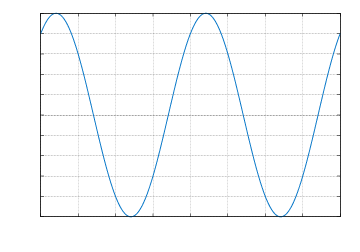
\includegraphics{3sinx4cosx}}%
    \gplfronttext
  \end{picture}%
\endgroup
\vspace{-6mm}
 \end{center}
 \caption[]{\quad $y=3\,\sin\;x + 4\,\cos\;x$}
 \label{fig:exmp3sinx4cosx}
\end{figure}

The graph suggests that the amplitude is $5$, which may not be immediately obvious just by looking at
how the function is defined. In fact, the definition $y=3\,\sin\;x + 4\,\cos\;x$ may tempt you to
think that the amplitude is $7$, since the largest that $3\,\sin\;x$ could be is $3$ and the largest
that $4\,\cos\;x$ could be is $4$, so that the largest their sum could be is $3+4=7$. However,
$3\,\sin\;x$ can never equal $3$ for the same $x$ that makes $4\,\cos\;x$ equal to $4$ (why?).

\piccaption[]{\label{fig:tri345}}\parpic[r]{\begin{tikzpicture}[scale=0.5,
 every node/.style={font=\small}]
 \fill [fill=fillcolor] (0,0) -- (3,0) -- (3,4) -- (0,0);
 \draw (0:1.5) arc (0:53.13:1.5);
 \draw [line width=0.5pt] (2.625,0) -- (2.625,0.375) -- (3,0.375);
 \draw [linecolor,line width=1.5pt] (0,0) -- (3,0) -- (3,4) -- cycle;
 \node [below] at (1.5,0) {$3$};
 \node [right] at (3,2) {$4$};
 \node [above left] at (1.5,2) {$5$};
 \node at (0.9,0.4) {$\theta$};
\end{tikzpicture}}
\picskip{4}
There is a useful technique (which we will discuss further in Chapter 6) for showing that the
amplitude of $y=3\,\sin\;x + 4\,\cos\;x$ is $5$. Let $\theta$ be the angle shown in the right
triangle in Figure \ref{fig:tri345}. Then $\cos\;\theta = \frac{3}{5}$ and $\sin\;\theta =
\frac{4}{5}$. We can use this as follows:
\begin{align*}
 y ~&=~ 3\,\sin\;x ~+~ 4\,\cos\;x\\
 &=~ 5\,\left( \tfrac{3}{5}\,\sin\;x ~+~ \tfrac{4}{5}\,\cos\;x \right)\\
 &=~ 5\,( \cos\;\theta\;\sin\;x ~+~ \sin\;\theta\;\cos\;x )\\
 &=~ 5\,\sin\;(x+\theta)\quad\text{(by the sine addition formula)}
\end{align*}
Thus, $\abs{y} = \abs{5\,\sin\;(x+\theta)} = \abs{5}\,\cdot\,\abs{\sin\;(x+\theta)} \le (5)(1) = 5$,
so the amplitude of $y=3\,\sin\;x + 4\,\cos\;x$ is $5$.
\end{exmp}\vspace{-3mm}
\divider\vspace{-2mm}
\newpage
In general, a combination of sines and cosines will have a period equal to the \emph{lowest common
multiple} of the periods of the sines and cosines being added. In Example \ref{exmp:3sinx4cosx},
$\sin\;x$ and $\cos\;x$ each have period $2\pi$, so the lowest common multiple (which is always an
\emph{integer} multiple) is $1 \,\cdot\, 2\pi = 2\pi$.

\begin{exmp}\label{exmp:cos6xsin4x}
 Find the period of $y=\cos\;6x + \sin\;4x$.\vspace{1mm}
 \par\noindent\textbf{Solution:} The period of $\cos\;6x$ is $\frac{2\pi}{6} = \frac{\pi}{3}$, and the
 period of $\sin\;4x$ is $\frac{2\pi}{4} = \frac{\pi}{2}$. The lowest common multiple of
 $\frac{\pi}{3}$ and $\frac{\pi}{2}$ is $\pi$:
 \begin{alignat*}{4}
  1 \;\cdot\; \tfrac{\pi}{3} ~&=~ \tfrac{\pi}{3} \quad\quad\quad
   &1 \;&\cdot\; \tfrac{\pi}{2} ~&=~ \tfrac{\pi}{2}\\
  2 \;\cdot\; \tfrac{\pi}{3} ~&=~ \tfrac{2\pi}{3} \quad\quad\quad
   &2 \;&\cdot\; \tfrac{\pi}{2} ~&=~ \pi\\
  3 \;\cdot\; \tfrac{\pi}{3} ~&=~ \pi \quad\quad\quad &{} &{}\\
 \end{alignat*}
 Thus, the period of $y=\cos\;6x + \sin\;4x$ is $\pi$. We can see this from its graph in Figure
 \ref{fig:exmpcos6xsin4x}:
 
\begin{figure}[h]
 \begin{center}
   % GNUPLOT: LaTeX picture with Postscript
\begingroup
\footnotesize
  \makeatletter
  \providecommand\color[2][]{%
    \GenericError{(gnuplot) \space\space\space\@spaces}{%
      Package color not loaded in conjunction with
      terminal option `colourtext'%
    }{See the gnuplot documentation for explanation.%
    }{Either use 'blacktext' in gnuplot or load the package
      color.sty in LaTeX.}%
    \renewcommand\color[2][]{}%
  }%
  \providecommand\includegraphics[2][]{%
    \GenericError{(gnuplot) \space\space\space\@spaces}{%
      Package graphicx or graphics not loaded%
    }{See the gnuplot documentation for explanation.%
    }{The gnuplot epslatex terminal needs graphicx.sty or graphics.sty.}%
    \renewcommand\includegraphics[2][]{}%
  }%
  \providecommand\rotatebox[2]{#2}%
  \@ifundefined{ifGPcolor}{%
    \newif\ifGPcolor
    \GPcolortrue
  }{}%
  \@ifundefined{ifGPblacktext}{%
    \newif\ifGPblacktext
    \GPblacktexttrue
  }{}%
  % define a \g@addto@macro without @ in the name:
  \let\gplgaddtomacro\g@addto@macro
  % define empty templates for all commands taking text:
  \gdef\gplbacktext{}%
  \gdef\gplfronttext{}%
  \makeatother
  \ifGPblacktext
    % no textcolor at all
    \def\colorrgb#1{}%
    \def\colorgray#1{}%
  \else
    % gray or color?
    \ifGPcolor
      \def\colorrgb#1{\color[rgb]{#1}}%
      \def\colorgray#1{\color[gray]{#1}}%
      \expandafter\def\csname LTw\endcsname{\color{white}}%
      \expandafter\def\csname LTb\endcsname{\color{black}}%
      \expandafter\def\csname LTa\endcsname{\color{black}}%
      \expandafter\def\csname LT0\endcsname{\color[rgb]{1,0,0}}%
      \expandafter\def\csname LT1\endcsname{\color[rgb]{0,1,0}}%
      \expandafter\def\csname LT2\endcsname{\color[rgb]{0,0,1}}%
      \expandafter\def\csname LT3\endcsname{\color[rgb]{1,0,1}}%
      \expandafter\def\csname LT4\endcsname{\color[rgb]{0,1,1}}%
      \expandafter\def\csname LT5\endcsname{\color[rgb]{1,1,0}}%
      \expandafter\def\csname LT6\endcsname{\color[rgb]{0,0,0}}%
      \expandafter\def\csname LT7\endcsname{\color[rgb]{1,0.3,0}}%
      \expandafter\def\csname LT8\endcsname{\color[rgb]{0.5,0.5,0.5}}%
    \else
      % gray
      \def\colorrgb#1{\color{black}}%
      \def\colorgray#1{\color[gray]{#1}}%
      \expandafter\def\csname LTw\endcsname{\color{white}}%
      \expandafter\def\csname LTb\endcsname{\color{black}}%
      \expandafter\def\csname LTa\endcsname{\color{black}}%
      \expandafter\def\csname LT0\endcsname{\color{black}}%
      \expandafter\def\csname LT1\endcsname{\color{black}}%
      \expandafter\def\csname LT2\endcsname{\color{black}}%
      \expandafter\def\csname LT3\endcsname{\color{black}}%
      \expandafter\def\csname LT4\endcsname{\color{black}}%
      \expandafter\def\csname LT5\endcsname{\color{black}}%
      \expandafter\def\csname LT6\endcsname{\color{black}}%
      \expandafter\def\csname LT7\endcsname{\color{black}}%
      \expandafter\def\csname LT8\endcsname{\color{black}}%
    \fi
  \fi
  \setlength{\unitlength}{0.0500bp}%
  \begin{picture}(7200.00,5040.00)%
    \gplgaddtomacro\gplbacktext{%
      \csname LTb\endcsname%
      \put(946,704){\makebox(0,0)[r]{\strut{}-2}}%
      \csname LTb\endcsname%
      \put(946,1213){\makebox(0,0)[r]{\strut{}-1.5}}%
      \csname LTb\endcsname%
      \put(946,1722){\makebox(0,0)[r]{\strut{}-1}}%
      \csname LTb\endcsname%
      \put(946,2231){\makebox(0,0)[r]{\strut{}-0.5}}%
      \csname LTb\endcsname%
      \put(946,2740){\makebox(0,0)[r]{\strut{} 0}}%
      \csname LTb\endcsname%
      \put(946,3248){\makebox(0,0)[r]{\strut{} 0.5}}%
      \csname LTb\endcsname%
      \put(946,3757){\makebox(0,0)[r]{\strut{} 1}}%
      \csname LTb\endcsname%
      \put(946,4266){\makebox(0,0)[r]{\strut{} 1.5}}%
      \csname LTb\endcsname%
      \put(946,4775){\makebox(0,0)[r]{\strut{} 2}}%
      \csname LTb\endcsname%
      \put(1078,484){\makebox(0,0){\strut{}$0$}}%
      \csname LTb\endcsname%
      \put(2509,484){\makebox(0,0){\strut{}$\frac{\pi}{2}$}}%
      \csname LTb\endcsname%
      \put(3941,484){\makebox(0,0){\strut{}$\pi$}}%
      \csname LTb\endcsname%
      \put(5372,484){\makebox(0,0){\strut{}$\frac{3\pi}{2}$}}%
      \csname LTb\endcsname%
      \put(6803,484){\makebox(0,0){\strut{}$2\pi$}}%
      \put(176,2739){\rotatebox{-270}{\makebox(0,0){\strut{}$y$}}}%
      \put(3940,154){\makebox(0,0){\strut{}$x$}}%
    }%
    \gplgaddtomacro\gplfronttext{%
    }%
    \gplbacktext
    \put(0,0){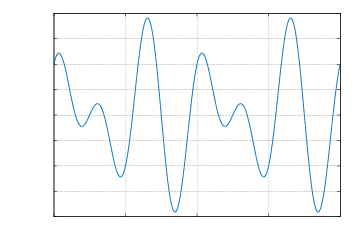
\includegraphics{cos6xsin4x}}%
    \gplfronttext
  \end{picture}%
\endgroup
\vspace{-6mm}
 \end{center}
 \caption[]{\quad $y=\cos\;6x + \sin\;4x$}
 \label{fig:exmpcos6xsin4x}
\end{figure}

 What about the amplitude? Unfortunately we can not use the technique from Example
 \ref{exmp:3sinx4cosx}, since we are not taking the cosine and sine of the same angle; we are
 taking the cosine of $6x$ but the sine of $4x$. In this case, it appears from the graph that the
 maximum is close to $2$ and the minimum is close to $-2$. In Chapter 6, we will describe how to
 use a numerical computation program to show that the maximum and minimum are
 $\pm\,1.90596111871578$, respectively (accurate to within $\approx 2.2204 \times 10^{-16}$). Hence,
 the amplitude is $1.90596111871578$.
\end{exmp}\vspace{-3mm}
\divider\vspace{-2mm}
\newpage
Generalizing Example \ref{exmp:3sinx4cosx}, an expression of the form
$a\,\sin\;\omega x \;+\; b\,\cos\;\omega x$ is equivalent to
$\sqrt{a^2 + b^2}\;\sin\;(x+\theta)$, where $\theta$ is an angle such that
$\cos\;\theta = \frac{a}{\sqrt{a^2 + b^2}}$ and $\sin\;\theta = \frac{b}{\sqrt{a^2 + b^2}}$. So
$y=a\,\sin\;\omega x \;+\; b\,\cos\;\omega x$ will have amplitude $\sqrt{a^2 + b^2}$. Note that this
method only works when the angle $\omega x$ is the same in both the sine and cosine terms.

We have seen how adding a constant to a function shifts the entire graph vertically. We will now see
how to shift the entire graph of a periodic curve horizontally.

\piccaption[]{\enskip $y=A\,\sin\;\omega x$\label{fig:phasenone}}\parpic[r]{\begin{tikzpicture}[scale=1.2,
 every node/.style={font=\small}]
 \begin{scope}[shift={(0,0)},color=linecolor,line width=1.5pt,x=3cm/360]
  \draw[black!60,line width=0.3pt,dotted] (0,-1) grid[xstep=90,ystep=1] (360,1);
  \draw[black!60,line width=0.3pt,-latex] (0,0) -- (380,0) node[right] {$x$};
  \draw[black!60,line width=0.3pt,-latex] (0,-1.2) -- (0,1.6) node[above] {$y$};
  \pgfplothandlerlineto
  \pgfplotfunction{\x}{0,5,...,360}{\pgfpointxy{\x}{sin(\x)}}
  \pgfusepath{stroke}
  \node[black,left] at (0,0) {$0$};
  \foreach \pos in {90,180,270,360}
   \draw[black!60,line width=0.3pt,shift={(\pos,0)}] (0pt,3pt) -- (0pt,-3pt);
  \foreach \pos in {-1,1}
   \draw[black!60,line width=0.3pt,shift={(0,\pos)}] (3pt,0pt) -- (-3pt,0pt);
  \node[black,left] at (0,1) {$A$};
  \node[black,left] at (0,-1) {$-A$};
  \node[black,below] at (180,-0.1) {$\tfrac{\pi}{\omega}$};
  \node[black,below] at (360,-0.1) {$\tfrac{2\pi}{\omega}$};
 \end{scope}
 \begin{scope}[>=latex]
  \draw [<->|] (0,1.3) -- (3,1.3) node[midway,fill=white] {period $= \tfrac{2\pi}{\omega}$};
 \end{scope}
\end{tikzpicture}}
Consider a function of the form $y=A\,\sin\;\omega x$, where $A$ and $\omega$ are nonzero constants.
For simplicity we will assume that $A >0$ and $\omega > 0$ (in general either one could be
negative). Then the amplitude is $A$ and the period is $\frac{2\pi}{\omega}$. The graph is shown in
Figure \ref{fig:phasenone}.

Now consider the function $y=A\,\sin\;(\omega x + \phi)$, where $\phi$ is some constant. The
amplitude is still $A$, and the period is still $\frac{2\pi}{\omega}$, since $\omega x + \phi$ is a
linear function of $x$. Also, we know that the sine function goes through an entire cycle when its
angle goes from $0$ to $2\pi$. Here, we are taking the sine of the angle $\omega x + \phi$. So as
$\omega x + \phi$ goes from $0$ to $2\pi$, an entire cycle of the function
$y=A\,\sin\;(\omega x + \phi)$ will be traced out. That cycle starts when
\begin{align*}
 \omega x + \phi ~=~ 0 \quad&\Rightarrow\quad x ~=~ -\frac{\phi}{\omega}\\
\intertext{and ends when}
 \omega x + \phi ~=~ 2\pi \quad&\Rightarrow\quad x ~=~ \frac{2\pi}{\omega}\;-\;\frac{\phi}{\omega}~.
\end{align*}
Thus, the graph of $y=A\,\sin\;(\omega x + \phi)$ is just the graph of $y=A\,\sin\;\omega x$
shifted horizontally by $\frac{-\phi}{\omega}$, as in Figure \ref{fig:phaseshift}. The quantity $\phi$ is the phase. The graph is
shifted to the right when $\phi <0$, and to the left when $\phi >0$. The amount
$-\frac{\phi}{\omega}$ of the shift is called the \textbf{phase shift}\index{phase shift} of the
graph.  The phase has units of radians, whereas the phase shift has the same units as the $x$ axis.

\begin{figure}[h]
 \centering
 \subfloat[][ $\phi <0$: right shift]{
  \begin{tikzpicture}[scale=1.2,every node/.style={font=\small}]
   \begin{scope}[shift={(0,0)},color=linecolor,line width=1.5pt,x=3cm/360]
	\draw[black!60,line width=0.3pt,-latex] (0,0) -- (500,0) node[right] {$x$};
	\draw[black!60,line width=0.3pt,-latex] (0,-1.2) -- (0,1.7) node[above] {$y$};
	\pgfplothandlerlineto
	\pgfplotfunction{\x}{90,95,...,450}{\pgfpointxy{\x}{sin(-90+\x)}}
	\pgfusepath{stroke}
	\node[black,left] at (0,0) {$0$};
	\foreach \pos in {90,180,270,360,450}
	 \draw[black!60,line width=0.3pt,shift={(\pos,0)}] (0pt,3pt) -- (0pt,-3pt);
	\foreach \pos in {-1,1}
	 \draw[black!60,line width=0.3pt,shift={(0,\pos)}] (3pt,0pt) -- (-3pt,0pt);
	\node[black,left] at (0,1) {$A$};
	\node[black,left] at (0,-1) {$-A$};
	\node[black,below right] at (425,-0.1) {$\tfrac{2\pi}{\omega}+\tfrac{\phi}{\omega}$};
	\node[black,below] at (90,-0.1) {$\tfrac{\phi}{\omega}$};
   \end{scope}
   \begin{scope}[>=latex]
    \draw [|<->|] (0.75,1.4) -- (3.75,1.4) node[midway,fill=white]
	 {period $= \tfrac{2\pi}{\omega}$};
    \draw [<->|] (0,-0.9) -- (0.75,-0.9);
	\node[below right] at (0,-0.9) {phase shift};
   \end{scope}
  \end{tikzpicture}}
 \qquad\qquad
 \subfloat[][ $\phi >0$: left shift]{
  \begin{tikzpicture}[scale=1.2,every node/.style={font=\small}]
   \begin{scope}[shift={(0,0)},color=linecolor,line width=1.5pt,x=3cm/360]
	\draw[black!60,line width=0.3pt,-latex] (-120,0) -- (320,0) node[right] {$x$};
	\draw[black!60,line width=0.3pt,-latex] (0,-1.2) -- (0,1.7) node[above] {$y$};
	\pgfplothandlerlineto
	\pgfplotfunction{\x}{-90,-85,...,270}{\pgfpointxy{\x}{sin(90+\x)}}
	\pgfusepath{stroke}
	\node[black,below right] at (0,0) {$0$};
	\foreach \pos in {-90,90,180,270}
	 \draw[black!60,line width=0.3pt,shift={(\pos,0)}] (0pt,3pt) -- (0pt,-3pt);
	\foreach \pos in {-1,1}
	 \draw[black!60,line width=0.3pt,shift={(0,\pos)}] (3pt,0pt) -- (-3pt,0pt);
	\node[black,left] at (0,1.1) {$A$};
	\node[black,right] at (0,-1) {$-A$};
	\node[black,below right] at (245,-0.1) {$\tfrac{2\pi}{\omega}+\tfrac{\phi}{\omega}$};
	\node[black,below] at (-90,-0.1) {$\tfrac{\phi}{\omega}$};
   \end{scope}
   \begin{scope}[>=latex]
    \draw [|<->|] (-0.75,1.4) -- (2.25,1.4) node[pos=0.6,fill=white]
	 {period $= \tfrac{2\pi}{\omega}$};
    \draw [|<->] (-0.75,-0.9) -- (0,-0.9);
	\node[below left] at (0,-0.9) {phase shift};
   \end{scope}
  \end{tikzpicture}}\vspace{-2mm}
 \caption[]{\quad Phase shift for $y=A\,\sin\;(\omega x + \phi)$}
 \label{fig:phaseshift}
\end{figure}
\newpage
The phase shift is defined similarly for the other trigonometric functions.

\begin{exmp}
 Find the amplitude, period, and phase shift of $y=3\,\cos\;(2x - \pi)$.\vspace{1mm}
 \par\noindent\textbf{Solution:} The amplitude is $3$, the period is $\frac{2\pi}{2} = \pi$, and the
 phase shift is $\frac{\pi}{2}$. The graph is shown in Figure \ref{fig:exmp3cos2mpi}:\vspace{-1mm}

\begin{figure}[h]
 \begin{center}
  \begin{tikzpicture}[scale=1.2,every node/.style={font=\small}]
   \begin{scope}[shift={(0,0)},color=linecolor,line width=1.5pt,x=8cm/360,y=1.5cm/3]
    \draw[black!60,line width=0.3pt,dotted] (0,-3) grid[xstep=90,ystep=1] (360,3);
	\draw[black!60,line width=0.3pt,-latex] (0,0) -- (380,0) node[right] {$x$};
	\draw[black!60,line width=0.3pt,-latex] (0,-3.8) -- (0,3.8) node[above] {$y$};
	\pgfplothandlerlineto
	\pgfplotfunction{\x}{0,5,...,360}{\pgfpointxy{\x}{3*cos(-180+2*\x)}}
	\pgfusepath{stroke}
	\node[black,left] at (0,0) {$0$};
	\foreach \pos in {90,180,270,360}
	 \draw[black!60,line width=0.3pt,shift={(\pos,0)}] (0pt,3pt) -- (0pt,-3pt);
	\foreach \pos in {-3,-2,-1,1,2,3}
	 \draw[black!60,line width=0.3pt,shift={(0,\pos)}] (3pt,0pt) -- (-3pt,0pt) node[black,left]
	  {$\pos$};
	\node[black,below] at (90,-0.1) {$\tfrac{\pi}{2}$};
	\node[black,below] at (180,-0.1) {$\pi$};
	\node[black,below] at (270,-0.1) {$\tfrac{3\pi}{2}$};
	\node[black,below] at (360,-0.1) {$2\pi$};
   \end{scope}
   \begin{scope}[>=latex]
    \draw [|<->|] (2,1.9) -- (6,1.9) node[midway,fill=white] {period $= \pi$};
    \draw [<->|] (0,-1.7) -- (2,-1.7);
	\node[below right] at (0,-1.7) {phase shift $= \tfrac{\pi}{2}$};
    \draw [|<->|] (-0.9,0) -- (-0.9,1.5) node[midway,left] {amplitude $= 3$};
   \end{scope}
  \end{tikzpicture}\vspace{-6mm}
 \end{center}
 \caption[]{\quad $y=3\,\cos\;(2x - \pi)$}
 \label{fig:exmp3cos2mpi}
\end{figure}

Notice that the graph is the same as the graph of $y=3\,\cos\;2x$ shifted to the right by
$\frac{\pi}{2}$, the amount of the phase shift.
\end{exmp}
\begin{exmp}
 Find the amplitude, period, and phase shift of $y=-2\,\sin\;\left(3x +
 \frac{\pi}{2}\right)$.\vspace{1mm}
 \par\noindent\textbf{Solution:} The amplitude is $2$, the period is $\frac{2\pi}{3}$, and the
 phase shift is $\frac{-\frac{\pi}{2}}{3} = -\frac{\pi}{6}$. Notice the negative sign in the phase
 shift, since $3x+\pi=3x-(-\pi)$ is in the form $\omega x - \phi$. The graph is shown in Figure
 \ref{fig:exmpm2sin3ppi2}:\vspace{-1mm}

\begin{figure}[h]
 \begin{center}
  \begin{tikzpicture}[scale=1.1,every node/.style={font=\small}]
   \begin{scope}[shift={(0,0)},color=linecolor,line width=1.5pt,x=8cm/240,y=1.5cm/2]
    \draw[black!60,line width=0.3pt,dotted] (-30,-2) grid[xstep=30,ystep=1] (240,2);
	\draw[black!60,line width=0.3pt,-latex] (-50,0) -- (250,0) node[right] {$x$};
	\draw[black!60,line width=0.3pt,-latex] (0,-2.8) -- (0,2.8) node[above] {$y$};
	\pgfplothandlerlineto
	\pgfplotfunction{\x}{-30,-25,...,240}{\pgfpointxy{\x}{-2*sin(90+3*\x)}}
	\pgfusepath{stroke}
	\node[black,below left] at (0,0) {$0$};
	\foreach \pos in {-30,30,60,90,120,150,180,210,240}
	 \draw[black!60,line width=0.3pt,shift={(\pos,0)}] (0pt,3pt) -- (0pt,-3pt);
	\foreach \pos in {-2,-1,1,2}
	 \draw[black!60,line width=0.3pt,shift={(0,\pos)}] (3pt,0pt) -- (-3pt,0pt) node[black,left]
	  {$\pos$};
	\node[black,below] at (-35,-0.1) {$-\tfrac{\pi}{6}$};
	\node[black,below] at (30,-0.1) {$\tfrac{\pi}{6}$};
	\node[black,below] at (60,-0.1) {$\tfrac{\pi}{3}$};
	\node[black,below] at (90,-0.1) {$\tfrac{\pi}{2}$};
	\node[black,below] at (120,-0.1) {$\tfrac{2\pi}{3}$};
	\node[black,below] at (150,-0.1) {$\tfrac{5\pi}{6}$};
	\node[black,below] at (180,-0.1) {$\pi$};
	\node[black,below] at (210,-0.1) {$\tfrac{7\pi}{6}$};
	\node[black,below] at (240,-0.1) {$\tfrac{4\pi}{3}$};
   \end{scope}
   \begin{scope}[>=latex]
    \draw [|<->|] (-1,1.9) -- (3,1.9) node[pos=0.55,fill=white] {period $= \frac{2\pi}{3}$};
    \draw [|<->] (-1,-1.7) -- (0,-1.7);
	\node[below left] at (0,-1.75) {phase shift $= -\tfrac{\pi}{6}$};
    \draw [|<->|] (-1.1,0) -- (-1.1,1.5) node[midway,left] {amplitude $= 2$};
   \end{scope}
  \end{tikzpicture}\vspace{-6mm}
 \end{center}
 \caption[]{\quad $y=-2\,\sin\;\left( 3x + \frac{\pi}{2} \right)$}
 \label{fig:exmpm2sin3ppi2}
\end{figure}
\end{exmp}\vspace{-4mm}
\divider\vspace{-2mm}
\newpage
In engineering two periodic functions with the same period are said to be \emph{out of
phase} if their phase shifts differ. For example, $\sin\;\left( x -
\frac{\pi}{6} \right)$ and $\sin\;x$ would be $\frac{\pi}{6}$ radians (or $30\Degrees$) out of
phase, and $\sin\;x$ would be said to \emph{lag} $\sin\;\left( x - \frac{\pi}{6} \right)$ by
$\frac{\pi}{6}$ radians, while $\sin\;\left( x - \frac{\pi}{6} \right)$ \emph{leads}
$\sin\;x$ by $\frac{\pi}{6}$ radians. Periodic functions with the same period and the same phase
shift are \emph{in phase}.\index{phase, out of or in}

The following is a summary of the properties of trigonometric graphs:

\begin{center}\statecomment{For any constants $A \ne 0$, $\omega \ne 0$, and $\phi$:
\begin{align*}
 y = A\,\sin\;(\omega x + \phi) ~~&\text{has amplitude $\abs{A}$, period $\tfrac{2\pi}{\omega}$, and
  phase shift $\tfrac{-\phi}{\omega}$}\\
 y = A\,\cos\;(\omega x + \phi) ~~&\text{has amplitude $\abs{A}$, period $\tfrac{2\pi}{\omega}$, and
  phase shift $\tfrac{-\phi}{\omega}$}\\
 y = A\,\tan\;(\omega x + \phi) ~~&\text{has undefined amplitude, period $\tfrac{\pi}{\omega}$, and
  phase shift $\tfrac{-\phi}{\omega}$}\\
 y = A\,\csc\;(\omega x + \phi) ~~&\text{has undefined amplitude, period $\tfrac{2\pi}{\omega}$, and
  phase shift $\tfrac{-\phi}{\omega}$}\\
 y = A\,\sec\;(\omega x + \phi) ~~&\text{has undefined amplitude, period $\tfrac{2\pi}{\omega}$, and
  phase shift $\tfrac{-\phi}{\omega}$}\\
 y = A\,\cot\;(\omega x + \phi) ~~&\text{has undefined amplitude, period $\tfrac{\pi}{\omega}$, and
  phase shift $\tfrac{-\phi}{\omega}$}
\end{align*}}\end{center}\vspace{-4mm}

\divider
\vspace{2mm}

\startexercises\label{sec5dot2}
\vspace{5mm}
{\small
\par\noindent For Exercises 1-12, find the amplitude, period, and phase shift of the given function.
Then graph one cycle of the function, either by hand or by using Gnuplot (see Appendix B).
\begin{enumerate}[\bfseries 1.]
\begin{multicols}{4}
 \item $y=3\,\cos\;\pi x$
 \item $y=\sin\;(2\pi x - \pi)$
 \item $y=-\sin\;(5x + 3)$
 \item $y=1+8\,\cos\;(6x- \pi)$
\end{multicols}
\begin{multicols}{4}
 \item $y=2+\cos\;(5x + \pi)$
 \item $y=1-\sin\;(3\pi - 2x)$
 \item $y=1-\cos\;(3\pi - 2x)$
 \item $y=2\,\tan\;(x - 1)$
\end{multicols}
\begin{multicols}{4}
 \item $y=1-\tan\;(3\pi - 2x)$
 \item $y=\sec\;(2x + 1)$
 \item $y=2\csc\;(2x - 1)$
 \item $y=2+4\,\cot\;(1-x)$
\end{multicols}
 \item For the function $y=2\,\sin\;( x^2 )$ in Example \ref{exmp:2sinx2}, for which values of $x$
  does the function reach its maximum value $2$, and for which values of $x$ does it reach
  its minimum value $-2\,$?
 \item For the function $y=3\,\sin\;x + 4\,\cos\;x$ in Example \ref{exmp:3sinx4cosx}, for which
  values of $x$ does the function reach its maximum value $5$, and for which values of $x$ does it
  reach its minimum value $-5\,$? You can restrict your answers to be between $0$ and $2\pi$.
 \item Graph the function $y=\sin^2 \,x$ from $x=0$ to $x=2\pi$, either by hand or by using Gnuplot.
  What are the amplitude and period of this function?
 \item\label{exer:circuitphase}
  The current $i(t)$ in an AC electrical circuit at time $t\ge 0$ is given by
  $i(t) = I_m \,\sin\;\omega t$, and the voltage $v(t)$ is given by $v(t) = V_m \,\sin\;\omega t$,
  where $V_m > I_m > 0$ and $\omega > 0$ are constants.
  Sketch one cycle of both $i(t)$ and $v(t)$ \emph{together on the same graph} (i.e. on the same set
  of axes). Are the current and voltage in phase or out of phase?
 \item Repeat Exercise \ref{exer:circuitphase} with $i(t)$ the same as before but with $v(t)=
  V_m \,\sin\;\left(\omega t + \frac{\pi}{4}\right)$.
 \item Repeat Exercise \ref{exer:circuitphase} with
  $i(t)=-I_m \,\cos\;\left(\omega t - \frac{\pi}{3}\right)$ and $v(t)=
  V_m \,\sin\;\left(\omega t - \frac{5\pi}{6}\right)$.
\suspend{enumerate}
 For Exercises \ref{exer:ampcombostart}-\ref{exer:ampcomboend}, find the amplitude and period of
 the given function. Then graph one cycle of the function, either by hand or by using Gnuplot.
\resume{enumerate}[{[\bfseries 1.]}]
\begin{multicols}{3}
 \item\label{exer:ampcombostart} $y=3\,\sin\;\pi x \;-\; 5\,\cos\;\pi x$
 \item $y=-5\,\sin\;3x \;+\; 12\,\cos\;3x$
 \item\label{exer:ampcomboend} $y=2\,\cos\;x \;+\; 2\,\sin\;x$
\end{multicols}
 \item Find the amplitude of the function $y=2\,\sin\;( x^2 ) \;+\; \cos\;( x^2 )$.
\suspend{enumerate}
 For Exercises \ref{exer:percombostart}-\ref{exer:percomboend}, find the period of the given
 function. Graph one cycle using Gnuplot.
\resume{enumerate}[{[\bfseries 1.]}]
\begin{multicols}{3}
 \item\label{exer:percombostart} $y=\sin\;3x \;-\; \cos\;5x$
 \item $y=\sin\;\frac{x}{3} \;+\; 2\,\cos\;\frac{3x}{4}$
 \item\label{exer:percomboend} $y=2\,\sin\;\pi x \;+\; 3\,\cos\;\frac{\pi}{3}x$
\end{multicols}
 \item Let $y = 0.5\,\sin\;x ~\sin\;12x\,$. Its graph for $x$ from $0$ to $4\pi$ is shown in
  Figure \ref{fig:modulated}:

\begin{figure}[h]
 \begin{center}
   % GNUPLOT: LaTeX picture with Postscript
\begingroup
\footnotesize
  \makeatletter
  \providecommand\color[2][]{%
    \GenericError{(gnuplot) \space\space\space\@spaces}{%
      Package color not loaded in conjunction with
      terminal option `colourtext'%
    }{See the gnuplot documentation for explanation.%
    }{Either use 'blacktext' in gnuplot or load the package
      color.sty in LaTeX.}%
    \renewcommand\color[2][]{}%
  }%
  \providecommand\includegraphics[2][]{%
    \GenericError{(gnuplot) \space\space\space\@spaces}{%
      Package graphicx or graphics not loaded%
    }{See the gnuplot documentation for explanation.%
    }{The gnuplot epslatex terminal needs graphicx.sty or graphics.sty.}%
    \renewcommand\includegraphics[2][]{}%
  }%
  \providecommand\rotatebox[2]{#2}%
  \@ifundefined{ifGPcolor}{%
    \newif\ifGPcolor
    \GPcolortrue
  }{}%
  \@ifundefined{ifGPblacktext}{%
    \newif\ifGPblacktext
    \GPblacktexttrue
  }{}%
  % define a \g@addto@macro without @ in the name:
  \let\gplgaddtomacro\g@addto@macro
  % define empty templates for all commands taking text:
  \gdef\gplbacktext{}%
  \gdef\gplfronttext{}%
  \makeatother
  \ifGPblacktext
    % no textcolor at all
    \def\colorrgb#1{}%
    \def\colorgray#1{}%
  \else
    % gray or color?
    \ifGPcolor
      \def\colorrgb#1{\color[rgb]{#1}}%
      \def\colorgray#1{\color[gray]{#1}}%
      \expandafter\def\csname LTw\endcsname{\color{white}}%
      \expandafter\def\csname LTb\endcsname{\color{black}}%
      \expandafter\def\csname LTa\endcsname{\color{black}}%
      \expandafter\def\csname LT0\endcsname{\color[rgb]{1,0,0}}%
      \expandafter\def\csname LT1\endcsname{\color[rgb]{0,1,0}}%
      \expandafter\def\csname LT2\endcsname{\color[rgb]{0,0,1}}%
      \expandafter\def\csname LT3\endcsname{\color[rgb]{1,0,1}}%
      \expandafter\def\csname LT4\endcsname{\color[rgb]{0,1,1}}%
      \expandafter\def\csname LT5\endcsname{\color[rgb]{1,1,0}}%
      \expandafter\def\csname LT6\endcsname{\color[rgb]{0,0,0}}%
      \expandafter\def\csname LT7\endcsname{\color[rgb]{1,0.3,0}}%
      \expandafter\def\csname LT8\endcsname{\color[rgb]{0.5,0.5,0.5}}%
    \else
      % gray
      \def\colorrgb#1{\color{black}}%
      \def\colorgray#1{\color[gray]{#1}}%
      \expandafter\def\csname LTw\endcsname{\color{white}}%
      \expandafter\def\csname LTb\endcsname{\color{black}}%
      \expandafter\def\csname LTa\endcsname{\color{black}}%
      \expandafter\def\csname LT0\endcsname{\color{black}}%
      \expandafter\def\csname LT1\endcsname{\color{black}}%
      \expandafter\def\csname LT2\endcsname{\color{black}}%
      \expandafter\def\csname LT3\endcsname{\color{black}}%
      \expandafter\def\csname LT4\endcsname{\color{black}}%
      \expandafter\def\csname LT5\endcsname{\color{black}}%
      \expandafter\def\csname LT6\endcsname{\color{black}}%
      \expandafter\def\csname LT7\endcsname{\color{black}}%
      \expandafter\def\csname LT8\endcsname{\color{black}}%
    \fi
  \fi
  \setlength{\unitlength}{0.0500bp}%
  \begin{picture}(7200.00,5040.00)%
    \gplgaddtomacro\gplbacktext{%
      \csname LTb\endcsname%
      \put(946,704){\makebox(0,0)[r]{\strut{}-1}}%
      \put(946,1722){\makebox(0,0)[r]{\strut{}-0.5}}%
      \put(946,2740){\makebox(0,0)[r]{\strut{} 0}}%
      \put(946,3757){\makebox(0,0)[r]{\strut{} 0.5}}%
      \put(946,4775){\makebox(0,0)[r]{\strut{} 1}}%
      \put(1078,484){\makebox(0,0){\strut{}$0$}}%
      \put(2509,484){\makebox(0,0){\strut{}$\pi$}}%
      \put(3941,484){\makebox(0,0){\strut{}$2\pi$}}%
      \put(5372,484){\makebox(0,0){\strut{}$3\pi$}}%
      \put(6803,484){\makebox(0,0){\strut{}$4\pi$}}%
      \csname LTb\endcsname%
      \put(176,2739){\rotatebox{-270}{\makebox(0,0){\strut{}$y$}}}%
      \put(3940,154){\makebox(0,0){\strut{}$x$}}%
    }%
    \gplgaddtomacro\gplfronttext{%
      \csname LTb\endcsname%
      \put(5816,4602){\makebox(0,0)[r]{\strut{}$0.5*\sin(x)*\sin(12*x)$}}%
      \csname LTb\endcsname%
      \put(5816,4382){\makebox(0,0)[r]{\strut{}$0.5*\sin(x)$}}%
      \csname LTb\endcsname%
      \put(5816,4162){\makebox(0,0)[r]{\strut{}$-0.5*\sin(x)$}}%
    }%
    \gplbacktext
    \put(0,0){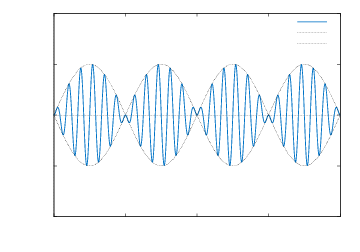
\includegraphics{modulated}}%
    \gplfronttext
  \end{picture}%
\endgroup
\vspace{-6mm}
 \end{center}
 \caption[]{\quad Modulated wave $y=0.5\,\sin\;x ~\sin\;12x$}
 \label{fig:modulated}
\end{figure}

  You can think of this function as $\sin\;12x$ with a sinusoidally varying ``amplitude''of
  $0.5\,\sin\;x$. What is the period of this function?
  From the graph it looks like the amplitude may be $0.5$.
  Without finding the exact amplitude, explain why the amplitude is in fact \emph{less} than $0.5$.
  The function above is known as a \emph{modulated wave}\index{modulated wave}, and the functions
  $\pm\,0.5\,\sin\;x$ form an \emph{amplitude envelope}\index{amplitude envelope} for the wave (i.e.
  they enclose the wave). Use an identity from Section 3.4 to write this function as a sum of
  sinusoidal curves.
 \item Use Gnuplot to graph the function $y= x^2 \,\sin\;10x$ from $x = -2\pi$ to $x=2\pi$. What
  functions form its amplitude envelope? (Note: Use \texttt{set samples 500} in Gnuplot.)
 \item Use Gnuplot to graph the function $y= \frac{1}{x^2} \,\sin\;80x$ from $x = 0.2$ to $x=\pi$.
  What functions form its amplitude envelope? (Note: Use \texttt{set samples 500} in Gnuplot.)
 \item Does the function $y=\sin\;\pi x \;+\; \cos\;x$ have a period? Explain your answer.
 \item Use Gnuplot to graph the function $y=\frac{\sin\;x}{x}$ from $x=-4\pi$ to $x=4\pi$. What
  happens at $x=0$?
\end{enumerate}}



\centerline{\textbf{Properties of the Sinusoid \boldmath  $S(t) = A \sin(\omega t + \phi) + B$}} \index{sinusoid ! properties of}



% % % % % % % % % % % % % % % % % % % % % % % % % % % % % % % % % % % %new section


\newpage
%Begin Section 5.3
\section{Applications of Sinusoids}

\label{Sinusoid}

 The cosine and sine functions can be used to model their fair share of natural behaviors. In the previous section, we introduced the concept of a sinusoid as a function which can be written either in the form $C(x) = A \cos(\omega x + \phi) + B$ for $\omega > 0$ or equivalently, in the form $S(x) = A \sin(\omega x + \phi) + B$ for $\omega > 0$.  At the time, we remained undecided as to which form we preferred, but the time for such indecision is over.  For clarity of exposition we focus on the sine function\footnote{Sine haters can use the co-function identity $\cos\left(\frac{\pi}{2} - \theta\right) = \sin(\theta)$ to turn all of the sines into cosines.} in this section and switch to the independent variable $t$, since the applications in this section are time-dependent.  We reintroduce and summarize all of the important facts and definitions about this form of the sinusoid below.

\smallskip

\colorbox{ResultColor}{\bbm

\phantomsection
\label{sinesinusoidprops}

\centerline{\textbf{Properties of the Sinusoid \boldmath  $S(t) = A \sin(\omega t + \phi) + B$}} \index{sinusoid ! properties of}

\begin{itemize}

\item  The \textbf{amplitude}\index{sinusoid ! amplitude}\index{amplitude} is $|A|$

\item  The \textbf{angular frequency}\index{sinusoid ! frequency ! angular}\index{frequency ! angular} is $\omega$ and the \textbf{ordinary frequency}\index{sinusoid ! frequency ! ordinary}\index{frequency ! ordinary} is $f  = \dfrac{\omega}{2\pi}$

\item  The \textbf{period}\index{sinusoid ! period}\index{period ! of a sinusoid} is  $T = \dfrac{1}{f} = \dfrac{2\pi}{\omega}$

\item  The \textbf{phase}\index{sinusoid ! phase}\index{phase} is $\phi$ and the \textbf{phase shift}\index{sinusoid ! phase shift}\index{phase shift} is $-\dfrac{\phi}{\omega}$

\item  The \textbf{vertical shift}\index{sinusoid ! vertical shift}\index{sinusoid ! baseline} or \textbf{baseline} is $B$

\end{itemize}

\ebm}

\medskip

Along with knowing these formulas, it is helpful to remember what these quantities mean in context.  The amplitude measures the maximum displacement of the sine wave from its baseline (determined by the vertical shift), the period is the length of time it takes to complete one cycle of the sinusoid, the angular frequency tells how many cycles are completed over an interval of length $2\pi$, and the ordinary frequency measures how many cycles occur per unit of time. The phase indicates what angle $\phi$ corresponds to $t=0$, and the phase shift represents how much of a `head start' the sinusoid has over the un-shifted sine function. 

\begin{center}
\phantomsection
\label{genericsinsuoidfigure}\index{sinusoid ! graph of}
\begin{mfpic}[15]{-6.5}{6.5}{-6.5}{6.5}
\dashed \polyline{(-6.2832,0), (6.2832,0)}
\function{-6.2832, 6.2832, 0.1}{0-6*sin(x/2)}
\arrow \reverse \arrow \polyline{(-3.1416, 0.25), (-3.1416, 5.75)}
\gclear \tlabelrect[cc](-3.1416, 3){amplitude}
\gclear \tlabelrect[cc](3.1416, 0){baseline}
\arrow \reverse \arrow \polyline{(-6.2832,-6.5), (6.2832,-6.5)}
\gclear \tlabelrect[cc](0, -6.5){period}
\end{mfpic}

\end{center}



\begin{ex} \label{ycoordonwheel} A Giant Wheel is a circle with diameter 128 feet which sits on an 8 foot tall platform making its overall height 136 feet.   It completes two revolutions in 2 minutes and 7 seconds.  Assuming that the riders are at the edge of the circle, find a sinusoid which describes the height of the passengers above the ground  $t$ seconds after they pass the point on the wheel closest to the ground.

{\bf Solution.}  We sketch the problem situation below and assume a counter-clockwise rotation.\footnote{Otherwise, we could just observe the motion of the wheel from the other side.} 

\begin{center}
\begin{mfpic}[20]{-5}{5}{-1}{9}
\polyline{(-5,0), (5,0)}
\polyline{(0,0), (0,1)}
\point[3pt]{(0,0), (0,1), (-3.46,3), (4,5)}
\plotsymbol[3pt]{Asterisk}{(0,5)}
\tlabel[cc](0,-0.5){\scriptsize $O$}
\tlabel[cc](0.5,0.5){\scriptsize $P$}
\tlabel[cc](4.5,5){\scriptsize $Q$}
\tlabel[cc](5,7){\scriptsize $\theta$}
\dashed \polyline{(5,5), (6,5)}
\arrow \reverse \arrow \polyline{(-3.46, 0.25),(-3.46, 2.75)}
\gclear \tlabelrect[cc](-3.46,1.5){\scriptsize $h$}
\shiftpath{(0,5)} \polyline{\plr{(0,0)}, \plr{(4,0)}}
\shiftpath{(0,5)} \polyline{\plr{(0,0)}, \plr{(4,15)}}
\shiftpath{(0,5)} \polyline{\plr{(0,0)}, \plr{(4,30)}}
\shiftpath{(0,5)} \polyline{\plr{(0,0)}, \plr{(4,45)}}
\shiftpath{(0,5)} \polyline{\plr{(0,0)}, \plr{(4,60)}}
\shiftpath{(0,5)} \polyline{\plr{(0,0)}, \plr{(4,75)}}
\shiftpath{(0,5)} \polyline{\plr{(0,0)}, \plr{(4,90)}}
\shiftpath{(0,5)} \polyline{\plr{(0,0)}, \plr{(4,105)}}
\shiftpath{(0,5)} \polyline{\plr{(0,0)}, \plr{(4,120)}}
\shiftpath{(0,5)} \polyline{\plr{(0,0)}, \plr{(4,135)}}
\shiftpath{(0,5)} \polyline{\plr{(0,0)}, \plr{(4,150)}}
\shiftpath{(0,5)} \polyline{\plr{(0,0)}, \plr{(4,165)}}
\shiftpath{(0,5)} \polyline{\plr{(0,0)}, \plr{(4,180)}}
\shiftpath{(0,5)} \polyline{\plr{(0,0)}, \plr{(4,195)}}
\shiftpath{(0,5)} \polyline{\plr{(0,0)}, \plr{(4,210)}}
\shiftpath{(0,5)} \polyline{\plr{(0,0)}, \plr{(4,225)}}
\shiftpath{(0,5)} \polyline{\plr{(0,0)}, \plr{(4,240)}}
\shiftpath{(0,5)} \polyline{\plr{(0,0)}, \plr{(4,255)}}
\shiftpath{(0,5)} \polyline{\plr{(0,0)}, \plr{(4,270)}}
\shiftpath{(0,5)} \polyline{\plr{(0,0)}, \plr{(4,285)}}
\shiftpath{(0,5)} \polyline{\plr{(0,0)}, \plr{(4,300)}}
\shiftpath{(0,5)} \polyline{\plr{(0,0)}, \plr{(4,315)}}
\shiftpath{(0,5)} \polyline{\plr{(0,0)}, \plr{(4,330)}}
\shiftpath{(0,5)} \polyline{\plr{(0,0)}, \plr{(4,345)}}
\arrow \shiftpath{(0,5)} \parafcn{-90, -80,5}{(4*cosd(t), 4*sind(t))}
\arrow \shiftpath{(0,5)} \parafcn{-80, 10,5}{(4*cosd(t), 4*sind(t))}
\arrow \shiftpath{(0,5)} \parafcn{10, 100,5}{(4*cosd(t), 4*sind(t))}
\arrow \shiftpath{(0,5)} \parafcn{100, 190,5}{(4*cosd(t), 4*sind(t))}
\shiftpath{(0,5)} \parafcn{190, 270,5}{(4*cosd(t), 4*sind(t))}
\arrow \shiftpath{(0,5)} \parafcn{5,50,5}{(5*cosd(t), 5*sind(t))}
\end{mfpic}
\end{center}

We know that the $y$-coordinate for counter-clockwise motion on a circle of radius $r$ centered at the origin with constant angular velocity (frequency) $\omega$ is given by $y = r\sin(\omega t)$.  Here,  $t=0$ corresponds to the point $(r,0)$ so that $\theta$, the angle measuring the amount of rotation, is in standard position. In our case, the diameter of the wheel is 128 feet, so the radius is $r = 64$ feet. Since the wheel completes two revolutions in 2 minutes and 7 seconds (which is $127$ seconds) the period $T = \frac{1}{2} (127) = \frac{127}{2}$ seconds.  Hence, the angular frequency is $\omega = \frac{2\pi}{T} = \frac{4 \pi}{127}$ radians per second.  Putting these two pieces of information together, we have that  $y = 64 \sin\left(\frac{4 \pi}{127} t\right)$ describes the $y$-coordinate on the Giant Wheel after $t$ seconds, assuming it is centered at $(0,0)$ with $t=0$ corresponding to the point $Q$.  In order to find an expression for $h$, we take the point $O$ in the figure as the origin.    Since the base of the Giant Wheel ride is $8$ feet above the ground and the Giant Wheel itself has a radius of  $64$ feet, its center is $72$ feet above the ground. To account for this vertical shift upward,\footnote{We are readjusting our `baseline' from $y=0$ to $y=72$.} we add $72$ to our formula for $y$ to obtain the new formula $h = y  + 72 = 64 \sin\left(\frac{4 \pi}{127} t\right) + 72$.  Next, we need to adjust things so that $t=0$ corresponds to the point $P$ instead of the point $Q$. This is where the phase comes into play.  Geometrically, we need to shift the angle $\theta$ in the figure back $\frac{\pi}{2}$ radians.  In addition,  we know $\theta = \omega t = \frac{4 \pi}{127} t$, so we (temporarily) write the height in terms of $\theta$ as  $h =64 \sin\left(\theta\right) + 72$.    Subtracting $\frac{\pi}{2}$ from $\theta$ gives the final answer $h(t) = 64 \sin\left(\theta - \frac{\pi}{2}\right) + 72 = 64\sin\left(\frac{4 \pi}{127} t -\frac{\pi}{2} \right) + 72$. We can check the reasonableness of our answer by graphing $y = h(t)$ over the interval $\left[0, \frac{127}{2}\right]$.

\begin{center}

\begin{mfpic}[20][10]{-1}{7}{-1}{15}
\axes
\tlabel[cc](7,-0.5){\scriptsize $t$}
\tlabel[cc](0.5, 15){\scriptsize $y$}
\xmarks{6.35}
\ymarks{0.8, 7.2, 13.6}
\point[3pt]{(0,0.8), (1.59, 7.2), (3.18, 13.6), (4.76, 7.2), (6.35,0.8)}
\tlabelsep{5pt}
\scriptsize
\axislabels{x}{{$\frac{127}{2}$} 6.35}
\axislabels{y}{{$8$} 0.8, {$72$} 7.2, {$136$} 13.6}
\normalsize
\function{0,6.35,0.1}{6.4*(sin(.989*x - 1.57))+7.2}
\end{mfpic}

\end{center}

\vspace{-.5in} \qed

\end{ex}

A few remarks about Example \ref{ycoordonwheel} are in order.  First, note that the amplitude of $64$ in our answer corresponds to the radius of the Giant Wheel.  This means that passengers on the Giant Wheel never stray more than $64$ feet vertically from the center of the Wheel, which makes sense.  Second, the phase shift of our answer works out to be $\frac{\pi/2}{4\pi/127} = \frac{127}{8} = 15.875$.  This represents the `time delay' (in seconds) we introduce by starting the motion at the point $P$ as opposed to the point $Q$.  Said differently, passengers which `start' at $P$ take  $15.875$ seconds to `catch up' to the point $Q$.  

\medskip

Our next example is about the daylight throughout the year.

\begin{ex} \label{sinusoidsunlight} According to the \href{http://aa.usno.navy.mil/data/docs/RS_OneYear.php}{\underline{U.S. Naval Observatory}} website, the number of hours $H$ of daylight that Fairbanks, Alaska received on the 21st day of the $n$th month of 2009 is given below.  Here  $t = 1$ represents January 21, 2009, $t = 2$ represents February 21, 2009, and so on.  

\medskip

\small

\noindent \begin{tabular}{|l|r|r|r|r|r|r|r|r|r|r|r|r|} \hline
Month  & & & & & & & & & & & & \\
Number & 1 & 2 & 3 & 4 & 5 & 6 & 7 & 8 & 9 & 10 & 11 & 12\\ 
\hline 
Hours of  & & & & & & & & & & & & \\
Daylight & 5.8 & 9.3 & 12.4 & 15.9 & 19.4 & 21.8 & 19.4 & 15.6 & 12.4 & 9.1 & 5.6 & 3.3 \\ \hline
\end{tabular}

\normalsize

\medskip

\begin{enumerate}

\item  \label{roughsinusoidfit} Find a sinusoid which models these data and use a graphing utility to graph your answer along with the data. 

\item   Compare your answer to part \ref{roughsinusoidfit} to one obtained using the regression feature of a calculator.

\end{enumerate}

{\bf Solution.}

\begin{enumerate}

\item  To get a feel for the data, we plot it below.

\begin{center}

\begin{mfpic}[15][7.5]{-1}{13}{-1}{23}

\axes
\xmarks{1,2,3,4,5,6,7,8,9,10,11,12}
\ymarks{2,4,6,8,10,12,14,16,18,20,22}
\tlabel[cc](13,-0.5){\scriptsize $t$}
\tlabel[cc](0.5,23){\scriptsize $H$}
\tlabelsep{5pt}
\scriptsize
\axislabels{x}{{$1$} 1, {$2$} 2, {$3$} 3, {$4$} 4, {$5$} 5, {$6$} 6, {$7$} 7, {$8$} 8, {$9$} 9, {$10$} 10, {$11$} 11, {$12$} 12}
\axislabels{y}{{$2$} 2, {$4$} 4, {$6$} 6, {$8$} 8, {$10$} 10, {$12$} 12, {$14$} 14, {$16$} 16, {$18$} 18, {$20$} 20, {$22$} 22}
\normalsize
\plotsymbol[3pt]{Square}{(1,5.8), (2,9.3), (3,12.4), (4, 15.9), (5, 19.4), (6,21.8), (7,19.4), (8,15.6), (9,12.4), (10,9.1), (11,5.6), (12, 3.3)}
\end{mfpic}

\end{center}

\vspace*{-.15in}

The data certainly appear sinusoidal,\footnote{Okay, it appears to be the `$\wedge$' shape we saw in some of the graphs in Section \ref{AbsoluteValueFunctions}.  Just humor us.} but when it comes down to it, fitting a sinusoid to data manually is not an exact science.  We do our best to find the constants $A$, $\omega$, $\phi$ and $B$ so that the function $H(t) = A\sin(\omega t + \phi) + B$ closely matches the data.  We first go after the vertical shift $B$ whose value determines the baseline.  In a typical sinusoid, the value of $B$ is the average of the maximum and minimum values.  So here we take $B = \frac{3.3+21.8}{2} = 12.55$.  Next is the amplitude $A$ which is the displacement from the baseline to the maximum (and minimum) values.  We find $A = 21.8 - 12.55 = 12.55 - 3.3 = 9.25$.  At this point, we have $H(t) = 9.25\sin(\omega t + \phi) + 12.55$.  Next, we go after the angular frequency $\omega$.  Since the data collected is over the span of a year (12 months), we take the period $T = 12$ months.\footnote{Even though the data collected lies in the interval $[1,12]$, which has a length of $11$, we need to think of the data point at $t=1$ as a representative sample of the amount of daylight for every day in January. That is, it represents $H(t)$ over the interval $[0,1]$.  Similarly, $t=2$ is a sample of $H(t)$ over $[1,2]$, and so forth.}   This means $\omega = \frac{2\pi}{T} = \frac{2\pi}{12} = \frac{\pi}{6}$.  The last quantity to find is the phase $\phi$. Unlike the previous example,  it is easier in this case to find the phase shift $-\frac{\phi}{\omega}$.  Since we picked $A > 0$, the phase shift corresponds to the first value of $t$ with $H(t) = 12.55$ (the baseline value).\footnote{See the figure on page \pageref{genericsinsuoidfigure}.}  Here, we choose $t = 3$, since its corresponding $H$ value of $12.4$ is closer to  $12.55$ than the next value, $15.9$, which corresponds to $t=4$.  Hence, $-\frac{\phi}{\omega} = 3$, so $\phi = -3 \omega = -3 \left(\frac{\pi}{6}\right) = -\frac{\pi}{2}$.  We have $H(t) = 9.25 \sin\left(\frac{\pi}{6} t - \frac{\pi}{2}\right) + 12.55$.

\end{enumerate}

\end{ex}

\subsection{Harmonic Motion}
\label{harmomicmotion}

One of the major applications of sinusoids in Science and Engineering is the study of \index{harmonic motion} \textbf{harmonic motion}.   The equations for harmonic motion can be used to describe a wide range of phenomena, from the motion of an object on a spring, to the response of an electronic circuit.  In this subsection, we restrict our attention to modeling a simple spring system.  Before we jump into the Mathematics, there are some Physics terms and concepts we need to discuss.  In Physics, `mass' is defined as a measure of an object's resistance to straight-line motion whereas `weight' is the amount of force (pull) gravity exerts on an object.  An object's mass cannot change,\footnote{Well, assuming the object isn't subjected to relativistic speeds \dots} while its weight could change.  An object which weighs 6 pounds on the surface of the Earth would weigh 1 pound on the surface of the Moon, but its mass is the same in both places. In the English system of units, `pounds' (lbs.) is a measure of force (weight), and the corresponding unit of mass is the `slug'. In the SI system, the unit of force is `Newtons' (N) and the associated unit of mass is the `kilogram' (kg). We convert between mass and weight using the formula\footnote{This is a consequence of Newton's Second Law of Motion $F = ma$ where $F$ is force, $m$ is mass and $a$ is acceleration.  In our present setting, the force involved is weight which is caused by the acceleration due to gravity.} $w = mg$.   Here, $w$ is the weight of the object, $m$ is the mass and $g$ is the acceleration due to gravity.  In the English system, $g = 32 \frac{\text{feet}}{\text{second}^2}$, and in the SI system, $g = 9.8\frac{\text{meters}}{\text{second}^2}$. Hence, on Earth a \textit{mass} of 1 slug \textit{weighs} 32 lbs. and a \textit{mass} of 1 kg \textit{weighs} 9.8 N.\footnote{Note that $1$ pound $ = 1 \, \frac{\text{slug foot}}{\text{second}^2}$ and $1$ Newton $ = 1 \, \frac{\text{kg meter}}{\text{second}^2}$.}    Suppose we attach an object with mass $m$ to a spring as depicted below. The weight of the object will stretch the spring.   The system is said to be in `equilibrium' when the weight of the object is perfectly balanced with the restorative force of the spring.  How far the spring stretches to reach equilibrium depends on the spring's `spring constant'. Usually denoted by the letter $k$, the spring constant relates the force $F$ applied to the spring to the amount $d$ the spring stretches in accordance with \href{http://en.wikipedia.org/wiki/Hooke's_law}{\underline{Hooke's Law}}\footnote{Look familiar?  We saw Hooke's Law in Section \ref{Variation}.} $F = kd$.  If the object is released above or below the equilibrium position, or if the object is released with an upward or downward velocity, the object will bounce up and down on the end of the spring until some external force stops it.  If we let $x(t)$ denote the object's displacement from the equilibrium position at time $t$, then $x(t) = 0$ means the object is at the equilibrium position, $x(t) < 0$ means the object is \textit{above} the equilibrium position, and $x(t) > 0$ means the object is \textit{below} the equilibrium position.  The function $x(t)$ is called the `equation of motion' of the object.\footnote{To keep units compatible, if we are using the English system, we use feet (ft.) to measure displacement.  If we are in the SI system, we measure displacement in meters (m). Time is always measured in seconds (s).}

\begin{center}

\begin{tabular}[t]{ccc}

\begin{mfpic}[15]{-3}{3}{-2}{5}
\dashed \polyline{(-3,0.5), (3,0.5)}
\hatchcolor[gray]{.7}
\lhatch \rect{(-3,4), (3,5)}
\fillcolor[gray]{.7} 
\gfill \rect{(-0.5,0), (0.5,1)}
\polyline{(0,4), (0,3.5), (0.25,3.25), (-0.25, 3), (0.25,2.75), (-0.25,2.5), (0.25,2.25), (-0.25,2), (0.25,1.75), (-0.25,1.5), (0, 1.25), (0,1)}
\penwd{1.025}
\rect{(-3,4), (3,5)}
\rect{(-0.5,0), (0.5,1)}
\drawcolor{white} \polyline{(-3,-2), (-3,2)}
\end{mfpic} 

&

\hspace{0.5in}
\begin{mfpic}[15]{-3}{3}{-2}{5}
\dashed \polyline{(-3,0.5), (3,0.5)}
\hatchcolor[gray]{.7}
\lhatch \rect{(-3,4), (3,5)}
\fillcolor[gray]{.7} 
\gfill \rect{(-0.5,0.95), (0.5,1.95)}
\polyline{(0,4), (0,3.5), (0.25,3.4), (-0.25, 3.25), (0.25,3.1), (-0.25,2.95), (0.25,2.8), (-0.25,2.65), (0.25,2.5), (-0.25,2.35), (0, 2.2), (0,1.95)}
\penwd{1.025}
\rect{(-3,4), (3,5)}
\rect{(-0.5,0.95), (0.5,1.95)}
\drawcolor{white} \polyline{(-3,-2), (-3,2)}
\end{mfpic} 

&

\hspace{0.5in}
\begin{mfpic}[15]{-3}{3}{-2}{5}
\dashed \polyline{(-3,0.5), (3,0.5)}
\hatchcolor[gray]{.7}
\lhatch \rect{(-3,4), (3,5)}
\fillcolor[gray]{.7} 
\gfill \rect{(-0.5,-1.35), (0.5,-0.35)}
\polyline{(0,4), (0,3.5), (0.25,3.1), (-0.25, 2.7), (0.25,2.3), (-0.25, 1.9), (0.25,1.5), (-0.25,1.1), (0.25,0.7), (-0.25,0.3), (0, -0.1), (0,-0.35)}
\penwd{1.025}
\rect{(-3,4), (3,5)}
\rect{(-0.5,-1.35), (0.5,-0.35)}
\drawcolor{white} \polyline{(-3,-2), (-3,2)}
\end{mfpic} \\
 
$x(t) = 0$ at the &
\hspace{0.5in}
$x(t) < 0$ above the&
\hspace{0.5in}
$x(t) > 0$ below the \\

equilibrium position & 
\hspace{0.5in}
equilibrium position & 
\hspace{0.5in}
equilibrium position \\

\end{tabular}

\end{center}

If we ignore all other influences on the system except gravity and the spring force, then Physics tells us that gravity and the spring force will battle each other forever and the object will oscillate indefinitely.  In this case, we describe the motion as `free' (meaning there is no external force causing the motion) and `undamped' (meaning we ignore friction caused by surrounding medium, which in our case is air).  The following theorem, which comes from Differential Equations, gives $x(t)$ as a function of the mass $m$ of the object, the spring constant $k$, the initial displacement $x_{\text{\tiny $0$}}$ of the object and initial velocity $v_{\text{\tiny $0$}}$ of the object.  As with $x(t)$, $x_{\text{\tiny $0$}} = 0$ means the object is released from the equilibrium position, $x_{\text{\tiny $0$}} < 0$ means the object is released \textit{above} the equilibrium position and $x_{\text{\tiny $0$}}>0$ means the object is released \textit{below} the equilibrium position.  As far as the initial velocity $v_{\text{\tiny $0$}}$ is concerned, $v_{\text{\tiny $0$}} =0 $ means the object is released `from rest,' $v_{\text{\tiny $0$}}<0$ means the object is heading \textit{upwards} and $v_{\text{\tiny $0$}}>0$ means the object is heading \textit{downwards}.\footnote{The sign conventions here are carried over from Physics.  If not for the spring, the object would fall towards the ground, which is the `natural' or `positive' direction.  Since the spring force acts in direct opposition to gravity,  any movement upwards is considered `negative'.}

\medskip

\colorbox{ResultColor}{\bbm
\begin{thm} \label{freeundampedmotion} \textbf{Equation for Free Undamped Harmonic Motion:}  Suppose an object of  mass $m$ is suspended from a spring with spring constant $k$.  If the initial displacement from the equilibrium position is $x_{\text{\tiny $0$}}$ and the initial velocity of the object is $v_{\text{\tiny $0$}}$, then the displacement $x$ from the equilibrium position at time $t$ is given by  $x(t) = A \sin(\omega t + \phi)$ where

\begin{itemize}

\item  $\omega = \sqrt{\dfrac{k}{m}}$ and $A = \sqrt{x_{\text{\tiny $0$}}^2 + \left( \dfrac{v_{\text{\tiny $0$}}}{\omega}\right)^2}$

\item $A\sin(\phi) = x_{\text{\tiny $0$}}$ and $A\omega\cos(\phi) = v_{\text{\tiny $0$}}$.

\end{itemize} 

\end{thm}

\ebm}

\medskip

It is a great exercise in `dimensional analysis' to verify that the formulas given in Theorem \ref{freeundampedmotion} work out so that $\omega$ has units $\frac{1}{s}$ and  $A$ has units ft. or m, depending on which system we choose.

\begin{ex} \label{freeudampedex}  Suppose an object weighing  64 pounds stretches a spring 8 feet.  

\begin{enumerate}

\item  If the object is attached to the spring and released 3 feet below the equilibrium position from rest, find the equation of motion of the object, $x(t)$.  When does the object first pass through the equilibrium position?  Is the object heading upwards or downwards at this instant? 

\item  If the object is attached to the spring and released 3 feet below the equilibrium position with an upward velocity of $8$ feet  per second, find the equation of motion of the object, $x(t)$.  What is the longest distance the object travels \textit{above} the equilibrium position?  When does this first happen? Confirm your result using a graphing utility.

\end{enumerate}

{\bf Solution.} In order to use the formulas in Theorem \ref{freeundampedmotion}, we first need to determine the spring constant $k$ and the mass of the object $m$.  To find $k$, we use Hooke's Law $F = kd$.  We know the object weighs $64$ lbs. and stretches the spring $8$ ft.. Using $F = 64$ and $d = 8$,  we get  $64  = k \cdot 8 $, or  $k = 8 \frac{\text{lbs.}}{\text{ft.}}$.  To find $m$, we use $w = mg$ with $w = 64$ lbs. and $g =32 \frac{\text{ft.}}{s^2}$.  We get $m = 2$ slugs.  We can now proceed to apply Theorem \ref{freeundampedmotion}.

\begin{enumerate}

\item  With $k = 8$ and $m = 2$, we get $\omega = \sqrt{\frac{k}{m}} = \sqrt{\frac{8}{2}} = 2$. We are told that the object is released 3 feet \textit{below} the equilibrium position `from rest.'  This means  $x_{\text{\tiny $0$}} = 3$ and  $v_{\text{\tiny $0$}} = 0$.  Therefore, $A = \sqrt{x_{\text{\tiny $0$}}^2 + \left( \frac{v_{\text{\tiny $0$}}}{\omega}\right)^2} = \sqrt{3^2 + 0^2} = 3$.  To determine the phase $\phi$, we have $A\sin(\phi) = x_{\text{\tiny $0$}}$, which in this case gives $3 \sin(\phi) = 3$ so $\sin(\phi) = 1$.  Only $\phi = \frac{\pi}{2}$ and angles coterminal to it satisfy this condition, so we pick\footnote{For confirmation, we note that $A\omega\cos(\phi) = v_{\text{\tiny $0$}}$, which in this case reduces to $6\cos(\phi) = 0$.} the phase to be $\phi = \frac{\pi}{2}$.  Hence, the equation of motion is $x(t) = 3\sin\left(2t + \frac{\pi}{2}\right)$.  To find when the object passes through the equilibrium position we solve $x(t)= 3\sin\left(2t + \frac{\pi}{2}\right) = 0$. Going through the usual analysis we find $t = -\frac{\pi}{4} + \frac{\pi}{2} k$ for integers $k$. Since we are interested in the first time the object passes through the equilibrium position, we look for the smallest positive $t$ value which in this case is $t = \frac{\pi}{4} \approx 0.78$ seconds after the  start of the motion.  Common sense suggests that if we release the object below the equilibrium position, the object should be traveling upwards when it first passes through it.  To check this answer, we graph one cycle of  $x(t)$.  Since our applied domain in this situation is $t \geq 0$, and the period of $x(t)$ is $T = \frac{2\pi}{\omega} = \frac{2\pi}{2} = \pi$, we graph $x(t)$ over the interval $[0,\pi]$.  Remembering that $x(t) > 0$ means the object is below the equilibrium position and $x(t) < 0$ means the object is above the equilibrium position, the fact our graph is crossing through the $t$-axis from positive $x$ to negative $x$ at $t = \frac{\pi}{4}$ confirms our answer.

\item  The only difference between this problem and the previous problem is that we now release the object with an upward velocity of $8 \, \frac{\text{ft}}{s}$.  We still have $\omega = 2$ and $x_{\text{\tiny $0$}} = 3$, but now we have $v_{\text{\tiny $0$}} = -8$, the negative indicating the velocity is directed upwards. Here, we get $A = \sqrt{x_{\text{\tiny $0$}}^2 + \left( \frac{v_{\text{\tiny $0$}}}{\omega}\right)^2} = \sqrt{3^2 + (-4)^2} = 5$.  From $A\sin(\phi) = x_{\text{\tiny $0$}}$, we get $5\sin(\phi) = 3$ which gives $\sin(\phi) = \frac{3}{5}$.  From  $A\omega\cos(\phi) = v_{\text{\tiny $0$}}$, we get $10\cos(\phi) = -8$, or $\cos(\phi) = -\frac{4}{5}$.  This means that $\phi$ is a Quadrant II angle which we can describe in terms of either arcsine or arccosine.  Since $x(t)$ is expressed in terms of sine, we choose to express $\phi = \pi - \arcsin\left(\frac{3}{5}\right)$.  Hence, $x(t)= 5 \sin\left(2t + \left[\pi - \arcsin\left(\frac{3}{5}\right)\right]\right)$.  Since the amplitude of $x(t)$ is $5$, the object will travel at most $5$ feet above the equilibrium position.  To find when this happens, we solve the equation $x(t)= 5 \sin\left(2t + \left[\pi - \arcsin\left(\frac{3}{5}\right)\right]\right)= -5$, the negative once again signifying that the object is \textit{above} the equilibrium position.  Going through the usual machinations, we get $t = \frac{1}{2} \arcsin\left(\frac{3}{5}\right) +\frac{\pi}{4}  + \pi k$ for integers $k$. The smallest of these values occurs when $k=0$, that is, $t = \frac{1}{2} \arcsin\left(\frac{3}{5}\right) +\frac{\pi}{4} \approx 1.107$ seconds after the start of the motion. To check our answer using the calculator, we graph $y = 5 \sin\left(2x + \left[\pi - \arcsin\left(\frac{3}{5}\right)\right]\right)$ on a graphing utility and confirm the coordinates of the first relative minimum to be approximately $(1.107,-5)$.
\enlargethispage{\baselineskip}
\begin{center}

\begin{tabular}{cc}
\begin{mfpic}[20][15]{-0.5}{4}{-3.25}{3.5}

\axes
\point[3pt]{(0,3), (0.78,0), (1.57,-3), (2.36,0), (3.14,3)}
\tlabel[cc](4,-0.5){\scriptsize $t$}
\tlabel[cc](0.5,3.5){\scriptsize $x$}
\xmarks{0.78, 1.57, 2.36, 3.14}
\ymarks{-3,-2,-1,1,2,3}
\tlabelsep{5pt}
\scriptsize
\axislabels{x}{{$\frac{\pi}{4}\hspace{7pt}$} 0.78, {$\frac{\pi}{2}$} 1.57,{$\frac{3\pi}{4}$} 2.36, {$\pi$} 3.14}
\axislabels{y}{{$-3$} -3, {$-2$} -2,{$-1$} -1, {$1$} 1,{$2$} 2,{$3$} 3}
\normalsize
\arrow \function{0, 0.65, 0.1}{3*sin(2*x+1.57)}
\arrow \function{0.65, 1, 0.1}{3*sin(2*x+1.57)}
\function{1, 3.14, 0.1}{3*sin(2*x+1.57)}

\end{mfpic} &
\hspace{0.75in} \includegraphics[width=2in]{./AppExtGraphics/Sinusoid05.jpg}\\

 $x(t)= 3\sin\left(2t + \frac{\pi}{2}\right)$ &
\hspace{0.75in} $y = 5 \sin\left(2x + \left[\pi - \arcsin\left(\frac{3}{5}\right)\right]\right)$ 


\end{tabular}

\end{center}

\qed

\end{enumerate}
\end{ex}

It is possible, though beyond the scope of this course, to model the effects of friction and other external forces acting on the system.\footnote{Take a good Differential Equations class to see this!}  While we may not have the Physics and Calculus background to \textit{derive} equations of motion for these scenarios, we can certainly analyze them.  We examine three cases in the following example.

\begin{ex} \label{underdampedresonance}  $~$  

\begin{enumerate}

\item  Write $x(t) = 5e^{-t/5} \cos(t) + 5e^{-t/5} \sqrt{3} \sin(t)$ in the form $x(t) = A(t) \sin(\omega t + \phi)$.  Graph $x(t)$ using a graphing utility.

\item  Write $x(t) = (t+3)\sqrt{2} \cos(2t) + (t+3) \sqrt{2} \sin(2t)$ in the form $x(t) = A(t) \sin(\omega t + \phi)$.  Graph $x(t)$  using a graphing utility.

\item  Find the period of $x(t) = 5\sin(6t) - 5\sin\left(8t\right)$.  Graph $x(t)$ using a graphing utility.

\end{enumerate}

{\bf Solution.}

\begin{enumerate}

\item  We start rewriting  $x(t) = 5e^{-t/5} \cos(t) + 5e^{-t/5} \sqrt{3} \sin(t)$ by factoring out   $5e^{-t/5}$ from both terms to get  $x(t) = 5e^{-t/5} \left( \cos(t) + \sqrt{3} \sin(t)\right)$. We convert what's left in parentheses to the required form using the formulas introduced in Exercise  \ref{sinusoidexercise2} from Section \ref{TrigGraphs}.  We find $\left( \cos(t) + \sqrt{3} \sin(t)\right) = 2\sin\left(t+\frac{\pi}{3}\right)$ so that $x(t) = 10e^{-t/5} \sin\left(t + \frac{\pi}{3}\right)$.  Graphing this on the calculator as $y = 10e^{-x/5} \sin\left(x + \frac{\pi}{3}\right)$ reveals some interesting behavior.  The sinusoidal nature continues indefinitely, but it is being attenuated.  In the sinusoid $A \sin(\omega x + \phi)$, the coefficient $A$ of the sine function is the amplitude.  In the case of $y = 10e^{-x/5} \sin\left(x + \frac{\pi}{3}\right)$, we can think of the \textit{function} $A(x) = 10e^{-x/5}$ as the amplitude.  As $x \rightarrow \infty$, $10e^{-x/5} \rightarrow 0$ which means the amplitude continues to shrink towards zero.  Indeed, if we graph $y = \pm 10e^{-x/5}$ along with $y = 10e^{-x/5} \sin\left(x + \frac{\pi}{3}\right)$, we see this attenuation taking place.  This equation corresponds to the motion of an object on a spring where there is a slight force which acts to `damp', or slow the motion.  An example of this kind of force would be the friction of the object against the air. In this model, the object oscillates forever, but with smaller and smaller amplitude. 
\begin{center}

\begin{tabular}{cc}

\includegraphics[width=2in]{./AppExtGraphics/Sinusoid06.jpg} &
\hspace{0.25in} \includegraphics[width=2in]{./AppExtGraphics/Sinusoid07.jpg}  \\
 $y = 10e^{-x/5} \sin\left(x + \frac{\pi}{3}\right)$ &
\hspace{0.25in}  $y = 10e^{-x/5} \sin\left(x + \frac{\pi}{3}\right)$, $y = \pm 10e^{-x/5}$ \\

\end{tabular}
\end{center}

\item  Proceeding as in the first example, we factor out $(t+3)\sqrt{2}$ from each term in the function $x(t) = (t+3)\sqrt{2} \cos(2t) + (t+3) \sqrt{2} \sin(2t)$ to get $x(t) = (t+3)\sqrt{2}(\cos(2t) + \sin(2t))$.   We find $(\cos(2t) + \sin(2t)) = \sqrt{2} \sin\left(2t + \frac{\pi}{4}\right)$, so $x(t) = 2(t+3) \sin\left(2t + \frac{\pi}{4}\right)$.  Graphing this on the calculator as $y = 2(x+3) \sin\left(2x + \frac{\pi}{4}\right)$, we find the sinusoid's amplitude growing.  Since our amplitude function here is $A(x) = 2(x+3) = 2x+6$, which continues to grow without bound as $x \rightarrow \infty$, this is hardly surprising.  The phenomenon illustrated here is `forced' motion.  That is, we imagine that the entire apparatus on which the spring is attached is oscillating as well.  In this case, we are witnessing a `resonance' effect -- the frequency of the external oscillation matches the frequency of the motion of the object on the spring.\footnote{The reader is invited to investigate the destructive implications of \href{http://en.wikipedia.org/wiki/Resonance}{\underline{resonance}}.}


\begin{center}

\hspace{.1in} \begin{tabular}{cc}

\includegraphics[width=2in]{./AppExtGraphics/Sinusoid08.jpg} &
\hspace{0.6in}  \includegraphics[width=2in]{./AppExtGraphics/Sinusoid09.jpg}  \\
$y = 2(x+3) \sin\left(2x + \frac{\pi}{4}\right)$ & 
\hspace{0.6in}  $y = 2(x+3) \sin\left(2x + \frac{\pi}{4}\right)$ \\
 & \hspace{0.6in}  $y = \pm 2(x+3)$ \\

\end{tabular}

\end{center}

\vspace{-.1in}

\item Last, but not least, we come to  $x(t) = 5\sin(6t) - 5\sin(8t)$.  To find the period of this function, we need to determine the length of the smallest interval on which both $f(t) = 5\sin(6t)$ and $g(t) = 5\sin(8t)$ complete a whole number of cycles.  To do this, we take the ratio of their frequencies and reduce to lowest terms:  $\frac{6}{8} = \frac{3}{4}$.  This tells us that for every $3$ cycles $f$ makes, $g$ makes $4$. In other words, the period of $x(t)$ is three times the period of $f(t)$ (which is four times the period of $g(t)$), or $\pi$.  We graph $y = 5\sin(6x) - 5\sin(8x)$ over $[0,\pi]$ on the calculator to check this.  This equation of motion also results from `forced' motion, but here the frequency of the external oscillation is different than that of the object on the spring.  Since the sinusoids here have different frequencies, they are `out of sync' and  do not amplify each other as in the previous example.  Taking things a step further, we can use a sum to product identity to rewrite $x(t) = 5\sin(6t) - 5\sin(8t)$ as $x(t) = -10 \sin(t) \cos(7t)$.  The lower frequency factor in this expression,  $-10\sin(t)$, plays an interesting role in the graph of $x(t)$.  Below we graph $y = 5\sin(6x) - 5\sin(8x)$ and $y = \pm 10 \sin(x)$ over $[0,2\pi]$.  This is an example of the `beat' phenomena, and the curious reader is invited to explore this concept as well.\footnote{A good place to start is this article on \href{http://en.wikipedia.org/wiki/Beat_(acoustics)}{\underline{beats}}.}

\enlargethispage{.2in}

\begin{center}

\begin{tabular}{cc}

\includegraphics[width=2in]{./AppExtGraphics/Sinusoid10.jpg} &
\hspace{0.5in} \includegraphics[width=2in]{./AppExtGraphics/Sinusoid11.jpg}  \\
$y = 5\sin(6x) - 5\sin(8x)$ over $[0,\pi]$ & 
\hspace{0.5in} $y = 5\sin(6x) - 5\sin(8x)$ and \\
 & \hspace{0.5in} $y = \pm 10 \sin(x)$ over $[0,2\pi]$\\

\end{tabular}

\end{center}

\end{enumerate}

\end{ex}

\vspace{-.35in} \qed

\newpage

\subsection{Exercises}

\begin{enumerate}

\item  The sounds we hear are made up of mechanical waves.  The note `A' above the note `middle C' is a sound wave with ordinary frequency $f = 440$ Hertz $= 440 \frac{\text{cycles}}{\text{second}}$.  Find a sinusoid which models this note, assuming that the amplitude is $1$ and the phase shift is $0$.

\item The voltage $V$ in an alternating current source has amplitude $220 \sqrt{2}$ and ordinary frequency $f = 60$ Hertz.  Find a sinusoid which models this voltage.  Assume that the phase is $0$.


\item \label{heightlondoneye} The \href{http://en.wikipedia.org/wiki/London_Eye}{\underline{London Eye}} is a popular tourist attraction in London, England and is one of the largest Ferris Wheels in the world.  It has a diameter of 135 meters and makes one revolution (counter-clockwise) every 30 minutes.  It is constructed so that the lowest part of the Eye reaches ground level, enabling passengers to simply walk on to, and off of, the ride.  Find a sinsuoid which models the height $h$ of the passenger above the ground in meters $t$ minutes after they board the Eye at ground level.

\item \label{leftrightlondoneye} On page \pageref{equationsforcircularmotion} in Section \ref{cosinesinebeyond}, we found the $x$-coordinate of counter-clockwise motion on a circle of radius $r$ with angular frequency $\omega$ to be $x = r\cos(\omega t)$, where $t=0$ corresponds to the point $(r,0)$.  Suppose we are in the situation of Exercise \ref{heightlondoneye} above.  Find a sinsusoid which models the horizontal \textit{displacement} $x$ of the passenger from the center of the Eye in meters $t$ minutes after they board the Eye.  Here we take $x(t) > 0$ to mean the passenger is to the \textit{right} of the center, while $x(t) < 0$ means the passenger is to the \textit{left} of the center.

\item  In Exercise \ref{yoyotrick} in Section \ref{Angles}, we introduced the yo-yo trick `Around the World' in which a yo-yo is thrown so it sweeps out a vertical circle.  As in that exercise, suppose the yo-yo string is 28 inches and it completes one revolution in 3 seconds.  If the closest the yo-yo ever gets to the ground is 2 inches, find a sinsuoid which models the height $h$ of the yo-yo above the ground in inches $t$ seconds after it leaves its lowest point.


\item  Suppose an object weighing $10$ pounds is suspended from the ceiling by a spring which stretches $2$ feet to its equilibrium position when the object is attached.  

\begin{enumerate}

\item  Find the spring constant $k$ in $\frac{\text{lbs.}}{\text{ft.}}$ and the mass of the object in slugs.
\item  Find the equation of motion of the object if it is released from $1$ foot \textit{below} the equilibrium position from rest.  When is the first time the object passes through the equilibrium position? In which direction is it heading?
\item  Find the equation of motion of the object if it is released from $6$ inches \textit{above} the equilibrium position with a \textit{downward} velocity of $2$ feet per second.  Find when the object passes through the equilibrium position heading downwards for the third time.


\end{enumerate}

\newpage

\item  Consider the pendulum below.  Ignoring air resistance, the angular displacement of the pendulum from the vertical position, $\theta$, can be modeled as a sinusoid.\footnote{Provided $\theta$ is kept `small.'  Carl remembers the `Rule of Thumb' as being $20^{\circ}$ or less.  Check with your friendly neighborhood physicist to make sure.}


\begin{center}

\begin{mfpic}[15]{-3}{3}{-5}{1}
\polyline{(0,0), (0,-5)}
\dashed \polyline{(0,0), (2.5, -4.33)}
\arrow \parafcn{275, 295, 5}{4*dir(t)}
\tlabel[cc](1.29, -4.83){$\theta$}
\hatchcolor[gray]{.7}
\lhatch \rect{(-3,0), (3,1)}
\fillcolor[gray]{.7} 
\gfill \circle{(0,-5),0.25}
\gfill \circle{(2.5, -4.33),0.20}
\penwd{1.025}
\circle{(0,-5),0.25}
\circle{(2.5, -4.33),0.25}
\rect{(-3,0), (3,1)}
\end{mfpic} 
\end{center}

The amplitude of the sinusoid is the same as the initial angular displacement, $\theta_{\text{\tiny $0$}}$, of the pendulum and the  period of the motion is given by

\[T = 2\pi \sqrt{\dfrac{l}{g}}\]

where $l$ is the length of the pendulum and $g$ is the acceleration due to gravity.

\begin{enumerate}

\item  Find a sinusoid which gives the angular displacement $\theta$ as a function of time, $t$. Arrange things so $\theta(0) = \theta_{\text{\tiny $0$}}$.

\item  In Exercise \ref{pendulumproblem} section \ref{AlgebraicFunctions}, you found the length of the pendulum needed in Jeff's antique Seth-Thomas clock to ensure the period of the pendulum is $\frac{1}{2}$ of a second. Assuming the initial displacement of the pendulum is $15^{\circ}$, find a sinusoid which models the displacement of the pendulum $\theta$ as a function of time, $t$, in seconds. 

\end{enumerate}


\item  The table below lists the average temperature of Lake Erie as measured in Cleveland, Ohio on the first of the month for each month during the years 1971 -- 2000.\footnote{See this website: \href{http://www.erh.noaa.gov/cle/climate/cle/normals/laketempcle.html}{\underline{http://www.erh.noaa.gov/cle/climate/cle/normals/laketempcle.html}.}}  For example,   $t=3$ represents the average of the temperatures recorded for Lake Erie on every March 1 for the years 1971 through 2000.

\medskip

\small

\noindent \begin{tabular}{|l|r|r|r|r|r|r|r|r|r|r|r|r|} \hline
Month  & & & & & & & & & & & & \\
Number, $t$ & 1 & 2 & 3 & 4 & 5 & 6 & 7 & 8 & 9 & 10 & 11 & 12\\ 
\hline 
Temperature  & & & & & & & & & & & & \\
($^{\circ}$ F), $T$ & 36 & 33 & 34 & 38 & 47 & 57 & 67 & 74 & 73 & 67 & 56 & 46 \\ \hline
\end{tabular}

\normalsize

\medskip

\begin{enumerate}

\item \label{LakeErieTempData} Using the techniques discussed in Example \ref{sinusoidsunlight}, fit a sinusoid to these data. 

\item  Using a graphing utility, graph your model along with the data set to judge the reasonableness of the fit.

\item Use the model you found in part \ref{LakeErieTempData} to predict the average temperature recorded for Lake Erie on April $15^{\text{th}}$ and September $15^{\text{th}}$ during the years 1971--2000.\footnote{The computed average is $41^{\circ}$F for April $15^{\text{th}}$ and $71^{\circ}$F for September $15^{\text{th}}$.}

\item Compare your results to those obtained using a graphing utility.

\end{enumerate}

\item  The fraction of the moon illuminated at midnight Eastern Standard Time on the $t^{\text{th}}$ day of June, 2009 is given in the table below.\footnote{See this website: \href{http://www.usno.navy.mil/USNO/astronomical-applications/data-services/frac-moon-ill}{\underline{http://www.usno.navy.mil/USNO/astronomical-applications/data-services/frac-moon-ill}.}} 


\medskip

\small

\noindent \begin{tabular}{|l|r|r|r|r|r|r|r|r|r|r|} \hline
Day of  & & & & & & & & & & \\
June, $t$ & 3 & 6 & 9 & 12 & 15 & 18 & 21 & 24 & 27 & 30\\ 
\hline 
Fraction  & & & & & & & & & & \\
Illuminated, $F$ & 0.81 & 0.98 & 0.98 & 0.83 & 0.57 & 0.27 & 0.04 & 0.03 & 0.26 & 0.58  \\ \hline
\end{tabular}

\normalsize

\medskip

\begin{enumerate}

\item \label{MoonIllumination} Using the techniques discussed in Example \ref{sinusoidsunlight}, fit a sinusoid to these data.\footnote{You may want to plot the data before you find the phase shift.} 

\item  Using a graphing utility, graph your model along with the data set to judge the reasonableness of the fit.

\item Use the model you found in part \ref{MoonIllumination} to predict the fraction of the moon illuminated on June 1, 2009. \footnote{The listed fraction is $0.62$.}

\item Compare your results to those obtained using a graphing utility.

\end{enumerate}

\item  With the help of your classmates, research the phenomena mentioned in Example \ref{underdampedresonance}, namely \href{http://en.wikipedia.org/wiki/Resonance}{\underline{resonance}} and \href{http://en.wikipedia.org/wiki/Beat_(acoustics)}{\underline{beats}}.

\item  With the help of your classmates, research \href{http://en.wikipedia.org/wiki/Amplitude_modulation}{\underline{Amplitude Modulation}} and \href{http://en.wikipedia.org/wiki/Frequency_modulation}{\underline{Frequency Modulation}}.

\item What other things in the world might be roughly sinusoidal?  Look to see what models you can find for them and share your results with your class.

\end{enumerate}

\newpage



%\newpage
%%Begin Section 5.3
%\section{Inverse Trigonometric Functions}
%We have briefly mentioned the inverse trigonometric functions before, for example in Section 1.3
%when we discussed how to use the {\setlength\fboxsep{1pt}\ovalbox{\footnotesize $\sin^{-1}$}},
%{\setlength\fboxsep{1pt}\ovalbox{\footnotesize $\cos^{-1}$}}, and
%{\setlength\fboxsep{1pt}\ovalbox{\footnotesize $\tan^{-1}$}} buttons on a calculator to find
%an angle that has a certain trigonometric function value. We will now define those inverse
%functions and determine their graphs.\index{inverse trigonometric functions}
%
%\piccaption[]{\label{fig:function}}\parpic[r]{\begin{tikzpicture}[every node/.style={font=\small}]
% \draw [line width=1pt] (0,0) ellipse (0.8 and 0.5);
% \fill (0,0) circle (2pt);
% \node [below] at (0,0) {$x$};
% \node [above] at (0,0.6) {Domain};
% \draw [line width=1pt] (3,0) ellipse (0.8 and 0.5);
% \fill (3,0) circle (2pt);
% \node [below] at (3,0) {$y$};
% \node [above] at (3,0.53) {Range};
% \draw [-latex,line width=1.5pt] (1,0) -- (2,0) node[midway,above] {$f$}
%  node[midway,below] {$y=f(x)$};
%\end{tikzpicture}}
%Recall that a \textbf{function}\index{function} is a rule that assigns a single object $y$ from one
%set (the \textbf{range})\index{range} to each object $x$ from another set (the
%\textbf{domain}).\index{domain} We can write that rule as $y = f(x)$, where $f$ is the function (see
%Figure \ref{fig:function}). There is a simple \emph{vertical rule} for determining whether a rule
%$y=f(x)$ is a function: $f$ is a function if and only if every vertical line intersects the graph of
%$y=f(x)$ in the $xy$-coordinate plane at most once (see  Figure \ref{fig:verticalrule}).
%
%\begin{figure}[h]
% \centering
% \subfloat[][ $f$ is a function]{
%  \begin{tikzpicture}[every node/.style={font=\small}]
%   \draw[latex-latex,black!60,line width=0.3pt] (0,2) node[above] {$y$} |- (4,0) node[right] {$x$};
%   \draw [linecolor,line width=1.5pt] (0.5,0.5) parabola[bend at end] (3.5,1.5);
%   \node[above] at (3.5,1.5) {$y=f(x)$};
%   \draw (1.5,0.5) -- (1.5,2);
%  \end{tikzpicture}}
% \qquad\qquad
% \subfloat[][ $f$ is not a function]{
%  \begin{tikzpicture}[every node/.style={font=\small}]
%   \draw[latex-latex,black!60,line width=0.3pt] (0,2) node[above] {$y$} |- (4,0) node[right] {$x$};
%   \draw [linecolor,line width=1.5pt] (0.5,1.5) parabola bend  (3.5,1) (2.5,0.5);
%   \node[above] at (1.5,1.5) {$y=f(x)$};
%   \draw (2.8,0.2) -- (2.8,2);
%  \end{tikzpicture}}\vspace{-2mm}
% \caption[]{\quad Vertical rule for functions}
% \label{fig:verticalrule}
%\end{figure}
%
%Recall that a function $f$ is \textbf{one-to-one}\index{one-to-one} (often written as $1-1$) if
%it assigns distinct values of $y$ to distinct values of $x$. In other words, if $x_1 \ne x_2$ then
%$f(x_1 ) \ne f(x_2 )$. Equivalently, $f$ is one-to-one if $f(x_1 ) = f(x_2 )$ implies $x_1 = x_2$.
%There is a simple \emph{horizontal rule} for determining whether a function $y=f(x)$ is one-to-one:
%$f$ is one-to-one if and only if every horizontal line intersects the graph of $y=f(x)$ in the
%$xy$-coordinate plane at most once (see Figure \ref{fig:horizontalrule}).
%
%\begin{figure}[h]
% \centering
% \subfloat[][ $f$ is one-to-one]{
%  \begin{tikzpicture}[every node/.style={font=\small}]
%   \draw[latex-latex,black!60,line width=0.3pt] (0,2) node[above] {$y$} |- (4,0) node[right] {$x$};
%   \draw [linecolor,line width=1.5pt] (0.5,0.5) parabola[bend at end] (3.5,1.5);
%   \node[above] at (3.5,1.5) {$y=f(x)$};
%   \draw (0.5,1) -- (2.5,1);
%  \end{tikzpicture}}
% \qquad\qquad
% \subfloat[][ $f$ is not one-to-one]{
%  \begin{tikzpicture}[every node/.style={font=\small}]
%   \draw[latex-latex,black!60,line width=0.3pt] (0,2) node[above] {$y$} |- (4,0) node[right] {$x$};
%   \draw [linecolor,line width=1.5pt] (0.5,0.5) parabola bend  (2,1.5) (3.5,0.5);
%   \node[above] at (2,1.5) {$y=f(x)$};
%   \draw (0.5,1) -- (3.5,1);
%  \end{tikzpicture}}\vspace{-2mm}
% \caption[]{\quad Horizontal rule for one-to-one functions}
% \label{fig:horizontalrule}
%\end{figure}
%
%If a function $f$ is one-to-one on its domain, then $f$ has an \textbf{inverse function}, denoted
%by $f^{-1}$, such that $y=f(x)$ if and only if $f^{-1}(y) = x$. The domain of $f^{-1}$ is the
%range of $f$.
%
%The basic idea is that $f^{-1}$ ``undoes'' what $f$ does, and vice versa. In other words,
%\begin{alignat*}{3}
% f^{-1}(f(x)) ~&=~ x \quad&&\text{for all $x$ in the domain of $f$, and}\\
% f(f^{-1}(y)) ~&=~ y \quad&&\text{for all $y$ in the range of $f$.}
%\end{alignat*}
%
%We know from their graphs that none of the trigonometric functions are one-to-one over their entire
%domains. However, we can restrict those functions to \emph{subsets} of their domains where they
%\emph{are} one-to-one. For example, $y=\sin\;x$ is one-to-one over the interval
%$\left[ -\frac{\pi}{2},\frac{\pi}{2} \right]$, as we see in the graph below:
%
%\begin{figure}[h]
% \begin{center}
%  \begin{tikzpicture}[scale=1.2,every node/.style={font=\small}]
%   \begin{scope}[dashed,line width=1pt,x=6cm/360]
%	\draw[black!60,solid,line width=0.3pt,-latex] (-200,0) -- (220,0) node[right] {$x$};
%	\draw[black!60,solid,line width=0.3pt,-latex] (0,-1.5) -- (0,1.5) node[above] {$y$};
%	\pgfplothandlerlineto
%	\pgfplotfunction{\x}{-180,-175,...,180}{\pgfpointxy{\x}{sin(\x)}}
%	\pgfusepath{stroke}
%	\node[black,below right] at (0,0) {$0$};
%	\foreach \pos in {-180,-90,90,180}
%	 \draw[black!60,line width=0.3pt,solid,shift={(\pos,0)}] (0pt,3pt) -- (0pt,-3pt);
%	\foreach \pos in {-1,1}
%	 \draw[black!60,line width=0.3pt,solid,shift={(0,\pos)}] (3pt,0pt) -- (-3pt,0pt)
%	  node[black,left] {$\pos$};
%	\node[black,below] at (90,-0.1) {$\tfrac{\pi}{2}$};
%	\node[black,below] at (180,-0.1) {$\pi$};
%	\node[black,below] at (-90,-0.1) {$-\tfrac{\pi}{2}$};
%	\node[black,below] at (-180,-0.1) {$-\pi$};
%	\node[black,above] at (180,1) {$y=\sin\;x$};
%   \end{scope}
%   \begin{scope}[color=linecolor,line width=1.5pt,x=6cm/360]
%	\pgfplothandlerlineto
%	\pgfplotfunction{\x}{-90,-85,...,90}{\pgfpointxy{\x}{sin(\x)}}
%	\pgfusepath{stroke}
%	\fill (-90,-1) circle (2pt);
%	\fill (90,1) circle (2pt);
%   \end{scope}
%  \end{tikzpicture}\vspace{-6mm}
% \end{center}
% \caption[]{\quad $y=\sin\;x$ with $x$ restricted to $\left[ -\frac{\pi}{2},\frac{\pi}{2} \right]$}
% \label{fig:sinerestricted}
%\end{figure}
%
%For $-\frac{\pi}{2} \le x \le \frac{\pi}{2}$ we have $-1 \le \sin\;x \le 1$, so we can define the
%\textbf{inverse sine}\index{inverse sine} function $y=\sin^{-1} x$ (sometimes called the \textbf{arc
%sine}\index{arc sine} and denoted by $y=\arcsin\;x$) whose domain is the interval $\ival{-1}{1}$ and
%whose range is the interval $\left[ -\frac{\pi}{2},\frac{\pi}{2} \right]$. In other words:
%
%\begin{center}\statecomment{\vspace{-4mm}\begin{alignat}{3}
% \sin^{-1} (\sin\;y) ~&=~ y \quad&&\text{for $-\tfrac{\pi}{2} \le y \le
%  \tfrac{\pi}{2}$}\label{eqn:arcsin1}\\
% \sin\;(\sin^{-1} x) ~&=~ x \quad&&\text{for $-1 \le x \le 1$}\label{eqn:arcsin2}
%\end{alignat}}\end{center}
%
%\begin{exmp}
% Find $\sin^{-1} \left(\sin\;\frac{\pi}{4}\right)$.\vspace{1mm}
% \par\noindent\textbf{Solution:} Since $-\frac{\pi}{2} \le \frac{\pi}{4} \le \frac{\pi}{2}$, we know
% that $\sin^{-1} \left(\sin\;\frac{\pi}{4}\right) = \boxed{\frac{\pi}{4}}\;$, by formula
% (\ref{eqn:arcsin1}).
%\end{exmp}
%\begin{exmp}\label{exmp:arcsin5pi4}
% Find $\sin^{-1} \left(\sin\;\frac{5\pi}{4}\right)$.\vspace{1mm}
% \par\noindent\textbf{Solution:} Since $\frac{5\pi}{4} > \frac{\pi}{2}$, we can not use formula
% (\ref{eqn:arcsin1}). But we know that $\sin\;\frac{5\pi}{4} = -\frac{1}{\sqrt{2}}$. Thus,
% $\sin^{-1} \left(\sin\;\frac{5\pi}{4}\right) = \sin^{-1} \left( -\frac{1}{\sqrt{2}} \right)$ is, by
% definition, the angle $y$ such that $-\frac{\pi}{2} \le y \le \frac{\pi}{2}$ and $\sin\;y =
% -\frac{1}{\sqrt{2}}$. That angle is $y=-\frac{\pi}{4}$, since
% \begin{displaymath}
%  \sin\;\left( -\tfrac{\pi}{4} \right) ~=~ -\sin\;\left( \tfrac{\pi}{4} \right) ~=~
%  -\tfrac{1}{\sqrt{2}} ~.
% \end{displaymath}
% Thus, $\sin^{-1} \left(\sin\;\frac{5\pi}{4}\right) = \boxed{-\tfrac{\pi}{4}}\;$.
%\end{exmp}
%\divider
%\newpage
%Example \ref{exmp:arcsin5pi4} illustrates an important point: $\sin^{-1} x$ should \emph{always}
%be a number between $-\frac{\pi}{2}$ and $\frac{\pi}{2}$. If you get a number outside that range,
%then you made a mistake somewhere. This why in Example \ref{exmp:sinneg0682} in Section 1.5 we got
%$\sin^{-1}(-0.682) = -43\Degrees$ when using the
%{\setlength\fboxsep{1pt}\ovalbox{\footnotesize $\sin^{-1}$}} button on a calculator. Instead of
%an angle between $0\Degrees$ and $360\Degrees$ (i.e. $0$ to $2\pi$ radians) we got an angle
%between $-90\Degrees$ and $90\Degrees$ (i.e. $-\frac{\pi}{2}$ to $\frac{\pi}{2}$ radians).
%
%In general, the graph of an inverse function $f^{-1}$ is the reflection of the graph of $f$ around
%the line $y=x$. The graph of $y=\sin^{-1} x$ is shown in Figure \ref{fig:arcsine}. Notice the
%symmetry about the line $y=x$ with the graph of $y=\sin\;x$.
%
%\begin{figure}[h]
% \begin{center}
%  \begin{tikzpicture}[scale=1.2,every node/.style={font=\small}]
%   \begin{scope}[dashed,line width=1pt,x=6cm/360]
%	\draw[black!60,solid,line width=0.3pt,-latex] (-110,0) -- (110,0) node[right] {$x$};
%	\draw[black!60,solid,line width=0.3pt,-latex] (0,-2) -- (0,2) node[above] {$y$};
%	\pgfplothandlerlineto
%	\pgfplotfunction{\x}{-90,-85,...,90}{\pgfpointxy{\x}{sin(\x)}}
%	\pgfusepath{stroke}
%	\node[black,below right] at (0,0) {$0$};
%	\foreach \pos in {-90,-57.3,57.3,90}
%	 \draw[black!60,line width=0.3pt,solid,shift={(\pos,0)}] (0pt,3pt) -- (0pt,-3pt);
%	\foreach \pos in {-1,1}
%	 \draw[black!60,line width=0.3pt,solid,shift={(0,\pos)}] (3pt,0pt) -- (-3pt,0pt)
%	  node[black,left] {$\pos$};
%	\foreach \pos in {-1.57}
%	 \draw[black!60,line width=0.3pt,solid,shift={(0,\pos)}] (3pt,0pt) -- (-3pt,0pt)
%	  node[black,left] {$-\tfrac{\pi}{2}$};
%	\foreach \pos in {1.57}
%	 \draw[black!60,line width=0.3pt,solid,shift={(0,\pos)}] (3pt,0pt) -- (-3pt,0pt)
%	  node[black,left] {$\tfrac{\pi}{2}$};
%	\node[black,below] at (90,-0.1) {$\tfrac{\pi}{2}$};
%	\node[black,below] at (57.3,-0.1) {$1$};
%	\node[black,below] at (-90,-0.1) {$-\tfrac{\pi}{2}$};
%	\node[black,below] at (-57.3,-0.1) {$-1$};
%	\node[linecolor,above] at (57.3,1.58) {$y=\sin^{-1} x$};
%	\node[black,right] at (90,1) {$y=\sin\;x$};
%	\draw[black!60] (-90,-1.57) -- (90,1.57) node[pos=0.0,left] {$y=x$};
%   \end{scope}
%   \begin{scope}[color=linecolor,line width=1.5pt,x=6cm/360,cm={0,1,1,0,(0,0)}]
%	\pgfplothandlerlineto
%	\pgfplotfunction{\x}{-90,-85,...,90}{\pgfpointxy{\x}{sin(\x)}}
%	\pgfusepath{stroke}
%	\fill (-90,-1) circle (2pt);
%	\fill (90,1) circle (2pt);
%   \end{scope}
%  \end{tikzpicture}\vspace{-6mm}
% \end{center}
% \caption[]{\quad Graph of $y=\sin^{-1} x$}
% \label{fig:arcsine}
%\end{figure}
%
%The \textbf{inverse cosine}\index{inverse cosine} function $y=\cos^{-1} x$ (sometimes called the
%\textbf{arc cosine}\index{arc cosine} and denoted by $y=\arccos\;x$) can be determined in a similar
%fashion. The function $y=\cos\;x$ is one-to-one over the interval $\ival{0}{\pi}$, as we see in the
%graph below:
%
%\begin{figure}[h]
% \begin{center}
%  \begin{tikzpicture}[scale=1.2,every node/.style={font=\small}]
%   \begin{scope}[dashed,line width=1pt,x=6cm/360]
%	\draw[black!60,solid,line width=0.3pt,-latex] (-110,0) -- (290,0) node[right] {$x$};
%	\draw[black!60,solid,line width=0.3pt,-latex] (0,-1.5) -- (0,1.5) node[above] {$y$};
%	\pgfplothandlerlineto
%	\pgfplotfunction{\x}{-90,-85,...,270}{\pgfpointxy{\x}{cos(\x)}}
%	\pgfusepath{stroke}
%	\node[black,below right] at (0,0) {$0$};
%	\foreach \pos in {-90,90,180,270}
%	 \draw[black!60,line width=0.3pt,solid,shift={(\pos,0)}] (0pt,3pt) -- (0pt,-3pt);
%	\foreach \pos in {-1,1}
%	 \draw[black!60,line width=0.3pt,solid,shift={(0,\pos)}] (3pt,0pt) -- (-3pt,0pt)
%	  node[black,left] {$\pos$};
%	\node[black,below] at (90,-0.1) {$\tfrac{\pi}{2}$};
%	\node[black,below] at (180,-0.1) {$\pi$};
%	\node[black,below] at (-90,-0.1) {$-\tfrac{\pi}{2}$};
%	\node[black,below] at (270,-0.1) {$\tfrac{3\pi}{2}$};
%	\node[black,above] at (90,1) {$y=\cos\;x$};
%   \end{scope}
%   \begin{scope}[color=linecolor,line width=1.5pt,x=6cm/360]
%	\pgfplothandlerlineto
%	\pgfplotfunction{\x}{0,5,...,180}{\pgfpointxy{\x}{cos(\x)}}
%	\pgfusepath{stroke}
%	\fill (0,1) circle (2pt);
%	\fill (180,-1) circle (2pt);
%   \end{scope}
%  \end{tikzpicture}\vspace{-6mm}
% \end{center}
% \caption[]{\quad $y=\cos\;x$ with $x$ restricted to $\ival{0}{\pi}$}
% \label{fig:cosinerestricted}
%\end{figure}
%
%Thus, $y=\cos^{-1} x$ is a function whose domain is the interval $\ival{-1}{1}$ and whose range is
%the interval $\ival{0}{\pi}$. In other words:
%\newpage
%\begin{center}\statecomment{\vspace{-4mm}\begin{alignat}{3}
% \cos^{-1} (\cos\;y) ~&=~ y \quad&&\text{for $0 \le y \le \pi$}\label{eqn:arccos1}\\
% \cos\;(\cos^{-1} x) ~&=~ x \quad&&\text{for $-1 \le x \le 1$}\label{eqn:arccos2}
%\end{alignat}}\end{center}
%
%The graph of $y=\cos^{-1} x$ is shown below in Figure \ref{fig:arccosine}. Notice the
%symmetry about the line $y=x$ with the graph of $y=\cos\;x$.
%
%\begin{figure}[h]
% \begin{center}
%  \begin{tikzpicture}[scale=1.2,every node/.style={font=\small}]
%   \begin{scope}[dashed,line width=1pt,x=6cm/360]
%	\draw[black!60,solid,line width=0.3pt,-latex] (-110,0) -- (200,0) node[right] {$x$};
%	\draw[black!60,solid,line width=0.3pt,-latex] (0,-1.2) -- (0,3.5) node[above] {$y$};
%	\pgfplothandlerlineto
%	\pgfplotfunction{\x}{0,5,...,180}{\pgfpointxy{\x}{cos(\x)}}
%	\pgfusepath{stroke}
%	\node[black,below right] at (0,0) {$0$};
%	\foreach \pos in {-90,-57.3,57.3,90,180}
%	 \draw[black!60,line width=0.3pt,solid,shift={(\pos,0)}] (0pt,3pt) -- (0pt,-3pt);
%	\foreach \pos in {-1,1}
%	 \draw[black!60,line width=0.3pt,solid,shift={(0,\pos)}] (3pt,0pt) -- (-3pt,0pt)
%	  node[black,left] {$\pos$};
%	\foreach \pos in {3.14}
%	 \draw[black!60,line width=0.3pt,solid,shift={(0,\pos)}] (3pt,0pt) -- (-3pt,0pt)
%	  node[black,left] {$\pi$};
%	\node[black,below] at (90,-0.1) {$\tfrac{\pi}{2}$};
%	\node[black,below] at (57.3,-0.1) {$1$};
%	\node[black,below] at (180,-0.1) {$\pi$};
%	\node[black,below] at (-90,-0.1) {$-\tfrac{\pi}{2}$};
%	\node[black,below] at (-57.3,-0.1) {$-1$};
%	\node[linecolor,above left] at (-57.3,3.14) {$y=\cos^{-1} x$};
%	\node[black,above right] at (90,0) {$y=\cos\;x$};
%	\draw[black!60] (-57.3,-1) -- (90,1.57) node[pos=0.0,left] {$y=x$};
%   \end{scope}
%   \begin{scope}[color=linecolor,line width=1.5pt,x=6cm/360,cm={0,1,1,0,(0,0)}]
%	\pgfplothandlerlineto
%	\pgfplotfunction{\x}{0,5,...,180}{\pgfpointxy{\x}{cos(\x)}}
%	\pgfusepath{stroke}
%	\fill (0,1) circle (2pt);
%	\fill (180,-1) circle (2pt);
%   \end{scope}
%  \end{tikzpicture}\vspace{-6mm}
% \end{center}
% \caption[]{\quad Graph of $y=\cos^{-1} x$}
% \label{fig:arccosine}
%\end{figure}
%
%\begin{exmp}
% Find $\cos^{-1} \left(\cos\;\frac{\pi}{3}\right)$.\vspace{1mm}
% \par\noindent\textbf{Solution:} Since $0 \le \frac{\pi}{3} \le \pi$, we know
% that $\cos^{-1} \left(\cos\;\frac{\pi}{3}\right) = \boxed{\frac{\pi}{3}}\;$, by formula
% (\ref{eqn:arccos1}).
%\end{exmp}
%\begin{exmp}\label{exmp:arccos4pi3}
% Find $\cos^{-1} \left(\cos\;\frac{4\pi}{3}\right)$.\vspace{1mm}
% \par\noindent\textbf{Solution:} Since $\frac{4\pi}{3} > \pi$, we can not use formula
% (\ref{eqn:arccos1}). But we know that $\cos\;\frac{4\pi}{3} = -\frac{1}{2}$. Thus,
% $\cos^{-1} \left(\cos\;\frac{4\pi}{3}\right) = \cos^{-1} \left( -\frac{1}{2} \right)$ is, by
% definition, the angle $y$ such that $0 \le y \le \pi$ and $\cos\;y =
% -\frac{1}{2}$. That angle is $y=\frac{2\pi}{3}$ (i.e. $120\Degrees$).
% Thus, $\cos^{-1} \left(\cos\;\frac{4\pi}{3}\right) = \boxed{\tfrac{2\pi}{3}}\;$.
%\end{exmp}
%\divider
%\vspace{1mm}
%
%Examples \ref{exmp:arcsin5pi4} and \ref{exmp:arccos4pi3} may be confusing, since they seem to
%violate the general rule for inverse functions that $f^{-1}(f(x)) = x$ for all $x$ in the domain of
%$f$. But that rule only applies when the function $f$ is one-to-one over its \emph{entire} domain.
%We had to restrict the sine and cosine functions to very small subsets of their entire domains in
%order for those functions to be one-to-one. That general rule, therefore, only holds for $x$ in
%those small subsets in the case of the inverse sine and inverse cosine.
%\newpage
%The \textbf{inverse tangent}\index{inverse tangent} function $y=\tan^{-1} x$ (sometimes called the
%\textbf{arc tangent}\index{arc tangent} and denoted by $y=\arctan\;x$) can be determined similarly.
%The function $y=\tan\;x$ is one-to-one over the interval $\left( -\frac{\pi}{2},\frac{\pi}{2}
%\right)$, as we see in Figure \ref{fig:tangentrestricted}:
%
%\begin{figure}[h]
% \begin{center}
%  \begin{tikzpicture}[scale=1.0,every node/.style={font=\small}]
%   \begin{scope}[shift={(3,0)},color=linecolor,line width=1.5pt,x=6cm/360,y=3cm/6]
%	\draw[black!60,line width=0.3pt,-latex] (-110,0) -- (110,0) node[right] {$x$};
%	\draw[black!60,line width=0.3pt,-latex] (0,-6) -- (0,6.5) node[above] {$y$};
%	\draw[linecolor,line width=0.5pt,dashed] (90,-6) -- (90,6);
%	\draw[linecolor,line width=0.5pt,dashed] (-90,-6) -- (-90,6);
%	\pgfplothandlerlineto
%	\pgfplotfunction{\x}{-80,-75,...,80}{\pgfpointxy{\x}{tan(\x)}}
%	\pgfusepath{stroke}
%	\node[black,below right] at (0,0) {$0$};
%	\foreach \pos in {-90,-45,45,90}
%	 \draw[black!60,line width=0.3pt,shift={(\pos,0)}] (0pt,3pt) -- (0pt,-3pt);
%	\foreach \pos in {-6}
%	 \draw[black!60,line width=0.3pt,shift={(0,\pos)}] (3pt,0pt) -- (-3pt,0pt) node[black,left]
%      {$-3$};
%	\foreach \pos in {-4}
%	 \draw[black!60,line width=0.3pt,shift={(0,\pos)}] (3pt,0pt) -- (-3pt,0pt) node[black,left]
%      {$-2$};
%	\foreach \pos in {-2}
%	 \draw[black!60,line width=0.3pt,shift={(0,\pos)}] (3pt,0pt) -- (-3pt,0pt) node[black,left]
%      {$-1$};
%	\foreach \pos in {2}
%	 \draw[black!60,line width=0.3pt,shift={(0,\pos)}] (3pt,0pt) -- (-3pt,0pt) node[black,left]
%      {$1$};
%	\foreach \pos in {4}
%	 \draw[black!60,line width=0.3pt,shift={(0,\pos)}] (3pt,0pt) -- (-3pt,0pt) node[black,left]
%      {$2$};
%	\foreach \pos in {6}
%	 \draw[black!60,line width=0.3pt,shift={(0,\pos)}] (3pt,0pt) -- (-3pt,0pt) node[black,left]
%      {$3$};
%	\node[black,below] at (45,-0.1) {$\tfrac{\pi}{4}$};
%	\node[black,below right] at (90,-0.1) {$\tfrac{\pi}{2}$};
%	\node[black,below] at (-45,-0.1) {$-\tfrac{\pi}{4}$};
%	\node[black,below left] at (-90,-0.1) {$-\tfrac{\pi}{2}$};
%	\node[black,below] at (45,-1) {$y=\tan\;x$};
%   \end{scope}
%  \end{tikzpicture}\vspace{-6mm}
% \end{center}
% \caption[]{\quad $y=\tan\;x$ with $x$ restricted to $\left( -\frac{\pi}{2},\frac{\pi}{2} \right)$}
% \label{fig:tangentrestricted}
%\end{figure}
%
%The graph of $y=\tan^{-1} x$ is shown below in Figure \ref{fig:arctangent}. Notice that the vertical
%asymptotes for $y=\tan\;x$ become horizontal asymptotes for $y=\tan^{-1} x$.
%Note also the symmetry about the line $y=x$ with the graph of $y=\tan\;x$.\index{horizontal
%asymptote}\index{asymptote!horizontal}
%
%\begin{figure}[H]
% \begin{center}
%  \begin{tikzpicture}[scale=1.1,every node/.style={font=\small}]
%   \begin{scope}[dashed,line width=1pt,x=6cm/360,y=3cm/6]
%	\draw[black!60,solid,line width=0.3pt,-latex] (-180,0) -- (200,0) node[right] {$x$};
%	\draw[black!60,solid,line width=0.3pt,-latex] (0,-6) -- (0,6.5) node[above] {$y$};
%	\draw[line width=0.5pt] (90,-6) -- (90,6.5);
%	\draw[line width=0.5pt] (-90,-6) -- (-90,6.5);
%	\pgfplothandlerlineto
%	\pgfplotfunction{\x}{-80,-75,...,80}{\pgfpointxy{\x}{tan(\x)}}
%	\pgfusepath{stroke}
%	\node[black,below right] at (0,0) {$0$};
%	\foreach \pos in {-90,-45,45,90}
%	 \draw[black!60,solid,line width=0.3pt,shift={(\pos,0)}] (0pt,3pt) -- (0pt,-3pt);
%	\foreach \pos in {-6}
%	 \draw[black!60,solid,line width=0.3pt,shift={(0,\pos)}] (3pt,0pt) -- (-3pt,0pt)
%	  node[black,left] {$-3$};
%	\foreach \pos in {-4}
%	 \draw[black!60,solid,line width=0.3pt,shift={(0,\pos)}] (3pt,0pt) -- (-3pt,0pt)
%	  node[black,left] {$-2$};
%	\foreach \pos in {-2}
%	 \draw[black!60,solid,line width=0.3pt,shift={(0,\pos)}] (3pt,0pt) -- (-3pt,0pt)
%	  node[black,left] {$-1$};
%	\foreach \pos in {2}
%	 \draw[black!60,solid,line width=0.3pt,shift={(0,\pos)}] (3pt,0pt) -- (-3pt,0pt)
%	  node[black,left] {$1$};
%	\foreach \pos in {4}
%	 \draw[black!60,solid,line width=0.3pt,shift={(0,\pos)}] (3pt,0pt) -- (-3pt,0pt)
%	  node[black,left] {$2$};
%	\foreach \pos in {6}
%	 \draw[black!60,solid,line width=0.3pt,shift={(0,\pos)}] (3pt,0pt) -- (-3pt,0pt)
%	  node[black,left] {$3$};
%	\foreach \pos in {3.14}
%	 \draw[black!60,solid,line width=0.3pt,shift={(0,\pos)}] (3pt,0pt) -- (-3pt,0pt)
%	  node[black,left] {$\tfrac{\pi}{2}$};
%	\foreach \pos in {-3.14}
%	 \draw[black!60,solid,line width=0.3pt,shift={(0,\pos)}] (3pt,0pt) -- (-3pt,0pt)
%	  node[black,left] {$-\tfrac{\pi}{2}$};
%	\node[black,below] at (45,-0.1) {$\tfrac{\pi}{4}$};
%	\node[black,below right] at (90,-0.1) {$\tfrac{\pi}{2}$};
%	\node[black,below] at (-45,-0.1) {$-\tfrac{\pi}{4}$};
%	\node[black,below left] at (-90,-0.1) {$-\tfrac{\pi}{2}$};
%	\node[black] at (45,6) {$y=\tan\;x$};
%	\node[linecolor,below] at (160,2.4) {$y=\tan^{-1} x$};
%	\draw[black!60] (-100,-3.49) -- (100,3.49) node[pos=0.0,below left] {$y=x$};
%	\draw[linecolor,line width=0.5pt] (-180,-3.14) -- (180,-3.14);
%	\draw[linecolor,line width=0.5pt] (-180,3.14) -- (180,3.14);
%   \end{scope}
%   \begin{scope}[color=linecolor,line width=1.5pt,x=6cm/360,y=3cm/6,cm={0,1,1,0,(0,0)}]
%	\pgfplothandlerlineto
%	\pgfplotfunction{\x}{-80,-75,...,80}{\pgfpointxy{\x}{tan(\x)}}
%	\pgfusepath{stroke}
%   \end{scope}
%  \end{tikzpicture}\vspace{-6mm}
% \end{center}
% \caption[]{\quad Graph of $y=\tan^{-1} x$}
% \label{fig:arctangent}
%\end{figure}
%\newpage
%Thus, $y=\tan^{-1} x$ is a function whose domain is the set of all real numbers and whose range is
%the interval $\left( -\frac{\pi}{2},\frac{\pi}{2} \right)$. In other words:
%
%\begin{center}\statecomment{\vspace{-4mm}\begin{alignat}{3}
% \tan^{-1} (\tan\;y) ~&=~ y \quad&&\text{for $-\tfrac{\pi}{2} < y <
%  \tfrac{\pi}{2}$}\label{eqn:arctan1}\\
% \tan\;(\tan^{-1} x) ~&=~ x \quad&&\text{for all real $x$}\label{eqn:arctan2}
%\end{alignat}}\end{center}
%
%\begin{exmp}
% Find $\tan^{-1} \left(\tan\;\frac{\pi}{4}\right)$.\vspace{1mm}
% \par\noindent\textbf{Solution:} Since $-\tfrac{\pi}{2} \le \tfrac{\pi}{4} \le \tfrac{\pi}{2}$, we
% know that $\tan^{-1} \left(\tan\;\frac{\pi}{4}\right) = \boxed{\frac{\pi}{4}}\;$, by formula
% (\ref{eqn:arctan1}).
%\end{exmp}
%\begin{exmp}\label{exmp:arctanpi}
% Find $\tan^{-1} \left(\tan\;\pi\right)$.\vspace{1mm}
% \par\noindent\textbf{Solution:} Since $\pi > \tfrac{\pi}{2}$, we can not use formula
% (\ref{eqn:arctan1}). But we know that $\tan\;\pi = 0$. Thus,
% $\tan^{-1} \left(\tan\;\pi\right) = \tan^{-1} 0$ is, by
% definition, the angle $y$ such that $-\tfrac{\pi}{2} \le y \le \tfrac{\pi}{2}$ and $\tan\;y =
% 0$. That angle is $y=0$.
% Thus, $\tan^{-1} \left(\tan\;\pi \right) = \boxed{0}\;$.
%\end{exmp}
%\begin{exmp}
% Find the exact value of $\cos\;\left(\sin^{-1}\;\left(-\frac{1}{4}\right)\right)$.\vspace{1mm}
% \par\noindent\textbf{Solution:} Let $\theta = \sin^{-1}\;\left(-\frac{1}{4}\right)$. We know that
% $-\tfrac{\pi}{2} \le \theta \le \tfrac{\pi}{2}$, so since $\sin\;\theta = -\frac{1}{4} < 0$,
% $\theta$ must be in QIV. Hence $\cos\;\theta > 0$. Thus,
% \begin{displaymath}
%  \cos^2 \;\theta ~=~ 1 ~-~ \sin^2 \;\theta ~=~ 1 ~-~ \left( -\frac{1}{4} \right)^2 ~=~\frac{15}{16}
%   \quad\Rightarrow\quad \cos\;\theta ~=~ \frac{\sqrt{15}}{4} ~.
% \end{displaymath}
% Note that we took the positive square root above since $\cos\;\theta > 0$. Thus,
% $\cos\;\left(\sin^{-1}\;\left(-\frac{1}{4}\right)\right) = \boxed{\frac{\sqrt{15}}{4}}\;$.
%\end{exmp}
%\begin{exmp}\label{exmp:tanarcsin}
% Show that $\tan\;(\sin^{-1} x) = \dfrac{x}{\sqrt{1 - x^2}}$ for $-1 < x < 1$.
%
%\piccaption[]{\label{fig:tanarcsin}}\parpic[r]{\begin{tikzpicture}[scale=0.5,
% every node/.style={font=\small}]
% \fill [fill=fillcolor] (0,0) -- (3,0) -- (3,4) -- (0,0);
% \draw (0:1.5) arc (0:53.13:1.5);
% \draw [line width=0.5pt] (2.625,0) -- (2.625,0.375) -- (3,0.375);
% \draw [linecolor,line width=1.5pt] (0,0) -- (3,0) -- (3,4) -- cycle;
% \node [below] at (1.5,0) {$\sqrt{1 - x^2}$};
% \node [right] at (3,2) {$x$};
% \node [above left] at (1.5,2) {$1$};
% \node at (0.9,0.4) {$\theta$};
% \draw [white] (-0.2,0) -- (-1.2,0);
%\end{tikzpicture}}
% \par\noindent\textbf{Solution:} When $x=0$, the formula holds trivially, since
% \begin{displaymath}
%  \tan\;(\sin^{-1} 0) ~=~ \tan\;0 ~=~ 0 ~=~ \dfrac{0}{\sqrt{1 - 0^2}} ~.
% \end{displaymath}
% Now suppose that $0 < x < 1$.
% Let $\theta = \sin^{-1} x$. Then $\theta$ is in QI and $\sin\;\theta = x$. Draw a right
% triangle with an angle $\theta$ such that the opposite leg has length $x$ and the hypotenuse has
% length $1$, as in Figure \ref{fig:tanarcsin} (note that this is possible since $0 < x < 1$). Then
% $\sin\;\theta = \frac{x}{1} = x$. By the Pythagorean Theorem, the adjacent leg has length
% $\sqrt{1 - x^2}$. Thus, $\tan\;\theta = \frac{x}{\sqrt{1 - x^2}}$.
% 
% If $-1 < x < 0$ then $\theta = \sin^{-1} x$ is in QIV. So we can draw the same triangle
% except that it would be ``upside down'' and we would again have $\tan\;\theta = \frac{x}{\sqrt{1 - x^2}}$,
% since the tangent and sine have the same sign (negative) in QIV. Thus,
% $\tan\;(\sin^{-1} x) = \dfrac{x}{\sqrt{1 - x^2}}$ for $-1 < x < 1$.
%\end{exmp}
%\divider
%\newpage
%The inverse functions for cotangent, cosecant, and secant can be determined by looking at their
%graphs. For example, the function $y=\cot\;x$ is one-to-one in the interval $(0,\pi)$, where it
%has a range equal to the set of all real numbers. Thus, the \textbf{inverse cotangent}\index{inverse
%cotangent} $y=\cot^{-1} x$ is a function whose domain
%is the set of all real numbers and whose range is the interval $(0,\pi)$. In other words:
%
%\begin{center}\statecomment{\vspace{-4mm}\begin{alignat}{3}
% \cot^{-1} (\cot\;y) ~&=~ y \quad&&\text{for $0 < y < \pi$}\label{eqn:arccot1}\\
% \cot\;(\cot^{-1} x) ~&=~ x \quad&&\text{for all real $x$}\label{eqn:arccot2}
%\end{alignat}}\end{center}
%
%The graph of $y=\cot^{-1} x$ is shown below in Figure \ref{fig:arccotangent}.
%
%\begin{figure}[h]
% \begin{center}
%  \begin{tikzpicture}[scale=1.2,every node/.style={font=\small}]
%   \begin{scope}[line width=1pt,x=6cm/360,y=3cm/6]
%	\draw[black!60,solid,line width=0.3pt,-latex] (-180,0) -- (200,0) node[right] {$x$};
%	\draw[black!60,solid,line width=0.3pt,-latex] (0,-0.5) -- (0,7.2) node[above] {$y$};
%	\node[black,below left] at (0,0) {$0$};
%	\foreach \pos in {-135,-90,-45,45,90,135}
%	 \draw[black!60,line width=0.3pt,shift={(\pos,0)}] (0pt,3pt) -- (0pt,-3pt);
%	\foreach \pos in {3.14}
%	 \draw[black!60,line width=0.3pt,shift={(0,\pos)}] (-3pt,0pt) -- (3pt,0pt) node[black,right]
%      {$\tfrac{\pi}{2}$};
%	\foreach \pos in {6.28}
%	 \draw[black!60,line width=0.3pt,shift={(0,\pos)}] (-3pt,0pt) -- (3pt,0pt)
%	  node[black,above right] {$\pi$};
%	\node[black,below] at (45,-0.1) {$\tfrac{\pi}{4}$};
%	\node[black,below] at (90,-0.1) {$\tfrac{\pi}{2}$};
%	\node[black,below] at (135,-0.1) {$\tfrac{3\pi}{4}$};
%	\node[black,below] at (-135,-0.1) {$-\tfrac{3\pi}{4}$};
%	\node[black,below] at (-45,-0.1) {$-\tfrac{\pi}{4}$};
%	\node[black,below] at (-90,-0.1) {$-\tfrac{\pi}{2}$};
%	\node[linecolor,below] at (100,2.4) {$y=\cot^{-1} x$};
%	\draw[linecolor,dashed,line width=0.5pt] (-180,6.28) -- (180,6.28);
%   \end{scope}
%   \begin{scope}[color=linecolor,line width=1.5pt,x=6cm/360,y=3cm/6,cm={0,1,1,0,(0,0)}]
%	\pgfplothandlerlineto
%	\pgfplotfunction{\x}{10,15,...,170}{\pgfpointxy{\x}{-tan(90+\x)}}
%	\pgfusepath{stroke}
%   \end{scope}
%  \end{tikzpicture}\vspace{-6mm}
% \end{center}
% \caption[]{\quad Graph of $y=\cot^{-1} x$}
% \label{fig:arccotangent}
%\end{figure}
%
%Similarly, it can be shown that the \textbf{inverse cosecant}\index{inverse cosecant}
%$y=\csc^{-1} x$ is a function whose domain is $\abs{x} \ge 1$ and whose range is $-\frac{\pi}{2} \le
%y \le \frac{\pi}{2}$, $y \ne 0$. Likewise, the \textbf{inverse secant}\index{inverse secant}
%$y=\sec^{-1} x$ is a function whose domain is $\abs{x} \ge 1$ and whose range is $0 \le y \le \pi$,
%$y \ne \frac{\pi}{2}$.
%
%\begin{center}\statecomment{\vspace{-4mm}\begin{alignat}{3}
% \csc^{-1} (\csc\;y) ~&=~ y \quad&&\text{for $-\frac{\pi}{2} \le
%  y \le \frac{\pi}{2}$, $y \ne 0$}\label{eqn:arccsc1}\\
% \csc\;(\csc^{-1} x) ~&=~ x \quad&&\text{for $\abs{x} \ge 1$}\label{eqn:arccsc2}
%\end{alignat}}\end{center}
%
%\begin{center}\statecomment{\vspace{-4mm}\begin{alignat}{3}
% \sec^{-1} (\sec\;y) ~&=~ y \quad&&\text{for $0 \le y \le \pi$, $y \ne
%  \frac{\pi}{2}$}\label{eqn:arcsec1}\\
% \sec\;(\sec^{-1} x) ~&=~ x \quad&&\text{for $\abs{x} \ge 1$}\label{eqn:arcsec2}
%\end{alignat}}\end{center}
%
%It is also common to call $\cot^{-1} x$, $\csc^{-1} x$, and $\sec^{-1} x$ the \textbf{arc
%cotangent}\index{arc cotangent}, \textbf{arc cosecant}\index{arc cosecant}, and
%\textbf{arc secant}\index{arc secant}, respectively, of $x$. The graphs of $y=\csc^{-1} x$ and
%$y=\sec^{-1} x$ are shown in Figure \ref{fig:arccscsec}:
%\newpage
%\begin{figure}[h]
% \centering
% \subfloat[][ Graph of $y=\csc^{-1} x$]{
%  \begin{tikzpicture}[scale=0.8,every node/.style={font=\small}]
%   \begin{scope}[line width=1pt,x=6cm/360]
%	\draw[black!60,solid,line width=0.3pt,-latex] (-240,0) -- (250,0) node[right] {$x$};
%	\draw[black!60,solid,line width=0.3pt,-latex] (0,-2) -- (0,2.5) node[above] {$y$};
%	\node[black,below left] at (0,0) {$0$};
%	\foreach \pos in {-57.3,57.3}
%	 \draw[black!60,line width=0.3pt,shift={(\pos,0)}] (0pt,3pt) -- (0pt,-3pt);
%	\foreach \pos in {1.57}
%	 \draw[black!60,line width=0.3pt,shift={(0,\pos)}] (-3pt,0pt) -- (3pt,0pt) node[black,left]
%      {$\tfrac{\pi}{2}$};
%	\foreach \pos in {-1.57}
%	 \draw[black!60,line width=0.3pt,shift={(0,\pos)}] (-3pt,0pt) -- (3pt,0pt) node[black,left]
%      {$-\tfrac{\pi}{2}$};
%	\node[black,below] at (57.3,-0.1) {$1$};
%	\node[black,below] at (-57.3,-0.1) {$-1$};
%	\node[linecolor] at (140,1.4) {$y=\csc^{-1} x$};
%   \end{scope}
%   \begin{scope}[color=linecolor,line width=1.5pt,x=6cm/360,cm={0,1,1,0,(0,0)}]
%	\pgfplothandlerlineto
%	\pgfplotfunction{\x}{-90,-85,...,-15}{\pgfpointxy{\x}{1/sin(\x)}}
%	\pgfplotfunction{\x}{15,20,...,90}{\pgfpointxy{\x}{1/sin(\x)}}
%	\pgfusepath{stroke}
%    \fill (90,1) circle (2pt);
%    \fill (-90,-1) circle (2pt);
%   \end{scope}
%  \end{tikzpicture}}
% \quad
% \subfloat[][ Graph of $y=\sec^{-1} x$]{
%  \begin{tikzpicture}[scale=0.8,every node/.style={font=\small}]
%   \begin{scope}[line width=1pt,x=6cm/360]
%	\draw[black!60,solid,line width=0.3pt,-latex] (-240,0) -- (250,0) node[right] {$x$};
%	\draw[black!60,solid,line width=0.3pt,-latex] (0,-0.7) -- (0,3.8) node[above] {$y$};
%	\node[black,below left] at (0,0) {$0$};
%	\foreach \pos in {-57.3,57.3}
%	 \draw[black!60,line width=0.3pt,shift={(\pos,0)}] (0pt,3pt) -- (0pt,-3pt);
%	\foreach \pos in {1.57}
%	 \draw[black!60,line width=0.3pt,shift={(0,\pos)}] (-3pt,0pt) -- (3pt,0pt) node[black,left]
%      {$\tfrac{\pi}{2}$};
%	\foreach \pos in {3.14}
%	 \draw[black!60,line width=0.3pt,shift={(0,\pos)}] (-3pt,0pt) -- (3pt,0pt) node[black,left]
%      {$\pi$};
%	\node[black,below] at (57.3,-0.1) {$1$};
%	\node[black,below] at (-57.3,-0.1) {$-1$};
%	\node[linecolor] at (140,2.3) {$y=\sec^{-1} x$};
%	\draw[linecolor,dashed,line width=0.5pt] (-240,1.57) -- (250,1.57);
%   \end{scope}
%   \begin{scope}[color=linecolor,line width=1.5pt,x=6cm/360,cm={0,1,1,0,(0,0)}]
%	\pgfplothandlerlineto
%	\pgfplotfunction{\x}{0,5,...,75}{\pgfpointxy{\x}{1/cos(\x)}}
%	\pgfplotfunction{\x}{105,110,...,180}{\pgfpointxy{\x}{1/cos(\x)}}
%	\pgfusepath{stroke}
%    \fill (0,1) circle (2pt);
%    \fill (180,-1) circle (2pt);
%   \end{scope}
%  \end{tikzpicture}}\vspace{-2mm}
% \caption[]{}
% \label{fig:arccscsec}
%\end{figure}
%
%\begin{exmp}
% Prove the identity $\tan^{-1} x \;+\; \cot^{-1} x ~=~ \frac{\pi}{2}$.\vspace{1mm}
% \par\noindent\textbf{Solution:} Let $\theta = \cot^{-1} x$. Using relations from Section 1.5, we have
% \begin{displaymath}
%  \tan\;\left( \tfrac{\pi}{2} - \theta \right) ~=~ -\tan\;\left( \theta - \tfrac{\pi}{2} \right)
%   ~=~ \cot\;\theta ~=~ \cot\;(\cot^{-1} x) ~=~ x ~,
% \end{displaymath}
% by formula (\ref{eqn:arccot2}). So since $\tan\;(\tan^{-1} x) = x$ for all $x$, this means that
% $\tan\;(\tan^{-1} x) = \tan\;\left( \tfrac{\pi}{2} - \theta \right)$. Thus,
% $\tan\;(\tan^{-1} x) = \tan\;\left( \tfrac{\pi}{2} - \cot^{-1} x \right)$. Now, we know that
% $0 < \cot^{-1} x < \pi$, so $-\tfrac{\pi}{2} < \tfrac{\pi}{2} - \cot^{-1} x < \tfrac{\pi}{2}$, i.e.
% $\tfrac{\pi}{2} - \cot^{-1} x$ is in the restricted subset on which the tangent function is
% one-to-one. Hence, $\tan\;(\tan^{-1} x) = \tan\;\left( \tfrac{\pi}{2} - \cot^{-1} x \right)$
% implies that $\tan^{-1} x = \tfrac{\pi}{2} - \cot^{-1} x$, which proves the identity.
%\end{exmp}
%\begin{exmp}\label{exmp:arctanab}
% Is $\;\tan^{-1} a \;+\; \tan^{-1} b ~=~ \tan^{-1} \left( \dfrac{a+b}{1-ab} \right)\;$ an
% identity?\vspace{1mm}
% \par\noindent\textbf{Solution:} In the tangent addition formula $\tan\;(A+B) = \dfrac{\tan\;A \;+\;
% \tan\;B}{1 \;-\; \tan\;A~\tan\;B}$, let $A = \tan^{-1} a$ and $B = \tan^{-1} b$. Then
% \begin{align*}
%  \tan\;(\tan^{-1} a \;+\; \tan^{-1} b ) ~&=~ \dfrac{\tan\;(\tan^{-1} a) \;+\; \tan\;(\tan^{-1}
%   b)}{1 \;-\; \tan\;(\tan^{-1} a)~\tan\;(\tan^{-1} b)}\\
%  &=~ \dfrac{a+b}{1-ab}\qquad\text{by formula (\ref{eqn:arctan2}), so it seems that we have}\\
%  \tan^{-1} a \;+\; \tan^{-1} b ~&=~ \tan^{-1} \left( \dfrac{a+b}{1-ab} \right)
% \end{align*}
% by definition of the inverse tangent. However, recall that
% $-\tfrac{\pi}{2} < \tan^{-1} x < \tfrac{\pi}{2}$ for all real numbers $x$. So in particular,
% we must have $-\tfrac{\pi}{2} < \tan^{-1} \left( \frac{a+b}{1-ab} \right) < \tfrac{\pi}{2}$. But
% it is possible that $\tan^{-1} a \;+\; \tan^{-1} b$ is \emph{not} in the interval
% $\left(-\tfrac{\pi}{2},\tfrac{\pi}{2}\right)$. For example,
% \begin{displaymath}
%  \tan^{-1} 1 \;+\; \tan^{-1} 2 ~=~ 1.892547 ~>~ \tfrac{\pi}{2} \approx 1.570796 ~.
% \end{displaymath}
% And we see that $\tan^{-1} \left( \frac{1+2}{1-(1)(2)} \right) = \tan^{-1} (-3) = -1.249045 \ne
% \tan^{-1} 1 \;+\; \tan^{-1} 2$. So the formula is only true when
% $-\tfrac{\pi}{2} < \tan^{-1} a \;+\; \tan^{-1} b < \tfrac{\pi}{2}$.
%\end{exmp}
%\divider
%\newpage
%\startexercises\label{sec5dot3}
%\vspace{5mm}
%{\small
%\par\noindent For Exercises 1-25, find the exact value of the given expression in radians.
%\begin{enumerate}[\bfseries 1.]
%\begin{multicols}{5}
% \item $\tan^{-1} 1$
% \item $\tan^{-1} \,(-1)$
% \item $\tan^{-1} 0$
% \item $\cos^{-1} 1$
% \item $\cos^{-1} \,(-1)$
%\end{multicols}
%\begin{multicols}{5}
% \item $\cos^{-1} 0$
% \item $\sin^{-1} 1$
% \item $\sin^{-1} \,(-1)$
% \item $\sin^{-1} 0$
% \item $\sin^{-1} \left(\sin\;\frac{\pi}{3}\right)$
%\end{multicols}
%\begin{multicols}{4}
% \item $\sin^{-1} \left(\sin\;\frac{4\pi}{3}\right)$
% \item $\sin^{-1} \left(\sin\;\left(-\frac{5\pi}{6}\right)\right)$
% \item $\cos^{-1} \left(\cos\;\frac{\pi}{7}\right)$
% \item $\cos^{-1} \left(\cos\;\left(-\frac{\pi}{10}\right)\right)$
%\end{multicols}
%\begin{multicols}{4}
% \item $\cos^{-1} \left(\cos\;\frac{6\pi}{5}\right)$
% \item $\tan^{-1} \left(\tan\;\frac{4\pi}{3}\right)$
% \item $\tan^{-1} \left(\tan\;\left(-\frac{5\pi}{6}\right)\right)$
% \item $\cot^{-1} \left(\cot\;\frac{4\pi}{3}\right)$
%\end{multicols}
%\begin{multicols}{4}
% \item $\csc^{-1} \left(\csc\;\left(-\frac{\pi}{9}\right)\right)$
% \item $\sec^{-1} \left(\sec\;\frac{6\pi}{5}\right)$
% \item $\cos\;\left(\sin^{-1}\;\left(\frac{5}{13}\right)\right)$
% \item $\cos\;\left(\sin^{-1}\;\left(-\frac{4}{5}\right)\right)$
%\end{multicols}
%\begin{multicols}{3}
% \item $\sin^{-1}\;\frac{3}{5} \;+\; \sin^{-1}\;\frac{4}{5}$
% \item $\sin^{-1}\;\frac{5}{13} \;+\; \cos^{-1}\;\frac{5}{13}$
% \item $\tan^{-1}\;\frac{3}{5} \;+\; \cot^{-1}\;\frac{3}{5}$
%\end{multicols}
%\suspend{enumerate}
% For Exercises 26-33, prove the given identity.
%\resume{enumerate}[{[\bfseries 1.]}]
%\begin{multicols}{2}
% \item $\cos\;(\sin^{-1} x) ~=~ \sqrt{1 - x^2}$
% \item $\sin\;(\cos^{-1} x) ~=~ \sqrt{1 - x^2}$
%\end{multicols}
%\begin{multicols}{2}
% \item $\sin^{-1} x \;+\; \cos^{-1} x ~=~ \frac{\pi}{2}$
% \item $\sec^{-1} x \;+\; \csc^{-1} x ~=~ \frac{\pi}{2}$
%\end{multicols}
%\begin{multicols}{2}
% \item $\sin^{-1} (-x) ~=~ -\sin^{-1} x$
% \item $\cos^{-1} (-x) \;+\; \cos^{-1} x ~=~ \pi$
%\end{multicols}
%\begin{multicols}{2}
% \item $\cot^{-1} x ~=~ \tan^{-1} \,\frac{1}{x}~$ for $x>0$
% \item $\tan^{-1} x \;+\; \tan^{-1} \,\frac{1}{x} ~=~ \frac{\pi}{2}~$ for $x>0$
%\end{multicols}
% \item In Example \ref{exmp:arctanab} we showed that the formula
%  $\;\tan^{-1} a \;+\; \tan^{-1} b ~=~ \tan^{-1} \left( \dfrac{a+b}{1-ab} \right)\;$ does not
%  always hold. Does the formula
%  $\tan\;(\tan^{-1} a \;+\; \tan^{-1} b ) ~=~ \dfrac{a+b}{1-ab}$, which was part of that example,
%  always hold? Explain your answer.
% \item Show that $\;\tan^{-1}\;\frac{1}{3}\;+\;\tan^{-1}\;\frac{1}{5} ~=~ \tan^{-1}\;\frac{4}{7}\;$.
% \item Show that $\;\tan^{-1}\;\frac{1}{4}\;+\;\tan^{-1}\;\frac{2}{9} ~=~ \tan^{-1}\;\frac{1}{2}\;$.
% \item\label{exer:3squares}
%  Figure \ref{fig:3squares} shows three equal squares lined up against each other. For the
%  angles $\alpha$, $\beta$, and $\gamma$ in the picture, show that $\alpha = \beta + \gamma$.
%  (\emph{Hint: Consider the tangents of the angles.})
%
%\begin{figure}[h]
% \begin{center}
%  \begin{tikzpicture}[every node/.style={font=\small}]
%   \draw [line width=1pt] (0,0) rectangle (6,2);
%   \draw [line width=1pt] (2,0) -- (2,2);
%   \draw [line width=1pt] (4,0) -- (4,2);
%   \draw (0,0) -- (6,2);
%   \draw (2,0) -- (6,2);
%   \draw (4,0) -- (6,2);
%   \node at (4.5,0.2) {$\alpha$};
%   \node at (2.9,0.2) {$\beta$};
%   \node at (1.15,0.2) {$\gamma$};
%   \draw ([shift={(4,0)}] 0:0.8) arc (0:45:0.8);
%   \draw ([shift={(2,0)}] 0:1.2) arc (0:26.565:1.2);
%   \draw (0:1.4) arc (0:18.435:1.4);
%  \end{tikzpicture}\vspace{-6mm}
% \end{center}
% \caption[]{\quad Exercise \ref{exer:3squares}}
% \label{fig:3squares}
%\end{figure}
% \item Sketch the graph of $y=\sin^{-1} 2x$.
% \item Write a computer program to solve a triangle in the case where you are given three sides.
%  Your program should read in the three sides as input parameters and print the three
%  angles in degrees as output if a solution exists. Note that since most computer languages use
%  radians for their inverse trigonometric functions, you will likely have to do the conversion from
%  radians to degrees yourself in the program.
%\end{enumerate}}
%
\newpage
\textsf{\textbf{\Large Answers and Hints to Selected Exercises}}
\begin{multicols}{2}
\subsection*{Section 1 (p. \pageref{sec5dot1})}
\textbf{13.} Partial answer: $\sec\;\theta = OQ$
\subsection*{Section 2 (p. \pageref{sec5dot2})}
\textbf{1.} amplitude $= 3$, period $= 2$, phase shift = $0$ \quad
\textbf{3.} amplitude $= 1$, period $= 2\pi/5$, phase shift = $-3/5$ \quad
\textbf{5.} amplitude $= 1$, period $= 2\pi/5$, phase shift = $-\pi/5$ \quad
\textbf{7.} amplitude $= 1$, period $= \pi$, phase shift = $3\pi/2$\\
\textbf{9.} amplitude undefined, period $= \pi/2$, phase shift = $3\pi/2$ \quad
\textbf{11.} amplitude undefined, period $= \pi$, phase shift = $1/2$\\
\textbf{13.} max. at $x=\pm\,\sqrt{\pi/2}$, $\pm\,\sqrt{5\pi/2}$, $\pm\,\sqrt{9\pi/2}$, $...$\\
min. at $x=\pm\,\sqrt{3\pi/2}$, $\pm\,\sqrt{7\pi/2}$, $\pm\,\sqrt{11\pi/2}$, $...$\\
\textbf{15.} amplitude $= 0.5$, period $= \pi$ \quad \textbf{17.} out of phase \quad
\textbf{18.} in phase \quad \textbf{19.} amplitude $= \sqrt{34}$, period $= 2$ \quad
\textbf{21.} amplitude $= 2\,\sqrt{2}$, period $= 2\pi$ \quad
\textbf{23.} $2\pi$ \quad \textbf{25.} $6$ \quad \textbf{27.} amplitude envelope: $y=\pm\,x^2$ \quad
\textbf{29.} No
%\subsection*{Section 3 (p. \pageref{sec5dot3})}
%\textbf{1.} $\pi/4$ \quad \textbf{3.} $0$ \quad \textbf{5.} $\pi$ \quad \textbf{7.} $\pi/2$ \quad
%\textbf{9.} $0$\\\textbf{11.} $-\pi/3$ \quad \textbf{13.} $\pi/7$ \quad \textbf{15.} $4\pi/5$
%\quad \textbf{17.} $\pi/6$\\\textbf{19.} $-\pi/9$ \quad \textbf{21.} $12/13$ \quad
%\textbf{23.} $\pi/2$ \quad \textbf{25.} $\pi/2$

\end{multicols}


\subsection*{Section 3 (p. \pageref{sec5dot1})}

\begin{enumerate}

\begin{multicols}{2}

\item  $S(t) = \sin\left(880\pi t\right)$

\item  $V(t) = 220 \sqrt{2} \sin\left(120\pi t\right)$

\end{multicols}


\begin{multicols}{2}

\item  $h(t) = 67.5 \sin\left(\frac{\pi}{15} t - \frac{\pi}{2} \right) + 67.5$

\item  $x(t) = 67.5 \cos\left(\frac{\pi}{15} t - \frac{\pi}{2} \right) = 67.5 \sin\left(\frac{\pi}{15} t \right)$

\end{multicols}

\item  $h(t) = 28\sin\left(\frac{2\pi}{3} t - \frac{\pi}{2}\right) + 30$

\item  \begin{enumerate} \item $k = 5 \, \frac{\text{lbs.}}{\text{ft.}}$ and $m = \frac{5}{16} \, \text{slugs}$

\item  $x(t) = \sin\left(4t + \frac{\pi}{2}\right)$.  The object first passes through the equilibrium point when $t = \frac{\pi}{8} \approx 0.39$ seconds after the motion starts.  At this time, the object is heading upwards.

\item  $x(t) = \frac{\sqrt{2}}{2} \sin\left(4t + \frac{7\pi}{4}\right)$.  The object passes through the equilibrium point heading downwards for the third time when $t = \frac{17\pi}{16} \approx 3.34$ seconds.


\end{enumerate}

\item  \begin{multicols}{2}

\begin{enumerate}

\item  $\theta(t) = \theta_{\text{\tiny $0$}} \sin\left(\sqrt{\frac{g}{l}}\, t + \frac{\pi}{2}\right)$

\item  $\theta(t) = \frac{\pi}{12} \sin\left(4\pi t + \frac{\pi}{2}\right)$
\end{enumerate}
\end{multicols}

\item  \begin{enumerate} \item  $T(t) = 20.5 \sin\left(\frac{\pi}{6} t - \pi\right) + 53.5$ 

\item  Our function and the data set are graphed below.  The sinusoid seems to be shifted to the right of our data.

\begin{center}

 \includegraphics[width=2in]{./AppExtGraphics/Sinusoid12.jpg} 

\end{center}

\item The average temperature on April $15^{\text{th}}$ is approximately $T(4.5) \approx 39.00^{\circ}$F and the average temperature on September $15^{\text{th}}$ is approximately $T(9.5) \approx 73.38^{\circ}$F.

\item  Using a graphing calculator, we get the following

\begin{center}

\begin{tabular}{cc}

\includegraphics[width=2in]{./AppExtGraphics/Sinusoid13.jpg} &
\hspace{0.75in}  \includegraphics[width=2in]{./AppExtGraphics/Sinusoid14.jpg}  \\

\end{tabular}

\end{center}

This model predicts the average temperature for April $15^{\text{th}}$ to be approximately $42.43^{\circ}$F and the average temperature on September $15^{\text{th}}$ to be approximately $70.05^{\circ}$F.  This model appears to be more accurate.

\end{enumerate}


\item  \begin{enumerate} \item  Based on the shape of the data, we either choose $A<0$ or we find the \textit{second} value of $t$ which closely approximates the `baseline' value, $F = 0.505$.  We choose the latter to obtain $F(t) = 0.475 \sin\left(\frac{\pi}{15} t - 2\pi \right) + 0.505 =  0.475 \sin\left(\frac{\pi}{15} t\right) + 0.505$ 

\enlargethispage{\baselineskip}

\item  Our function and the data set are graphed below.  It's a pretty good fit.

\begin{center}

 \includegraphics[width=2in]{./AppExtGraphics/Sinusoid15.jpg} 
 
 \end{center}

\item  The fraction of the moon illuminated on June 1st, 2009 is approximately $F(1) \approx 0.60$


\item  Using a graphing calculator, we get the following.

\begin{center}

\begin{tabular}{cc}

\includegraphics[width=2in]{./AppExtGraphics/Sinusoid16.jpg} &
\hspace{0.75in}  \includegraphics[width=2in]{./AppExtGraphics/Sinusoid17.jpg}  \\

\end{tabular}

\end{center}

This model predicts that the fraction of the moon illuminated on June 1st, 2009 is approximately $0.59$.  This appears to be a better fit to the data than our first model.

\end{enumerate}


\end{enumerate}

\closegraphsfile
